%%%%%%%%%%%%%%%%%%%%%%%%%%%%%%%%%%%%%%%%%%%%%%%%%%%%%%%%%%%%%%%%%%%%%%
% Lớp 12 | Ứng dụng đạo hàm để khảo sát hàm số | Giá trị lớn nhất và giá trị nhỏ nhất của hàm số
% Dạng 2D1?3-1: GTLN, GTNN trên đoạn [𝑎; 𝑏]
% Số câu: 149  (sinh tự động bởi tach_cau.py; từ nay thầy sửa trực tiếp file này)
%%%%%%%%%%%%%%%%%%%%%%%%%%%%%%%%%%%%%%%%%%%%%%%%%%%%%%%%%%%%%%%%%%%%%%

%%%%%%%%%%%%%%%% TRẮC NGHIỆM 4 PHƯƠNG ÁN %%%%%%%%%%%%%%%%

% nguồn: Phan1_Lop_12_Dai_so_Chuong_1
\begin{ex}%[2D1N3-1]%[ma:5bd97acc]
	Đồ  thị hàm số $y=\dfrac{x-2}{x^{2}-4}$ có mấy đường tiệm cận?
	\choice 
		{$3$} 
		 {$1$}
		 {\True$2$}
		 {$0$}
	\loigiai{Ta có  $y = \dfrac{x-2}{x^{2}-4} = \dfrac{x-2}{(x-2)(x+2)}= \dfrac{1}{x+2}$.\\
		Do $\heva{&\displaystyle\lim_{x\to +\infty  }\dfrac{1}{x+2}=0\\&
		\displaystyle\lim_{x\to -\infty }\dfrac{1}{x+2}=0}$. Suy  ra đường thẳng $y=0$ là tiệm cận ngang của hàm số.\\
		Đồ  thị hàm số có tiệm cận ngang thì không có tiệm cận xiên.\\
		Do $\heva{&\displaystyle\lim_{x\to -2^-  }\dfrac{1}{x+2}= - \infty \\&
		\displaystyle\lim_{x\to -2^+ }\dfrac{1}{x+2}= + \infty}$. Suy  ra đường thẳng $x=-2$ là tiệm cận đứng của hàm số.\\
		Vậy hàm số có hai đường tiệm cận. 
	} 
\end{ex}

% nguồn: Phan1_Lop_12_Dai_so_Chuong_1
\begin{ex}%[2D1N3-1]%[ma:8ffc68d9]
	 Tìm giá trị lớn nhất của hàm số $f(x)=x^3-2x^2-4x+1$ trên đoạn $[1;3]$.
	\choice 
		{$\max\limits_{[1;3]}f( x)=-7$} 
		{$\max\limits_{[1;3]}f( x)=-4$} 
		{\True $\max\limits_{[1;3]}f( x)=-2$} 
		{$\max\limits_{[1;3]}f( x)=-\dfrac{67}{27}$} 
	 \loigiai{
		Ta có $f'(x)= 3 x^{2}- 4 x - 4 , f'(x)= 0  \Leftrightarrow \hoac{& x = 2&&\text{ (nhận)}\\ & x = - \dfrac{2}{3}&&\text{ (loại)}.}$\\
		Ta tính $f(1)= - 4 , f(2)=  - 7 , f(3)= - 2$ nên $\max\limits_{[1;3]} f(x)=-2$.
	} 
\end{ex}

% nguồn: Phan1_Lop_12_Dai_so_Chuong_1
\begin{ex}%[2D1N3-1]%[ma:f5843a1d]
	Đường thẳng $ y = m $  được gọi là một đường tiệm cận ngang (hay tiệm cận ngang) của đồ thị hàm số $y = f (x)$ nếu
	 \choice
		{\True $\lim\limits_{x \to +\infty} f(x) = m$ hoặc $\lim\limits_{x  \to -\infty }f(x) = m$}
		{$\lim\limits_{x  \to \infty} f(x) = -m $ hoặc $\lim\limits_{x \to \infty }f(x) = -m $}
		{$\lim\limits_{x \to m} f(x)= +\infty$ hoặc $\lim\limits_{x \to  m }f(x) = -\infty $}
		{$\lim\limits_{x \to -m}  f(x) = +\infty$ hoặc $\lim\limits_{x \to -m} f(x) = -\infty $}
	\loigiai{Đường thẳng $y = m$ được gọi là một đường tiệm cận ngang (hay tiệm cận ngang) của đồ thị hàm số $y =  f (x) $ nếu $\lim\limits_{x\to +\infty} f(x) = m$ hoặc $\lim\limits_{x\to -\infty} f(x) = m$.
	 }
\end{ex}

% nguồn: Phan1_Lop_12_Dai_so_Chuong_1
\begin{ex}%[2D1N3-1]%[ma:fb34898f]
	\immini{Một trong bốn đưởng thẳng dưới đây lả đưởng tiệm cận ngang của đồ thị hàm sổ ở hình bên. Hỏi đường tiệm cận ngang  của đồ thị hàm số đó là đường nào?
	 \choice
		{$x=-1$} 
		{$x=-2$} 
		{\True  $y=1$}
		{$y=2$}} 
		{\resizebox{!}{5cm}{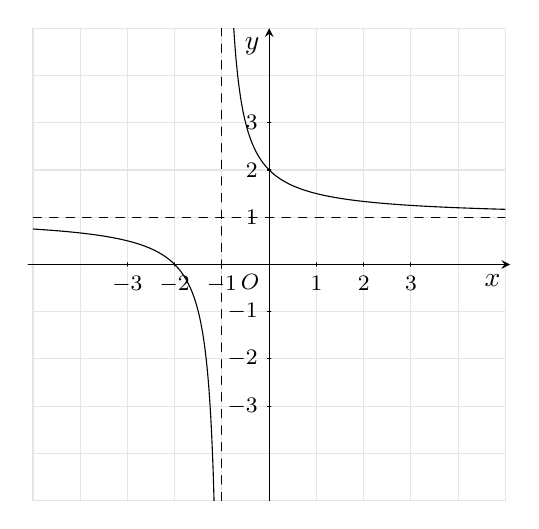
\begin{tikzpicture}[line join=round,line cap=round,>=stealth,scale=0.6]
		\draw[gray!20](-5,-5)  grid (5,5);
		\draw[->] (-5.1,0)--(5.1,0) node[below left] {$x$}; 
		\draw[->] (0,-5)--(0,5) node[below  left] {$y$};
		\draw (0,0)  node [below left] {\footnotesize $O$};
		\foreach \x in  {-3,-2,-1,1,2,3}
		\draw[thin] (\x,1pt)--(\x,-1pt) node [below]  {\footnotesize $\x$};
		\foreach \y  in {-3,-2,-1,1,2,3}
		\draw[thin] (1pt,\y)--(-1pt,\y) node [left] {\footnotesize $\y$}; 
		\begin{scope}
			\clip (-5,-5)  rectangle (5,5);
			 \draw[samples=100,domain=-5:-1.1,smooth,variable=\x]
				plot  (\x,{((\x)+2)/((\x)+1)});
			\draw[samples=100,domain=-0.9:5,smooth,variable=\x] 
				 plot (\x,{((\x)+2)/((\x)+1)});
			\draw[samples=100,domain=-5:5,smooth,dashed,variable=\x] 
				plot (\x,{1/1}); 
			\draw[dashed]  (-1/1,-5)--(-1/1,5);
		\end{scope}
	\end{tikzpicture}
		 }}
	 \loigiai{
		Vì $\lim\limits_{x \to -\infty  } f(x)= 1$; $\lim\limits_{x \to +\infty } f(x)=1$. Nên đồ thị hàm số có tiệm cận ngang là $y=1$.
	} 
\end{ex}

% nguồn: Phan1_Lop_12_Dai_so_Chuong_1
\begin{ex}%[2D1N3-1]%[ma:9d499163]
	Cho hàm số $y=f(x)$ có đồ thị như  hình vẽ. Gọi $m$ và $M$ lần lượt là giá trị nhỏ nhất và giá trị lớn nhất của hàm số $f(x)$ trên đoạn $[-1; 1]$.
	\begin{center}
		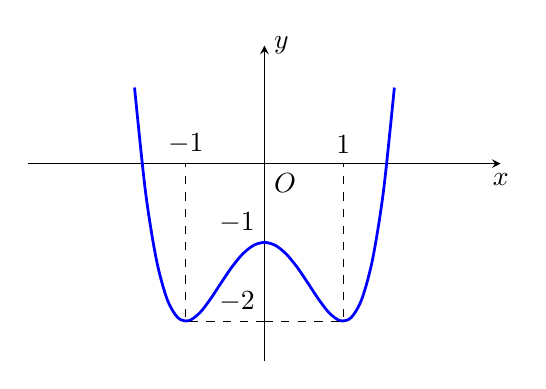
\begin{tikzpicture}[>=stealth]
			\draw[->] (-3,0)  --(0,0) node[below
				right]{$O$} --  (3,0)
				 node[below]{$x$};
			\draw[->](0,-2.5)--(0,1.5) 
				node[right]{$y$}; 
			 \draw[smooth,blue,line width=1]
				plot[domain=-1.65:1.65] 
				(\x,{(\x)^(4)-2*(\x)^(2)-1}); 
			\draw[dashed]  (0,-2)
				node[left]{}  -- (1,-2) --
				(1,0)  node[above]{$1$};
			\draw[dashed]  (0,-2)
				node[above left]{$-2$} -- (-1,-2) -- 
				(-1,0) node[above]{$-1$}; 
			\draw (0,-1) node[above  left] {$-1$};
		\end{tikzpicture}
	\end{center}
	Khẳng định  nào sau đây là đúng?
	 \choice
		{$m+M=2$} 
		 {$m+M=-2$}
		{$m+M=0$} 
		 {\True $m+M=-3$}
	 \loigiai{
		Dựa vào đồ thị, ta  thấy trên đoạn $[-1; 1]$, hàm số đạt:\\
		Giá trị lớn  nhất $M=-1$ tại $x=0$.\\
		Giá trị nhỏ nhất $m=-2$ tại $x= \pm1$.\\ 
	Suy ra  $m+M=-3$.}
\end{ex}

% nguồn: Phan1_Lop_12_Dai_so_Chuong_1
\begin{ex}%[2D1N3-1]%[ma:ef733eb4]
	 Cho $ac\neq 0$, $ad-bc\neq 0$. Đồ thị hàm số $y=\dfrac{ax+b}{cx+d}$ có đường tiệm cận đứng là
	 \choice
		{$x=\dfrac{a}{c}$} 
		{\True  $x=\dfrac{-d}{c}$}
		 {$y=\dfrac{a}{c}$}
		 {$y=\dfrac{-d}{c}$}
	 \loigiai{
		Đồ thị hàm số có tiệm  cận đứng là $x=-\dfrac{d}{c}$.
	 }
\end{ex}

% nguồn: Phan1_Lop_12_Dai_so_Chuong_1
\begin{ex}%[2D1N3-1]%[ma:9c43b999]
	Gọi $M$ và  $m$ lần lượt là giá trị lớn nhất và giá trị nhỏ nhất của hàm số $y=\sqrt{1-x}+\sqrt{1+x}$. Giá trị của $M-2 m^2$ bằng
	 \choice
		 {\True $-2$}
		{$2$} 
		 {$0$}
		{$-1$} 
	\loigiai{Điều kiện xác định $\heva{&1-x \geq 0 \\& x+1 \geq  0} \Leftrightarrow-1 \leq x \leq 1$.\\
		Xét hàm số $f(x)=\sqrt{1-x}+\sqrt{1+x}$ trên $[-1; 1]$, có $f'(x)=-\dfrac{1}{2  \sqrt{1-x}}+\dfrac{1}{2 \sqrt{1+x}}$;\\
		Phương trình $f'(x)=0 \Leftrightarrow  \heva{&-1<x<1 \\& \sqrt{1-x}=\sqrt{1-x}} \Leftrightarrow x=0 $. \\
		Tính $f(-1)=f(1)=\sqrt{2};  f(0)=2$.\\
		Vậy  $\heva{&m=\min\limits _{[-1; 1]} f(x)=\sqrt{2} \\& M=\max \limits_{[-1; 1]} f(x)=2}\rightarrow M-2 m^2=2-2\cdot2=-2$.
	} 
\end{ex}

% nguồn: Phan1_Lop_12_Dai_so_Chuong_1
\begin{ex}%[2D1N3-1]%[ma:30d94805]
	Cho $acd\neq 0$. Đồ thị hàm số $y=ax+b+\dfrac{c}{dx+e}$ ($a$, $b$,  $c$, $d$, $e\in\mathbb{R})$ có đường tiệm cận xiên là
	\choice 
		{\True  $y=ax+b$}
		{$y=dx+c$} 
		{$y=bx+a$} 
		 {$y=ex+d$}
	 \loigiai{
		Vì $\lim\limits_{x \to \pm \infty} [y-(ax+b)]=\lim\limits_{x \to \pm \infty} \dfrac{c}{dx + e}=0$ nên đồ  thị hàm số có tiệm cận xiên là $y = ax + b$.
	} 
\end{ex}

% nguồn: Phan1_Lop_12_Dai_so_Chuong_1
\begin{ex}%[2D1N3-1]%[ma:3f5d9bc4]
	\immini{Cho hàm số $y=f(x)$ liên tục trên $\mathbb{R}$ và có đồ thị như \textit{Hình 1}. Giá trị nhỏ nhất của hàm số trên  đoạn $[-2; 2]$ là
	\choice 
		{$-2$} 
		{$-1$} 
		{$1$} 
		{\True  $-3$}
		 }{\resizebox{!}{5cm}{
		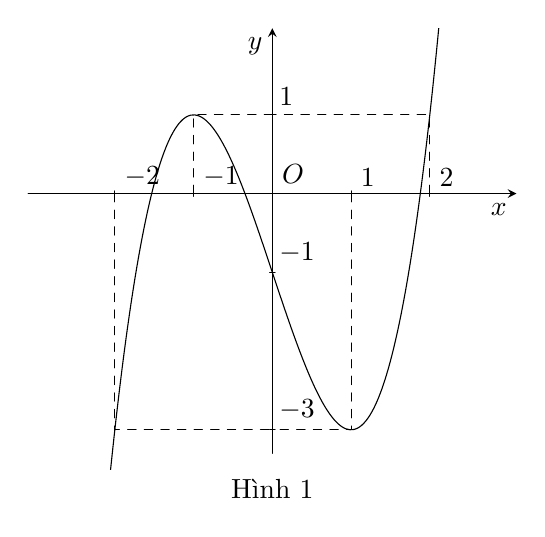
\begin{tikzpicture}[line join=round,line cap=round,>=stealth]
			 \draw[->] (-3.1,0)--(3.1,0) node[below left] {$x$};
			\draw[->] (0,-3.3)--(0,2.1) node[below  left] {$y$};
			 \draw[dashed] (-2,0)--(-2,-3)--(0,-3)
				 (1,0)--(1,-3)--(0,-3)
				 (2,0)--(2,1)--(0,1)
				(-1,0)--(-1,1)--(0,1); 
			\draw (0,0) node [above right] {$O$}; 
			\foreach \x  in {-2,-1,1,2}
			\draw[thin] (\x,1pt)--(\x,-1pt) node [above right] {$\x$}; 
			\foreach \y in  {-3,-1,1}
			\draw[thin] (1pt,\y)--(-1pt,\y) node [above right]  {$\y$};
			\begin{scope}
				\clip (-2.5,-3.5) rectangle (2.5,2.1); 
				\draw[samples=100,domain=-2.5:2.5,smooth,variable=\x] plot  (\x,{((\x)^3)-0*((\x)^2)-3*(\x)-1});
			\end{scope}
			\draw (0,-4) node [above] {Hình 1}; 
		\end{tikzpicture}
		} 
		 }
	\loigiai{ 
		Từ đồ thị hàm số ta suy ra  giá trị nhỏ nhất của hàm số trên đoan $[-2; 2]$ là $-3$.
	 }
\end{ex}

% nguồn: Phan1_Lop_12_Dai_so_Chuong_1
\begin{ex}%[2D1N3-1]%[ma:6f41dea5]
	 \immini{
	Cho hàm số $y=f(x)$ có  đồ thị như hình vẽ bên.
	Giá trị lớn  nhất của hàm số trên đoạn $[-3;4]$ bằng
	\choice 
		{$f(2)$} 
		{\True $f(-3)$} 
		{$f(4)$} 
		 {$f(0)$}}
		{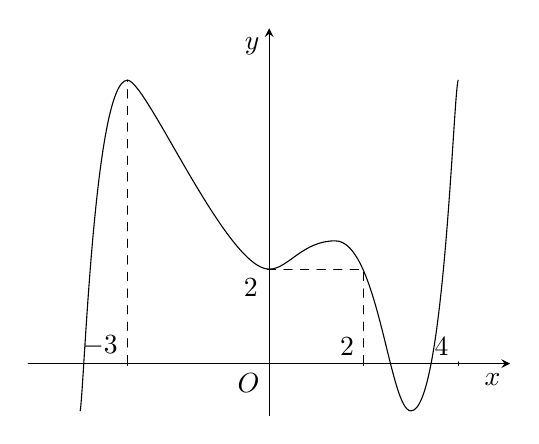
\begin{tikzpicture}[scale=0.6,line join=round,line cap=round,>=stealth]
		\tikzset{ethicknode/.style={scale=0.7}} 
		\draw[->] (-5.1,0)--(5.1,0) node[below left] {$x$}; 
		\draw[->]  (0,-1.1)--(0,7.1) node[below left] {$y$};
		\draw (0,0) node [below left] {$O$}; 
		 \foreach \x/\nx in {-3/-3,2/2,4/4}
		\draw[thin]  (\x,1pt)--(\x,-1pt) node [above left] {$\nx$};
		\foreach \y/\ny in  {2/2}
		\draw[thin] (1pt,\y)--(-1pt,\y) node [below left]  {$\ny$};
		\draw  (-4,-1)
			 ..controls+(80:0.5) and +(180:0.7)..(-3,6)
			..controls+(0:0.4)  and +(180:0.9)..(0,2)
			..controls+(0:0.4)  and +(180:0.7)..(1.4,2.6)
			..controls+(0:0.9) and  +(180:0.45)..(3,-1)
			..controls+(0:0.7) and +(-110:0.3)..(4,6); 
		\draw[dashed,thin] (-3,0)--(-3,6) 
			(2,0)--(2,2)--(0,2); 
	\end{tikzpicture}
		 }
	\loigiai{ 
		Quan sát đồ thị, ta thấy điểm $x=-3$ hàm số đạt giá  trị cao nhất trên đoạn $[-3;4]$.\\
		Vậy $\max\limits_{[-3;4]}f(x)=f(-3)$. 
	 }
\end{ex}

% nguồn: Phan1_Lop_12_Dai_so_Chuong_1
\begin{ex}%[2D1N3-1]%[ma:c67cfe5e]
	Giá trị  lớn nhất của hàm số $y=\dfrac{x+1}{x-3}$ trên đoạn $[0;2]$ bằng
	 \choice
		{$3$} 
		{$-3$} 
		{$\dfrac{1}{3}$} 
		 {\True$-\dfrac{1}{3}$}
	\loigiai{ 
		Ta có $y'=\dfrac{-4}{(x-3)^2}<0$ $\forall x\in[0;2]$, do đó  giá trị lớn nhất của hàm số $y=\dfrac{x+1}{x-3}$ trên đoạn $[0;2]$ bằng
	$y(0)=-\dfrac{1}{3}$.} 
\end{ex}

% nguồn: Phan1_Lop_12_Dai_so_Chuong_1
\begin{ex}%[2D1N3-1]%[ma:79ec24ff]
	Giá trị  nhỏ nhất của hàm số $f(x)=\dfrac{x^2+3}{x-1}$ trên đoạn $[2; 4]$ là
	 \choice
		 {$7$}
		{\True $6$} 
		{$\dfrac{19}{3}$} 
		{$\dfrac{13}{3}$} 
	\loigiai{ 
		Xét  hàm số $f(x)=\dfrac{x^2+3}{x-1}$ trên $[2; 4]$, có $f'(x)=\dfrac{x^2-2 x-3}{(x-1)^2}$\\
		 Phương trình $f'(x)=0 \Leftrightarrow $ $\heva{&2 \leq x \leq 4 \\ & x^2-2x-3=0 }$
		$ \Leftrightarrow  x=3.$\\
		 Tính $f(2)=7; f(3)=6; f(4)=\dfrac{19}{3} $.\\
		Vậy $\min\limits _{[2; 4]}  f(x)=f(3)=6 $.
	} 
\end{ex}

% nguồn: Phan1_Lop_12_Dai_so_Chuong_1
\begin{ex}%[2D1N3-1]%[ma:be38ac7f]
	Đường thẳng $x = a$ được gọi là  một đường tiệm cận đứng (hay tiệm cận đứng) của đồ thị hàm số $ y = f (x)$ nếu điều kiện sau thoả mãn
	\choice 
		 {$\lim\limits_{x\to +\infty }f(x)=a$}
		 {\True $\lim\limits_{x\to a^-}f(x)=+\infty $}
		{$\lim\limits_{x\to -\infty }f(x)=a$} 
		{$\lim\limits_{x\to  a^-}f(x)=a $}
	\loigiai{Đường thẳng $x = a$ được gọi là một đường tiệm cận đứng của đồ thị hàm số $y = f (x)$ nếu ít nhất một trong các điều kiện sau thoả mãn $$\lim\limits_{x\to a^+} f(x) = +\infty, \lim\limits_{x\to a^+} f(x) = -\infty, \lim\limits_{x \to a^-}f(x) = -\infty , \lim\limits_{x\to a^-} f(x)  = +\infty .$$
	 }
\end{ex}

% nguồn: Phan1_Lop_12_Dai_so_Chuong_1
\begin{ex}%[2D1N3-1]%[ma:ca46013d]
	 \immini{
	 Cho hàm số $f(x)$ liên tục trên $\mathbb{R}$ và có đồ thị như hình vẽ. Giá trị lớn nhất của $f(x)$ trên đoạn $[1;2]$ bằng
	\choice 
		{$-1$} 
		{$0$} 
		{\True  $1$}
		 {$2$}
		} 
		 {
		\begin{tikzpicture}[scale=1,font=\footnotesize,line join=round,line cap=round,>=stealth]
			\draw[->]  (-3.1,0)--(3.1,0) node[below left] {$x$};
			\draw[->] (0,-2.1)--(0,3.1) node[below left]  {$y$};
			\draw (0,0) node [below  left] {$O$};
			\foreach \x/\gx in  {-1/-1,2/2}
			\draw (\x,1pt)--(\x,-1pt) node [below]  {$\gx$};
			\foreach  \y/\gy in {-1/-1,1/1}
			\foreach \x/\gx in  {-2/-2,1/1}
			\draw (\x,1pt)--(\x,-1pt) node [above]  {$\gx$};
			\foreach  \y/\gy in {-1/-1,1/1}
			\draw (1pt,\y)--(-1pt,\y) node [above left]  {$\gy$};
			\draw[dashed](1,0)--(1,-1)--(0,-1); 
			\draw[dashed](-1,0)--(-1,1)--(0,1); 
			 \draw[dashed](2,0)--(2,1)--(0,1);
			\draw[dashed](-2,0)--(-2,-1)--(0,-1); 
			\begin{scope}
				 \clip (-3,-2) rectangle (3,3);
				\draw[samples=100,domain=-3:3,smooth,variable=\x] plot  (\x,{0.5*((\x)^3)+0*((\x)^2)+-1.5*(\x)+0});
			\end{scope}
		\end{tikzpicture}
		} 
	\loigiai{ 
		Từ  bảng biến thiên suy ra $\max\limits_{[1; 2]}f(x)=1$ tại $x=2$.
	 }
\end{ex}

% nguồn: Phan1_Lop_12_Dai_so_Chuong_1
\begin{ex}%[2D1N3-1]%[ma:958be4d6]
	\immini{Một trong bốn đường thắng dưới đây là đường tiệm cận dứng của đồ thị hàm số ơ hinh bên. Hói đường tiệm cận đứng của đổ thị hàm số  đó là đường nào?
	\choice 
		{\True  $x=-1$}
		 {$x=-2$}
		{$y=1$} 
		 {$y=2$}}
		{\resizebox{!}{5cm}{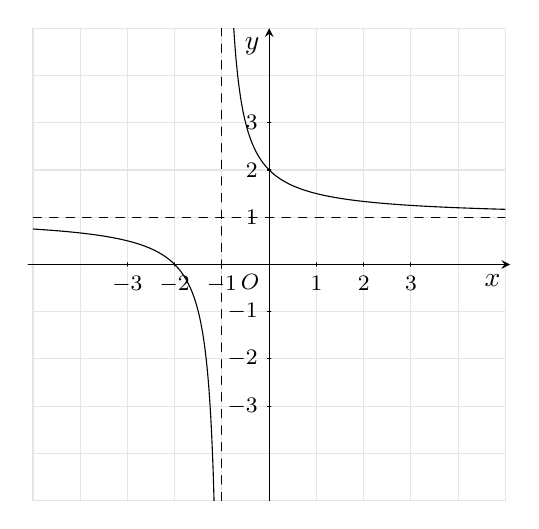
\begin{tikzpicture}[line join=round,line cap=round,>=stealth,scale=0.6]
		 \tikzset{ethicknode/.style={scale=0.9}}
		\draw[gray!20](-5,-5) grid (5,5); 
		\draw[->] (-5.1,0)--(5.1,0) node[below  left] {$x$};
		\draw[->] (0,-5)--(0,5) node[below left]  {$y$};
		\draw (0,0) node [below left] {\footnotesize $O$}; 
		\foreach \x in {-3,-2,-1,1,2,3} 
		\draw[thin] (\x,1pt)--(\x,-1pt) node [below] {\footnotesize  $\x$};
		\foreach \y in {-3,-2,-1,1,2,3} 
		 \draw[thin] (1pt,\y)--(-1pt,\y) node [left] {\footnotesize $\y$};
		\begin{scope}
			\clip (-5,-5) rectangle  (5,5);
			 \draw[samples=100,domain=-5:-1.1,smooth,variable=\x]
				 plot (\x,{((\x)+2)/((\x)+1)});
			 \draw[samples=100,domain=-0.9:5,smooth,variable=\x]
				 plot (\x,{((\x)+2)/((\x)+1)});
			\draw[samples=100,domain=-5:5,smooth,dashed,variable=\x] 
				 plot (\x,{1/1});
			 \draw[dashed] (-1/1,-5)--(-1/1,5);
		\end{scope}
	\end{tikzpicture}
		 }}
	 \loigiai{
		Vì $\lim\limits_{x \to (-1)^-} f(x)=-\infty$; $\lim\limits_{x \to (-1)^+} f(x)=+\infty$ Nên đồ thị hàm số có tiệm cận đứng là  $x=-1$.
	 }
\end{ex}

% nguồn: Phan1_Lop_12_Dai_so_Chuong_1
\begin{ex}%[2D1N3-1]%[ma:6e8be730]
	Cho $ac \neq 0$,$ad-bc\neq 0$. Đồ thị hàm số $y=\dfrac{ax+b}{cx+d}$ có đường  tiệm cận ngang là
	\choice 
		 {$x=\dfrac{a}{c}$}
		{$x=\dfrac{-d}{c}$} 
		{\True  $y=\dfrac{a}{c}$}
		 {$\mathrm{y}=\dfrac{-d}{c}$}
	\loigiai{ 
		Đồ  thị hàm số có tiệm cận ngang là $y=\dfrac{a}{c}$.
	} 
\end{ex}

% nguồn: Phan1_Lop_12_Dai_so_Chuong_1
\begin{ex}%[2D1N3-1]%[ma:876cbdc1]
	Giá trị nhỏ nhất $m$  của hàm số $y=x^{3}-8 x^{2}+16 x-9$ trên đoạn $[1; 3]$ bằng
	 \choice
		{$m=0$} 
		{$m=-9$} 
		 {$m=\dfrac{13}{27}$}
		{\True $m=-6$} 
	 \loigiai{
		Ta  có\\
		$y'=3x^2 -16x  +16$.\\
		$y'=0 \Leftrightarrow \hoac{ 
		&x=4 \notin  [1; 3]\\
		 &x=\dfrac{4}{3} \in [1; 3].}$\\
		$y(1)=0$;  $y\left(\dfrac{4}{3}\right)=\dfrac{13}{27}$; $y(3)=-6$.\\
		Vậy  $\min_{[1; 3]} y=-6$ khi $x=3$.
	} 
\end{ex}

% nguồn: Phan1_Lop_12_Dai_so_Chuong_1
\begin{ex}%[2D1N3-1]%[ma:87303cde]
	 \immini{
	Cho hàm số $f(x)=ax^3+bx^2+cx+d$ có đồ thị  như hình vẽ bên
	Giá trị lớn nhất của hàm số đã  cho trên đoạn $[-3;3]$ bằng
	 \choice
		{\True $f(-3)$} 
		{$f(-1)$} 
		{$f(2)$} 
		 {$f(3)$}
		}{\begin{tikzpicture}[scale=0.6,line join=round,line cap=round,>=stealth]
		 \tikzset{ethicknode/.style={scale=0.9}}
		 \draw[->] (-4.1,0)--(4.1,0) node[below left] {$x$};
		\draw[->] (0,-1.1)--(0,7.1) node[below left] {$y$}; 
		\draw (0,0) node [below right] {$O$}; 
		\foreach \x/\nx in  {-3/-3,-1/-1,2/2,3/3}
		\draw[thin] (\x,1pt)--(\x,-1pt) node  [below] {$\nx$};
		\draw (-3.2,6) 
			 ..controls+(-80:0.5) and +(180:0.9)..(-1,1.5)
			..controls+(0:0.8) and +(180:0.7)..(2,4) 
			..controls+(0:0.8)  and +(110:0.4)..(3.5,1.5);
		\draw[dashed,thin] (-3,0)--(-3,5.25) 
			 (2,0)--(2,4)
			(-1,0)--(-1,1.5) 
			 (3,0)--(3,2.8);
	\end{tikzpicture}
		 }
	 \loigiai{
		Dựa vào đồ thị, ta thấy hàm số  đạt giá trị lớn nhất tại đầu trái đoạn $[-3; 3]$ là $x=-3$.\\
		Vậy  $\max\limits_{[-3;3]}f(x)=f(-3)$.
	 }
\end{ex}

% nguồn: Phan1_Lop_12_Dai_so_Chuong_1
\begin{ex}%[2D1N3-1]%[ma:3e255c90]
	Cho hàm số $y=f(x)$ liên tục trên $[-3; 2]$ và có bảng biến thiên như hình dưới đây. Gọi $M$ và $m$ lần lượt là giá trị lớn nhất và giá  trị nhỏ nhất của hàm số $y=f(x)$ trên $[-1; 2]$.
	\begin{center}
		
\begin{tikzpicture}
			 \tkzTabInit[nocadre=false,lgt=0.7,espcl=2.1,deltacl=0.5]
				{$x$ /0.7,$y'$ /0.7,$y$ /2} 
				 {$-3$,$-1$,$0$,$1$,$2$}
			\tkzTabLine{,+,$0$,-,$0$,+,$0$,-,} 
			\tkzTabVar{-/$2$,+/$3$,-/$0$,+/$2$,-/$1$} 
		\end{tikzpicture}
	\end{center}
	Giá trị  của $5M-2m$ bằng bao nhiêu?
	 \choice
		{\True  $15$}
		 {$3$}
		{$17$} 
		 {$-15$}
	 \loigiai{
		 Ta có $M=\max \limits_{[-1; 2]} f(x)=f(-1)=3$ và $m=\min\limits _{[-1; 2]} f(x)=f(0)=0$.\\
		 Vậy $5M-2m=15$.
	 }
\end{ex}

% nguồn: Phan1_Lop_12_Dai_so_Chuong_1
\begin{ex}%[2D1N3-1]%[ma:1c4696c7]
	Tìm giá trị nhỏ nhất  của hàm số $y=x^3-24x+1$ trên đoạn $[2;19]$.
	 \choice
		 {\True $1-32\sqrt{2}$}
		{$-39$} 
		 {$1+32\sqrt{2}$}
		{$-44$} 
	\loigiai{ 
		Hàm số liên tục trên  đoạn $[2;19]$.\\
		Ta có  $y'=3x^2-24$.\\
		Xét $y'=3x^2-24=0 \Leftrightarrow x^2=8 \Leftrightarrow x=\pm  2\sqrt{2}$\\
		$y(2)=2^3-24 \cdot  2+1=-39$.\\
		$y(19)=19^3-24 \cdot 19+1=6404$.\\ 
		$y\left( 2\sqrt{2}\right) =\left( 2\sqrt{2}\right) ^3-24 \cdot  2\sqrt{2}+1=-32\sqrt{2}+1$.\\
		Giá trị  nhỏ nhất của hàm số trên đoạn $[2;19]$ là $y\left( 2\sqrt{2}\right)=-32\sqrt{2}+1$.
	} 
\end{ex}

% nguồn: Phan1_Lop_12_Dai_so_Chuong_1
\begin{ex}%[2D1N3-1]%[ma:9c807092]
	Tìm giá trị nhỏ  nhất của hàm số $y=\dfrac{x+3}{x-1}$ trên đoạn $[-1;0]$.
	\choice 
		{\True $\displaystyle\min\limits_{[-1;0]}y=-3$} 
		 {$\displaystyle\min\limits_{[-1;0]}y=-2$}
		 {$\displaystyle\min\limits_{[-1;0]}y=-4$}
		 {$\displaystyle\min\limits_{[-1;0]}y=3$}
	\loigiai{Hàm số $y=\dfrac{x+3}{x-1}$ xác định  trên đoạn $[-1;0]$.\\
		Ta có $y'=\dfrac{-4}{(x-1)^2}<0$  $\forall x\in [-1;0]$.\\
	Vậy  $\min\limits_{[-1;0]} y=y(0)=-3$.}
\end{ex}

% nguồn: Phan1_Lop_12_Dai_so_Chuong_1
\begin{ex}%[2D1N3-1]%[ma:4aa66e72]
	Cho hàm số $y=f(x)$ liên tục trên $\mathbb{R}$  và có đồ thị như \textit{Hình 1}. Giá trị lớn nhất của hàm số trên đoạn $[-2; 2]$ là
	\choice 
		{$2$} 
		 {$-1$}
		 {\True $1$}
		 {$-3$}
	\loigiai{ 
		Từ đồ  thị hàm số ta suy ra giá trị lớn nhất của hàm số trên đoạn $[-2; 2]$ là $1$.
	 }
\end{ex}

% nguồn: Phan1_Lop_12_Dai_so_Chuong_1
\begin{ex}%[2D1N3-1]%[ma:249d8128]
	Gọi $M, m$ lần lượt là giá trị lớn nhất, giá trị nhỏ nhất của hàm số  $f(x)=\dfrac{3 x-1}{x-3}$ trên đoạn $[0; 2]$.
	Giá trị  của $3 M+m$ bằng
	\choice 
		 {$0$}
		 {$-4$}
		{\True  $-2$}
		{$1$} 
	\loigiai{Xét hàm số $f(x)=\dfrac{3  x-1}{x-3}$ trên $[0; 2]$ có $f'(x)=-\dfrac{8}{(x-3)^2}<0$.\\
		Suy ra $f(x)$  là hàm số nghịch biến trên $(0; 2) \Rightarrow \heva{& \min\limits _{[0; 2]} f(x)=f(2)=-5 \\& \max\limits _{[0; 2]} f(x)=f(0)=\dfrac{1}{3}.}$\\
		Vậy $M=\dfrac{1}{3} \Rightarrow  3 M=3; m=-5 \Rightarrow 3 M+m=-2$.
	 }
\end{ex}

% nguồn: Phan1_Lop_12_Dai_so_Chuong_1
\begin{ex}%[2D1N3-1]%[ma:dc0c3cfd]
	\immini 
	{Cho đồ thị hàm số $y =  f(x)$ có đồ thị như hình vẽ. Khẳng định nào là đúng?
	\choice 
		{Đồ thị hàm số chỉ có 2 đường tiệm cận đứng là các đường  thẳng $x=-1$ và $x=1$}
		{\True Đồ thị  hàm số có 3 đường tiệm cận}
		{Đồ thị hàm số  có 4 đường tiệm cận}
		{Đồ thị hàm số có  2 đường tiệm cận đứng và 1 đường tiệm cận xiên}
		} 
		{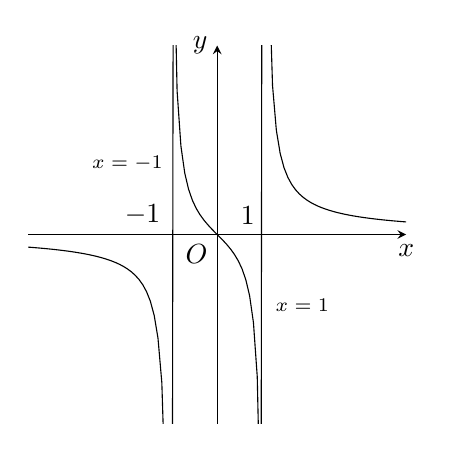
\begin{tikzpicture}[>=stealth,scale=0.6]
		\draw[->]  (-4,0) --(4,0);
		 \draw[->](0,-4)--(0,4);
		\draw (0,0)  node[below left]{$O$};
		 \draw (4,0) node[below]{$x$};
		\draw (0,4) node[left]{$y$}; 
		 \draw (1,0) node[above left]{$1$};
		\draw (-1,0)  node[above left]{$-1$};
		\clip (-4,-4)  rectangle (4,4);
		\draw[samples=100]  plot[domain=-4:4]
			(\x,{(\x)/((\x)^(2)-1)}); 
		\draw (-1.9,1.5) node {\scriptsize $x=-1$}; 
		\draw  (1.8,-1.5) node {\scriptsize $x=1$};
	\end{tikzpicture}
		} 
	\loigiai{Đồ thị hàm số có 2 đường tiệm cận đứng $x=-1$ và $x=1$ và một đường tiệm cận ngang $y=0$, hàm số không có  đường tiệm cận xiên.}
\end{ex}

% nguồn: Phan1_Lop_12_Dai_so_Chuong_1
\begin{ex}%[2D1N3-1]%[ma:ecdd7b5a]
	Cho hàm số  $y=f(x)$ thoả mãn $\lim\limits_{x \to - \infty } [f(x)-5x+7]=0$. Đường tiệm cận xiên của đồ thị hàm số $y=f(x)$ là
	 \choice
		 {\True $y=5x-7$}
		 {$y=5x+7$}
		 {$y=-5x-7$}
		 {$y=5x+7$}
	\loigiai{ 
		Vì $\lim\limits_{x \to - \infty} [f(x)-5x+7]=0\Leftrightarrow \lim\limits_{x \to -\infty} [f(x)-(5x-7)]=0$ nên  đồ thị hàm số có tiệm cận xiên là $y=5x-7$.
	} 
\end{ex}

% nguồn: Phan1_Lop_12_Dai_so_Chuong_1
\begin{ex}%[2D1N3-1]%[ma:ede13f5a]
	Đường thẳng $y = ax + b, a \neq 0$, được  gọi là đường tiệm cận xiên (hay tiệm cận xiên) của đồ thị hàm số $y = f(x)$ nếu
	\choice 
		{\True $\lim\limits_{x\to -\infty }(f(x)-ax-b)=0$ hoặc $\lim\limits_{x\to +\infty }(f(x)-ax-b)=0$} 
		 {$\lim\limits_{x\to -\infty }(f(x)-ax+b)=0$ hoặc $\lim\limits_{x\to +\infty }(f(x)-ax+b)=0$}
		{$\lim\limits_{x\to 0  }[f(x)-(ax+b)]=+\infty $ hoặc $\lim\limits_{x\to 0 }[f(x)-(ax+b)]=-\infty $}
		{$\lim\limits_{x\to -\infty }(f(x)-ax+b)=a$  hoặc $\lim\limits_{x\to +\infty }(f(x)-ax+b)=a$}
	\loigiai{Đường thẳng $y = ax + b, a \neq 0$, được gọi là đường tiệm cận xiên  (hay tiệm cận xiên) của đồ thị hàm số $y = f(x)$ nếu\\ $\lim\limits_{x\to -\infty }[f(x)-(ax+b)] = \lim\limits_{x\to -\infty} (f(x)-ax-b) = 0$ hoặc\\ $\lim\limits_{x\to +\infty }[f(x)-(ax+b)] = \lim\limits_{x \to +\infty }(f(x)-ax-b) = 0$.
	 }
\end{ex}

% nguồn: Phan1_Lop_12_Dai_so_Chuong_1
\begin{ex}%[2D1N3-1]%[ma:0456acba]
	Cho hàm số phù hợp với bảng biến thiên sau 
	\begin{center}
		
\begin{tikzpicture}
			\tkzTabInit[nocadre,lgt=1.5,espcl=2.5] 
				{$x$ /1,$y'$ /1,$y$  /2}
				 {$-\infty$,$2$,$+\infty$}
			\tkzTabLine{,+,0,-} 
			\tkzTabVar{-/$-1$,+/ $1$ /,-/$1$} 
		\end{tikzpicture}
	\end{center}
	Phát biểu nào sau đây là  đúng?
	\choice 
		{\True Đồ thị hàm số có hai đường tiệm  cận ngang là $y=-1$, $y=1$}
		{Đồ thị hàm  số có hai đường tiệm cận ngang là $x=-1$, $x=1$}
		{Đồ thị hàm  số không có đường tiệm cận ngang}
		{Đồ thị hàm  số có đường tiệm cận đứng}
	\loigiai{ 
		Vì $\lim\limits_{x \to - \infty } f(x)=-1$; $\lim\limits_{x \to +\infty} f(x)=1$ nên đồ thị hàm  số có haitiệm cận ngang là $y=-1$ và $y=1$.
	 }
\end{ex}

% nguồn: Phan1_Lop_12_Dai_so_Chuong_1
\begin{ex}%[2D1N3-1]%[ma:9a8cdfa9]
	\immini{ 
	Cho hàm số $f(x)$ liên tục trên đoạn $[-2;2]$ có đồ  thị như hình vẽ bên
	Giá trị nhỏ nhất của  hàm số trên đoạn $[-2;2]$ là
	 \choice
		 {$1$}
		{\True $-1$} 
		{$-2$} 
		{$3$} 
		}{\begin{tikzpicture}[line join=round,line cap=round,>=stealth]
		 \tikzset{ethicknode/.style={scale=0.9}}
		\draw[->]  (-3.1,0)--(3.1,0) node[below left] {$x$};
		\draw[->] (0,-2.1)--(0,4.1) node[below left]  {$y$};
		\draw (0,0) node [below left] {$O$}; 
		\foreach \x/\nx  in {-2/-2,-1/-1,1/1,2/2}
		\draw[thin] (\x,1pt)--(\x,-1pt) node [above  left] {$\nx$};
		\foreach \y/\ny in {-1/-1,1/1,3/3} 
		\draw[thin] (1pt,\y)--(-1pt,\y) node  [below left] {$\ny$};
		\draw[dashed,thin](-2,0)--(-2,-1)--(1,-1)--(1,0) 
			 (-1,0)--(-1,3)--(0,3)--(2,3)--(2,0);
		\begin{scope}
			\clip (-3,-2) rectangle (4,4); 
			\draw[samples=200,domain=-2:2,smooth,variable=\x]  plot (\x,{1*((\x)^3)-3*(\x)+1});
		\end{scope}
	\end{tikzpicture}
		} 
	\loigiai{ 
		Trên đoạn $[-2;2]$, quan sát đồ thị ta  thấy
		$f(x)\ge  -1$ và $f(x)=-1\Leftrightarrow\hoac{&x=-2\\&x=1.}$\\
		 Vậy $\min\limits_{[-2;2]}f(x)=-1$.
	 }
\end{ex}

% nguồn: Phan1_Lop_12_Dai_so_Chuong_1
\begin{ex}%[2D1H3-1]%[ma:84ab638b]
	Gọi $M$, $m$ lần lượt là giá trị lớn nhất, giá trị  nhỏ nhất của hàm số $y=\dfrac{1}{3}x^3-2x^2+3x+1$ trên đoạn $[0;4]$. Tính tổng $S=M+m$.
	\choice 
		 {$\dfrac{7}{3}$}
		 {$1$}
		{\True  $\dfrac{10}{3}$}
		{$4$} 
	\loigiai{ 
		Dễ  thấy hàm số liên tục trên $\mathbb{R}$.\\
		Ta có $y'=x^2-4x+3=0\Leftrightarrow\hoac{&x=1\\&x=3.}$\\ 
		Tính giá trị tại các điểm 
		 $\heva{
		 &y(0)=1\\
		&y(1)=\dfrac{7}{3}\\ 
		 &y(3)=1\\
		&y(4)=\dfrac{7}{3}. 
		}$\\ 
		Suy  ra
		$$\max\limits_{[0;4]}y=\dfrac{7}{3}\text{  và }\min\limits_{[0;4]}y=1\Rightarrow S=M+m=\dfrac{7}{3}+1=\dfrac{10}{3}.$$
	} 
\end{ex}

% nguồn: Phan1_Lop_12_Dai_so_Chuong_1
\begin{ex}%[2D1H3-1]%[ma:1673e727]
	Giá trị  lớn nhất của hàm số $y=\sqrt{-x^2+3x+4}$ là bao nhiêu?
	 \choice
		{\True $\dfrac{5}{2}$} 
		 {$\dfrac{2}{5}$}
		 {$\dfrac{3}{2}$}
		{$0$} 
	 \loigiai{
		Tập xác  định: $\mathscr D=\left[-1;4\right]$.\\ Ta có $y'=\dfrac{-2x+3}{2\sqrt{-x^2+3x+4}}. $\\
		Cho $y'=0\Leftrightarrow x=\dfrac{3}{2}$.\\ 
		Khi  đó $y\left(-1\right)=0;\, y(4)=0;\, y\left(\dfrac{3}{2} \right)=\dfrac{5}{2}$.\\ Vậy ${\mathop{\max}\limits_{\left[-1;4\right]}} y=\dfrac{5}{2}$.
	 }
\end{ex}

% nguồn: Phan1_Lop_12_Dai_so_Chuong_1
\begin{ex}%[2D1H3-1]%[ma:eda85393]
	Tìm giá trị lớn nhất $M$ của hàm số $y=\dfrac{3x-1}{x-3}$ trên đoạn $[0;2]$. 
	\choice 
		 {$M=-\dfrac{1}{3}$}
		{$M=5$} 
		 {$M=-5$}
		{\True  $M=\dfrac{1}{3}$}
	\loigiai{ 
		Hàm số $y=\dfrac{3x-1}{x-3}$  xác định và liên tục trên đoạn $[0;2]$.\\
		 Ta có $y'=-\dfrac{8}{(x-3)^2}<0, \forall x \neq 3$.\\
		Lại  có $y(0)=\dfrac{1}{3}$, $y(2)=-5$.\\
		Vậy  $M=\max\limits_{[1;3]}y=\dfrac{1}{3}$ tại $x=0$.
	 }
\end{ex}

% nguồn: Phan1_Lop_12_Dai_so_Chuong_1
\begin{ex}%[2D1H3-1]%[ma:d32100d4]
	Cho hàm số $f(x)$ xác định và liên tục trên $\mathbb{R}\setminus \{-1\}$  có bảng biến thiên như sau
	\begin{center}
		
\begin{tikzpicture}
			 \tkzTabInit[lgt=1.5,espcl=4,deltacl=.5]
				 {$x$/0.7,$f’(x)$/0.7,$f (x)$/2}
				 {$-\infty$,$-1$,$+\infty$}
			\tkzTabLine{,-,d,-,} 
			 \tkzTabVar{+/$5$,-D+/ $-\infty$/$+\infty$,-/$2$}
		\end{tikzpicture}
	\end{center}
	Khẳng định nào sau đây đúng? 
	 \choice
		{\True Đồ thị hàm số $f(x)$ có hai tiệm cận ngang  là các đường thẳng $y=2$, $y=5$ và có một tiệm cận đứng là đường thẳng $x=-1$}
		{Đồ  thị hàm số có bốn đường tiệm cận}
		{Đồ thị hàm số có  hai đường tiệm cận}
		{Đồ thị hàm số có một  đường tiệm cận}
	\loigiai{ 
		Dựa vào bảng biên thiên ta thấy hàm số $f(x)$ có 3 đường tiệm cận đó là hai tiệm cận ngang $y=2$, $y=5$  và có một tiệm cận đứng là đường thẳng $x=-1$.
	} 
\end{ex}

% nguồn: Phan1_Lop_12_Dai_so_Chuong_1
\begin{ex}%[2D1H3-1]%[ma:16270007]
	Trên đoạn  $\left[\dfrac{1}{3};\dfrac{3}{2}\right]$, hàm số $y=2x^3+\dfrac{1}{2x}$ đạt giá trị lớn nhất tại điểm nào sau đây?
	 \choice
		{$x=\dfrac{1}{2}$} 
		{\True  $x=\dfrac{3}{2}$}
		 {$x=\dfrac{1}{3}$}
		{$x=1$} 
	\loigiai{ 
		Tập xác định $\mathscr{D}=\mathbb{R}$.\\ 
		Ta  có $y'=6x^2-\dfrac{1}{2x^2}$.\\
		Suy ra 
		$y'=0\Leftrightarrow  12x^4=1\Leftrightarrow\hoac{
		 &x=\dfrac{1}{\sqrt[4]{12}}\in\left[\dfrac{1}{3};\dfrac{3}{2}\right]\\
		&x=\dfrac{-1}{\sqrt[4]{12}}\notin\left[\dfrac{1}{3};\dfrac{3}{2}\right]. 
		}$\\ 
		Ta có 
		$\heva{ 
		 &y\left(\dfrac{1}{3}\right)=\dfrac{85}{54}\\
		&y\left(\dfrac{1}{\sqrt[4]{12}}\right)=\dfrac{2}{\sqrt[4]{1728}}+\dfrac{\sqrt[4]{12}}{2}\\ 
		&y\left(\dfrac{3}{2}\right)=\dfrac{85}{12}. 
		 }$\\
		Vậy $\max\limits_{\left[\frac{1}{3};\frac{3}{2}\right]}y=y\left(\dfrac{3}{2}\right)$. 
	} 
\end{ex}

% nguồn: Phan1_Lop_12_Dai_so_Chuong_1
\begin{ex}%[2D1H3-1]%[ma:d465c9a2]
	Giá trị lớn nhất của hàm số $y=x^3+3x^2+10$ trên đoạn $[-5;-1]$ bằng 
	 \choice
		{$12$} 
		{$18$} 
		{$-40$} 
		{\True  $14$}
	\loigiai{ 
		Hàm số liên tục  trên đoạn $[-5;-1]$.\\
		Ta  có $y'=3x^2+6x=3x\cdot(x+2)=0\Leftrightarrow\hoac{&x=0\\&x=-2.}$\\
		 Trong đó $x=-2\in[-5;-1]$ là điểm cần xét.\\
		Ta  tính
		$\heva{ 
		&y(-5)=(-5)^3+3\cdot(-5)^2+10=-125+75+10=-40\\ 
		&y(-2)=(-2)^3+3\cdot(-2)^2+10=-8+12+10=14\\ 
		&y(-1)=(-1)^3+3\cdot(-1)^2+10=-1+3+10=12. 
		}$\\ 
		Vậy $\max\limits_{[-5;-1]}y=14$. 
	 }
\end{ex}

% nguồn: Phan1_Lop_12_Dai_so_Chuong_1
\begin{ex}%[2D1H3-1]%[ma:29718820]
	Cho hàm số $f(x)=-2 x^{4}+4 x^{2}+10$. Tìm giá trị  lớn nhất $M$ và giá trị nhỏ nhất $m$ của hàm số trên đoạn $[0; 2]$.
	\choice 
		 {$M=10; m=-6$}
		{\True$M=12;  m=-6$}
		 {$M=10; m=-8$}
		{$M=12;  m=-8$}
	 \loigiai{
		Ta có $f'(x)=-8x^3+8x$. \\ 
		$f'(x)=0 \Leftrightarrow \hoac{&x=0 \in  [0; 2]\\ &x=1\in [0; 2]\\&x=-1 \notin [0; 2].} $\\
		 Suy ra
		$\heva{&f(0)=10\\  &f(1)=12\\ &f(2)=-6}\Rightarrow \heva{&M=12\\&m=-6.}$
	 }
\end{ex}

% nguồn: Phan1_Lop_12_Dai_so_Chuong_1
\begin{ex}%[2D1H3-1]%[ma:19b30006]
	Cho hàm số $y=f(x)$ liên tục trên $[-3;2]$ và  có bảng biến thiên như hình dưới
	\begin{center}
		
\begin{tikzpicture}[>=stealth]
			 \tkzTabInit[nocadre=false,lgt=1,espcl=2,deltacl=0.5]
				 {$x$/.7,$f (x)$/2}
				 {$-3$,$0$,$1$,$2$}
			\tkzTabVar{-/$-4$,+/$2$,-/$0$,+/$1$} 
		\end{tikzpicture}
	\end{center}
	Gọi $M$, $m$ lần lượt là giá trị lớn nhất  và giá trị nhỏ nhất của hàm số $y=f(x)$ trên $[-3;2]$. Tính $M\cdot m$.
	 \choice
		{$6$} 
		{$7$} 
		 {$5$}
		{\True $-8$} 
	 \loigiai{
		Dựa  vào bảng biến thiên, ta xác định được
		$$M=2, m=-4\Rightarrow  M\cdot m=2\cdot(-4)=-8.$$
	} 
\end{ex}

% nguồn: Phan1_Lop_12_Dai_so_Chuong_1
\begin{ex}%[2D1H3-1]%[ma:00e0c271]
	Trên đoạn $[-4;-1]$, hàm  số $y=x+\dfrac{9}{x-1}$ đạt giá trị lớn nhất bằng
	 \choice
		{\True  $–5$}
		 {$\dfrac{-29}{5}$}
		 {$\dfrac{11}{2}$}
		{$4$} 
	\loigiai{ 
		Tập xác định $\mathscr{D}=\mathbb{R}\setminus\{1\}$.\\ 
		Ta có $y'=1-\dfrac{9}{(x-1)^2}$.\\ 
		Suy ra $y'=0\Leftrightarrow\left(x-1\right)^2=9\Leftrightarrow\hoac{ 
		&x=-2\in  [-4;-1]\\
		&x=4\notin [-4;-1]. 
		}$\\ 
		 Ta được
		$\heva{ 
		 &y(-4)=\dfrac{-29}{5}\\
		&y(-2)=-5\\ 
		 &y(-1)=\dfrac{-11}{2}.
		}$\\ 
		 Vậy $\max\limits_{[-4;-1]}y=y(-2)=-5$.
	 }
\end{ex}

% nguồn: Phan1_Lop_12_Dai_so_Chuong_1
\begin{ex}%[2D1H3-1]%[ma:039ebe92]
	Tìm giá trị nhỏ nhất $m$ của hàm số $y=x^3-3x+5$ trên  đoạn $[0;3]$.
	\choice 
		 {$m=7$}
		 {$m=5$}
		 {\True$m=3$}
		{$m=23$} 
	\loigiai{ 
		 Ta có $y'=3 x^2-3$.\\
		$y'=0 \Leftrightarrow 3 x^2-3=0 \Leftrightarrow\heva{&x=1  \in[0;3] \\&x=-1 \notin[0;3].}$\\
		 Ta có $y(0)=5$, $y(1)=3$, $y(3)=23$.\\
		Vậy $m=3$. 
	 }
\end{ex}

% nguồn: Phan1_Lop_12_Dai_so_Chuong_1
\begin{ex}%[2D1H3-1]%[ma:c63dc212]
	Gọi $m$, $M$ lần lượt là  giá trị nhỏ nhất, giá trị lớn nhất của hàm số $f(x)=4x+\sin ^2\pi x$ trên đoạn $\left[-1;2\right]$. Giá trị của $m+M$ bằng
	 \choice
		{$0$} 
		{\True $4$} 
		 {$-2$}
		{$-4$} 
	\loigiai{ 
		Ta có $f'(x)=4+2\pi \sin  \pi x \cdot \cos \pi x=4+\pi \sin 2\pi x$. \\
		Do $-1\le  \sin 2\pi x\le 1\Rightarrow f'(x) > 0, \, \forall x\in \left[-1;2\right]$.\\
		Suy ra $M=  f(2)$ và $m = f(-1)$.\\
		Vậy $m+M=f\left(-1\right)+f(2)=-4+\sin ^2\left(-\pi \right)+8+\sin  ^2\left(2\pi \right)=4$.
	} 
\end{ex}

% nguồn: Phan1_Lop_12_Dai_so_Chuong_1
\begin{ex}%[2D1H3-1]%[ma:f212334f]
	Gọi $m$, $M$ lần lượt là giá trị nhỏ nhất, giá trị lớn  nhất của hàm số $f(x)=2x+\cos \dfrac{\pi x}{2}$ trên đoạn $\left[-2; 2\right]$. Giá trị của $m+M$ bằng
	\choice 
		{$2$} 
		{\True $-2$} 
		 {$0$}
		 {$-4$}
	 \loigiai{
		Ta có $f'(x)=2-\dfrac{\pi}{2} \sin \dfrac{\pi x}{2} > 0,  \forall x\Rightarrow f(x)$ đồng biến trên $\left[-2; 2\right]$.\\
		 Khi đó $m+M=f\left(-2\right)+f(2)=-4-1+4-1=-2$.
	} 
\end{ex}

% nguồn: Phan1_Lop_12_Dai_so_Chuong_1
\begin{ex}%[2D1H3-1]%[ma:4e09f5b9]
	\immini{Một trong bốn đường thẳng dưới đây là đường tiệm cận xiên của đồ thị hàm số ở hình bên. Hỏi đường tiểm  cận xiên của đồ thị hàm số đó là đường nào?
	 \choice
		 {$y=x$}
		{\True  $y=x+1$}
		{$y=-x+1$} 
		 {$y=2x+1$}}
		{\resizebox{!}{5cm}{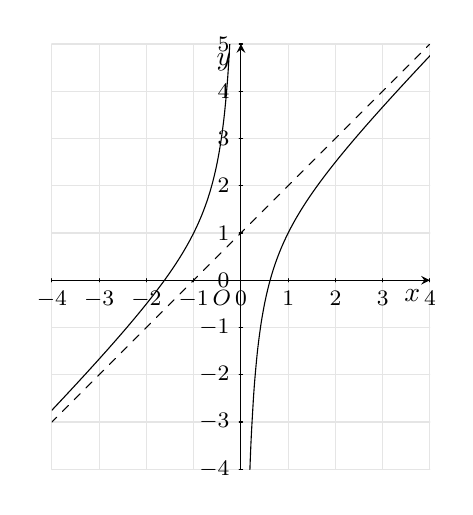
\begin{tikzpicture}[line join=round,line cap=round,>=stealth,scale=0.6]
		 \tikzset{ethicknode/.style={scale=0.9}}
		\draw[gray!20](-4,-4)  grid (4,5);
		\draw[->] (-4,0)--(4,0)  node[below left] {$x$};
		\draw[->] (0,-4)--(0,5) node[below left] {$y$}; 
		\draw (0,0) node [below left]  {\footnotesize $O$};
		\foreach \x  in {-4,-3,-2,-1,0,1,2,3,4}
		\draw[thin] (\x,1pt)--(\x,-1pt) node  [below] {\footnotesize $\x$};
		\foreach \y  in {-4,-3,-2,-1,0,1,2,3,4,5}
		 \draw[thin] (1pt,\y)--(-1pt,\y) node [left] {\footnotesize $\y$};
		\begin{scope}
			\clip  (-4,-4) rectangle (4,5);
			\draw[samples=100,domain=-8:-0.1,smooth,variable=\x] 
				 plot (\x,{((\x)^2+(\x)+-1)/((\x)+0)});
			\draw[samples=100,domain=0.1:8,smooth,variable=\x] 
				 plot (\x,{((\x)^2+(\x)+-1)/((\x)+0)});
			\draw[samples=100,domain=-8:8,smooth,dashed,variable=\x] 
				plot (\x,{1.0*(\x) +  1.0});
			\draw[dashed] (0.0,-4)--(0.0,5); 
		\end{scope}
	\end{tikzpicture}
		 }}
	\loigiai{ 
		Gọi tiệm cận xiên của đồ thị hàm là $y=ax+b$.\\ 
		 Vì tiệm cận xiên đi qua $2$ điểm $(-1;0)$ và $(0;1)$ nên
		\begin{eqnarray*}
			\heva{&-a + b = 0\\&b = 1}\Leftrightarrow  \heva{&a = 1\\&b = 1.}
		\end{eqnarray*}
		Vậy tiệm cận xiên là  $y=x+1$.
	} 
\end{ex}

% nguồn: Phan1_Lop_12_Dai_so_Chuong_1
\begin{ex}%[2D1H3-1]%[ma:0a8f5478]
	Cho hàm số $y=f(x)$ liên tục trên đoạn  $[-3;2]$ và có bảng biến thiên như hình vẽ dưới
	\begin{center}
		
\begin{tikzpicture}[>=stealth]
			 \tkzTabInit[nocadre=false,lgt=1,espcl=2,deltacl=0.5]
				{$x$/.7,$y$/2} 
				{$-3$,$-1$,$0$,$1$,$2$} 
			 \tkzTabVar{-/$-2$,+/$3$,-/$0$,+/$2$,-/$1$}
		\end{tikzpicture}
	\end{center}
	Gọi $M$, $m$ lần lượt là giá  trị lớn nhất và giá trị nhỏ nhất của hàm số $y=f(x)$ trên đoạn $[-3;2]$. Tính $M + m$.
	 \choice
		 {\True $1$}
		 {$-1$}
		 {$3$}
		{$5$} 
	\loigiai{ 
		Dựa  vào bảng biến thiên, ta có
		 $$\max\limits_{[-3;2]} f(x)=M=3\text{ và }\min\limits_{[-3;2]}f(x)=m=-2.$$
		 Vậy $M+m=3+(-2)=1$.
	} 
\end{ex}

% nguồn: Phan1_Lop_12_Dai_so_Chuong_1
\begin{ex}%[2D1H3-1]%[ma:07f6f6c1]
	Tìm giá trị nhỏ nhất của hàm số $y=\dfrac{x+2}{x}$ trên  đoạn $[1;2]$.
	 \choice
		 {$\min\limits_{[1;2]}y=3$}
		{\True  $\min\limits_{[1;2]}y=2$}
		 {$\min\limits_{[1;2]}y=\dfrac{1}{2}$}
		 {$\min\limits_{[1;2]}y=\dfrac{3}{2}$}
	\loigiai{ 
		Ta có $y'=\dfrac{-2}{x^2}<0$ với mọi  $x\in [1;2]$ nên hàm số nghịch biến trên $[1;2]$.\\
		Suy ra  $\min\limits_{[1;2]}y=y(2)=\dfrac{2+2}{2}=2$.
	 }
\end{ex}

% nguồn: Phan1_Lop_12_Dai_so_Chuong_1
\begin{ex}%[2D1H3-1]%[ma:9aa759fa]
	Cho hàm  số $y=\dfrac{x-m^2}{x+8}$ với $m$ là tham số thực. Giả sử $m_0$ là giá trị dương của tham số $m$ để hàm số có giá trị nhỏ nhất trên đoạn $[0;3]$ bằng $-3$. Giá trị $m_0$ thuộc khoảng nào sau đây?
	 \choice
		 {$(20;25)$}
		 {$(6;9)$}
		{$(5;6)$} 
		{\True  $(2;5)$}
	\loigiai{ 
		Ta  có $y'=\dfrac{8+m^2}{(x+8)^2}>0$, $\forall x\ne-8$.\\
		Do đó $\min\limits_{[0;3]}y=y(0)=\dfrac{-m^2}{8}$.\\ 
		Theo giả thiết $\min\limits_{[0;3]}y=-3$, suy ra  $\dfrac{-m^2}{8}=-3\Leftrightarrow m^2=24\Leftrightarrow m=\pm 2\sqrt{6}$.\\
		Vậy giá trị dương của $m$  là $m_0=2\sqrt{6}\approx 4{,}9$.
	 }
\end{ex}

% nguồn: Phan1_Lop_12_Dai_so_Chuong_1
\begin{ex}%[2D1H3-1]%[ma:2491836f]
	Giá trị nhỏ nhất của hàm số $y=f(x)=x^4-4x^2+5$ trên  đoạn $[-1;2]$ bằng
	 \choice
		{\True $1$} 
		{$2$} 
		 {$\sqrt{2}$}
		 {$5$}
	\loigiai{ 
		Xét hàm số $y=f(x)=x^4-4x^2+5$ trên  đoạn $[-1;2]$.\\
		Ta có  $f'(x)=4x^3-8x=4x(x^2-2)$; $f'(x)=0\Leftrightarrow x=0$ hoặc $x=\sqrt{2}$.\\
		Khi đó $f(0)=5$; $f(\sqrt{2})=1$; $f(-1)=2$; $f(2)=5$.\\ 
		Vậy $\min\limits_{[-1;2]}f(x)=f(\sqrt{2})=1$. 
	} 
\end{ex}

% nguồn: Phan1_Lop_12_Dai_so_Chuong_1
\begin{ex}%[2D1H3-1]%[ma:e3285525]
	Giá trị lớn  nhất của hàm số $f(x)=x^3-3x^2+2$ trên đoạn $[-1;1]$ bằng
	\choice 
		 {$-2$}
		{$0$} 
		{\True  $2$}
		{$4$} 
	\loigiai{ 
		Ta có $f'(x)=3x^2-6x$, $f'(x)=0 \Leftrightarrow x=0$ hoặc  $x=2$.\\
		 $f(-1)=-2$, $f(0)=2$, $f(1)=0 \Rightarrow \max\limits_{[-1;1]} f(x)=f(0)=2$.
	} 
\end{ex}

% nguồn: Phan1_Lop_12_Dai_so_Chuong_1
\begin{ex}%[2D1H3-1]%[ma:8e26ff2b]
	Giá trị  lớn nhất của hàm số $f(x)=\dfrac{1+\cos 2x}{2+\sin x}$ bằng
	\choice 
		{$4\sqrt{2}-4$} 
		 {$1$}
		{$0$} 
		{\True $8-4\sqrt{3}$} 
	 \loigiai{
		Ta có $f(x)=\dfrac{2- 2\sin^2 x}{2+ \sin x}y.$\\  Đặt $t= \sin x $ và $-1 \le t \le 1$.\\
		 Ta có $y = \dfrac{-2t^2+2}{2+t}$, với $-1\le t \le 1$.\\
		Suy ra $y' = \dfrac{-2t^2 -8t-2}{(t+2)^2}$.\\ 
		Cho $y'=0 \Leftrightarrow \hoac{& t=-2-\sqrt{3}\\&  t=-2+\sqrt{3} .}$\\
		Ta có  $y(-1)=y(1)=0$; $y\left( -2 +\sqrt{3}\right)= 8-4\sqrt{3}$.\\
	Vậy $\displaystyle \max  f(x)= 8-4\sqrt{3}$.}
\end{ex}

% nguồn: Phan1_Lop_12_Dai_so_Chuong_1
\begin{ex}%[2D1H3-1]%[ma:35f739d4]
	Giá trị lớn  nhất của hàm số $f(x)=2+2x-\mathrm{e}^x$ trên đoạn $\left[0;2\right]$ bằng
	\choice 
		{$1$} 
		 {$6-\mathrm{e}^2$}
		 {$\ln 2$}
		{\True $2\ln 2$} 
	 \loigiai{
		Ta có $f'(x)=2-\mathrm{e}^x$, $f'(x)=0$  $\Leftrightarrow $ $x=\ln 2$.\\
		 Ta có $f(0)=1$, $f\left(\ln 2\right)=2\ln 2$, $f(2)=6-\mathrm{e}^2$.\\
	Khi  đó $\max\limits_{\left[0;2\right]}f(x)=f\left(\ln 2\right)=2\ln 2$.}
\end{ex}

% nguồn: Phan1_Lop_12_Dai_so_Chuong_1
\begin{ex}%[2D1H3-1]%[ma:3efd287e]
	 Cho hàm số $y=f(x)$ có bảng biến thiên sau
	\begin{center}
		
\begin{tikzpicture}[>=stealth]
			\tkzTabInit[nocadre=false,lgt=1.2,espcl=2,deltacl=0.5] 
				{$x$/.7,$f'(x)$/.7,$f  (x)$/2}
				 {$0$,$3$,$8$}
			 \tkzTabLine{,+,$0$,-,}
			 \tkzTabVar{-/$0$,+/$10$,-/$0$}
		\end{tikzpicture}
	\end{center}
	Hàm  số đạt giá trị lớn nhất là $f(x_0)$ tại $x_0$. Khi đó tích $x_0\cdot f(x_0)$ bằng
	 \choice
		{\True $30$} 
		{$3$} 
		 {$10$}
		 {$0$}
	 \loigiai{
		Dựa vào bảng biến thiên, ta thấy hàm số đạt giá trị lớn nhất là $f(x)=10$ tại $x=3$,  do đó
		$$x_0\cdot f(x_0)=3\cdot 10=30.$$ 
	} 
\end{ex}

% nguồn: Phan1_Lop_12_Dai_so_Chuong_1
\begin{ex}%[2D1H3-1]%[ma:5fb968b5]
	Cho hàm số $y=\sin x \cdot  \cos ^2\dfrac{x}{2}$. Giá trị lớn nhất của hàm số trên $[0;\pi]$ bằng
	\choice 
		 {$0$}
		{$\dfrac{3\sqrt{3}}{4}$} 
		 {$\dfrac{1}{2}$}
		{\True $\dfrac{3\sqrt{3}}{8}$} 
	\loigiai{ 
		Ta có: $y=\sin  x\cdot \cos ^2\dfrac{x}{2}=\sin x\left(\dfrac{1+\cos x}{2} \right)=\dfrac{1}{4} \left(2\sin x+\sin 2x\right)$.\\
		Đạo  hàm $y'=\dfrac{1}{2} \left(\cos x+\cos 2x\right).$\\
		 Cho $y'=0\Leftrightarrow \hoac{& x=\dfrac{\pi}{3}+\dfrac{k2\pi}{3} \\& x=-\pi+k2\pi} \left(k\in \mathbb{Z}\right)$.\\
		Xét trên khoảng $\left(0;\pi \right)$ ta có nghiệm  là $x=\dfrac{\pi}{3}$.\\
		$y(0)=0; \, y\left(\dfrac{\pi}{3} \right)=\dfrac{3\sqrt{3}}{8};\,  y\left(\pi \right)=0$.\\
		Vậy ${\mathop{\max}\limits_{\left[0;\pi \right]}} y=y\left(\dfrac{\pi}{3}  \right)=\dfrac{3\sqrt{3}}{8}$.
	 }
\end{ex}

% nguồn: Phan1_Lop_12_Dai_so_Chuong_1
\begin{ex}%[2D1H3-1]%[ma:08217a35]
	Giá trị  nhỏ nhất của hàm số $f(x)=x^3-6x$ trên đoạn $[-1;4]$ là
	\choice 
		{\True  $-4\sqrt{2}$}
		 {$-5$}
		{$5$} 
		 {$40$}
	 \loigiai{
		Ta có  $f'(x)=3x^2-6=0\Rightarrow x=\pm\sqrt{2}$.\\
		Xét $x=\sqrt{2}\in [-1; 4]$, nên cần so sánh  các giá trị
		 $\heva{
		&f(-1)=-1+6=5\\ 
		&f\left(\sqrt{2}\right)=\left(\sqrt{2}\right)^3-6\sqrt{2}=2\sqrt{2}-6\sqrt{2}=-4\sqrt{2}\\ 
		 &f(4)=4^3-6\cdot 4=64-24=40.
		 }$\\
		Vậy $\min\limits_{[-1;4]}f(x)=-4\sqrt{2}$  tại $x=\sqrt{2}$.
	} 
\end{ex}

% nguồn: Phan1_Lop_12_Dai_so_Chuong_1
\begin{ex}%[2D1H3-1]%[ma:75a0e2e6]
	Gọi $M$, $m$ lần lượt là giá trị lớn  nhất và giá trị nhỏ nhất của hàm số $y=\dfrac{x^2+x+3}{x-2}$ trên $[-2;1]$. Giá trị của $M+m$ bằng
	 \choice
		{\True $-6$} 
		 {$\dfrac{-9}{4}$}
		 {$\dfrac{-25}{4}$}
		 {$-5$}
	 \loigiai{
		Tập  xác định $\mathscr{D}=\mathbb{R}\setminus\{2\}$.\\
		Ta  có $y'=\dfrac{x^2-4x-5}{x-2}$.\\
		 Suy ra $y'=0\Leftrightarrow\hoac{
		 &x=-1\in[-2;1]\\
		 &x=5\notin[-2;1].
		 }$\\
		 Ta được
		 $\heva{
		 &f(-2)=-\dfrac{5}{4}\\
		&f(-1)=-1\\ 
		&f(1)=-5. 
		}$\\ 
		Suy ra $M=-1$, $m=-5$. Vậy $M+m=-6$. 
	 }
\end{ex}

% nguồn: Phan1_Lop_12_Dai_so_Chuong_1
\begin{ex}%[2D1H3-1]%[ma:e37c7f3f]
	Gọi $M$, $m$ lần lượt là giá trị lớn nhất và giá trị nhỏ nhất của hàm số $y=\dfrac{4}{x}+x+1$ trên đoạn $[1;3]$. Tính $M-m$. 
	\choice 
		{$9$} 
		 {$5$}
		 {\True $1$}
		{$4$} 
	 \loigiai{
		Ta có $y'=-\dfrac{4}{x^2}+1=\dfrac{x^2-4}{x^2}=0\Leftrightarrow\hoac{ 
		 &x=2\in[1;3]\\
		 &x=-2\notin[1;3].
		 }$\\
		 Ta được
		 $\heva{
		&y(1)=6\\ 
		 &y(2)=5\\
		 &y(3)=\dfrac{16}{3}.
		 }$\\
		Suy  ra $M=6$, $m=5$.\\
		Vậy $M-m=1$. 
	} 
\end{ex}

% nguồn: Phan1_Lop_12_Dai_so_Chuong_1
\begin{ex}%[2D1H3-1]%[ma:e74e4093]
	 \immini{
	Cho hàm số $y=f(x)$ liên tục trên đoạn $[-1; 3]$ và  có đồ thị như hình vẽ bên
	Gọi $M$ và $m$ lần lượt là giá trị lớn  nhất và nhỏ nhất của hàm số trên đoạn $[-1;3]$. Khi đó, tổng $M + m$ bằng
	\choice 
		{$-6$} 
		 {\True $-2$}
		 {$-5$}
		 {$2$}
		}{\begin{tikzpicture}[scale=0.8,line join=round,line cap=round,>=stealth]
		\tikzset{ethicknode/.style={scale=0.9}} 
		\draw[->] (-2.1,0)--(4.1,0) node[below left]  {$x$};
		\draw[->] (0,-5.1)--(0,3.1) node[below left] {$y$}; 
		\draw (0,0)  node [below left] {$O$};
		 \foreach \x/\nx in {-1/-1,1/1,2/2}
		\draw[thin]  (\x,1pt)--(\x,-1pt) node [above left] {$\nx$};
		\foreach  \y/\ny in {-4/-4,-3/-3,1/1,2/2}
		\draw[thin] (1pt,\y)--(-1pt,\y) node [below left]  {$\ny$};
		\draw (-1,2.1) 
			..controls+(-80:0.5) and  +(180:0.7)..(0,-3)
			..controls+(0:0.3)  and +(180:0.2)..(1,-2)--(2,-4)--(3,1);
		\draw[dashed,thin](-1,0)--(-1,2)--(0,2) 
			 (3,0)--(3,1)--(0,1)
			 (1,0)--(1,-2)--(0,-2)
			 (2,0)--(2,-4)--(0,-4);
		\draw[thin] (3,1pt)--(3,-1pt)  node [below] {$3$};
		\draw[thin] (1pt,-2)--(-1pt,-2)  node [above right] {$-2$};
	\end{tikzpicture}
		 }
	 \loigiai{
		Dựa vào  bảng biến thiên ta có
		$$\max\limits_{[-1;3]} f(x)=M=2\text{ và }\min\limits_{[-1;3]}f(x)=m=-4.$$ 
		 Vậy $M+m=(-4)+2=-2$.
	 }
\end{ex}

% nguồn: Phan1_Lop_12_Dai_so_Chuong_1
\begin{ex}%[2D1H3-1]%[ma:b2c32638]
	Giá trị lớn nhất của hàm số $f(x)=\dfrac{x^2+3}{x-1}$ trên đoạn $[2;4]$ là 
	 \choice
		 {\True $7$}
		 {$8$}
		{$\dfrac{19}{3}$} 
		{$\dfrac{23}{3}$} 
	\loigiai{ 
		 Ta có $f'(x)=\dfrac{x^2-2x-3}{(x-1)^2}$.\\
		Suy ra $f'(x)=0\Leftrightarrow  x^2-2x-3=0\Leftrightarrow\hoac{&x=3\\&x=-1.}$\\
		Do $x=3\in[2;4]$ nên ta được 
		 $\heva{
		 &f(2)=\dfrac{4+3}{2-1}=7\\
		&f(3)=\dfrac{9+3}{2}=6\\ 
		&f(4)=\dfrac{16+3}{3}=\dfrac{19}{3}. 
		}$\\ 
		So sánh ta  thấy $7>\dfrac{19}{3}>6$.\\
		Suy ra  $\max\limits_{[2;4]}f(x)=f(2)=7$.
	 }
\end{ex}

% nguồn: Phan1_Lop_12_Dai_so_Chuong_1
\begin{ex}%[2D1H3-1]%[ma:2ef8fd7d]
	Giá  trị lớn nhất của hàm số $f(x)=\dfrac{-x^2-4}{x}$ trên đoạn $\left[\dfrac{3}{2};4\right]$.
	 \choice
		{\True $-4$} 
		{$-\dfrac{25}{6}$} 
		{$-5$} 
		{$-2$} 
	\loigiai{ 
		Hàm số  xác định và liên tục trên đoạn $\left[\dfrac{3}{2};4\right]$.\\ $f'(x)=\dfrac{-x^2+4}{x^2}.$\\
		Cho $f'(x)=0\Leftrightarrow-x^2+4=0\Leftrightarrow\hoac{&x=-2\notin \left[\dfrac{3}{2};4\right] \\ &x=2\in \left[\dfrac{3}{2};4\right].}  $\\ $f\left(\dfrac{3}{2} \right)=-\dfrac{25}{6}$; $f(2)=-4$; $f(4)=-5$.\\
		Vậy giá trị lớn nhất của hàm số $f(x)=\dfrac{-x^2-4}{x}$ trên đoạn $\left[\dfrac{3}{2};4\right]$ là  $-4$.
	 }
\end{ex}

% nguồn: Phan1_Lop_12_Dai_so_Chuong_1
\begin{ex}%[2D1H3-1]%[ma:dc3a838b]
	Gọi $M,$ $m$ thứ tự là giá trị lớn nhất và giá trị  nhỏ nhất của hàm số $y=\dfrac{x^2+3}{x-1}$ trên đoạn $\left[-2;0\right]$. Tính $P=M+m$.
	 \choice
		{$P=1$} 
		{\True $P=-3$} 
		 {$P=-\dfrac{13}{3}$}
		{\True $P=-5$} 
	\loigiai{ 
		 Tập xác định $\mathscr D=\mathbb{R}\setminus \{1\}$. \\
		Xét  trên $\left[-2;0\right]$, hàm số liên tục.\\
		 Đạo hàm $y'=\dfrac{2x\left(x-1\right)-x^2-3}{\left(x-1\right)^2}=\dfrac{x^2-2x-3}{\left(x-1\right)^2}.$ \\
		Cho $y'=0\Leftrightarrow \dfrac{x^2-2x-3}{\left(x-1\right)^2}=0\Leftrightarrow\hoac{&x=-1\in \left[-2;0\right] \\  &x=3 \notin \left[-2;0\right] .}$\\
		Khi đó $y\left(-2\right)=-\dfrac{7}{3}; \, y(0)=-3;  \, y\left(-1\right)=-2$.\\
		Vậy $m={\mathop{\min}\limits_{\left[-2;0\right]}}  y=-3;$ $M={\mathop{\max}\limits_{\left[-2;0\right]}} y=-2\Rightarrow P=m+M=-5$.
	 }
\end{ex}

% nguồn: Phan1_Lop_12_Dai_so_Chuong_1
\begin{ex}%[2D1H3-1]%[ma:a10a1757]
	\immini 
	{Đồ thị sau là của hàm số nào sau đây? 
	 \choice
		 {$\dfrac{2x^2+3}{5x^2-15x+10}$}
		{$\dfrac{2x-3}{x^2-5x+6}$} 
		{\True  $\dfrac{2x-3}{5x^2-15x+10}$}
		{$\dfrac{2x-3}{x^2+x-6}$} 
		 }
		{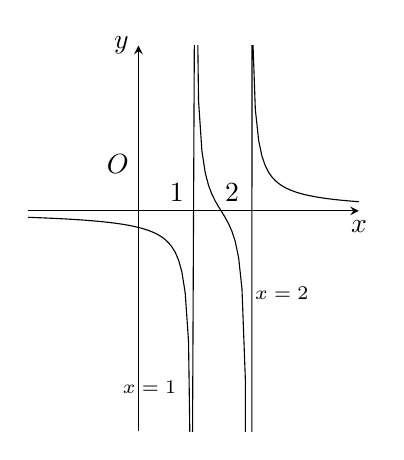
\begin{tikzpicture}[>=stealth,scale=0.7]
		\draw[->]  (-2,0) --(4,0);
		\draw[->](0,-4)--(0,3); 
		\draw (0,0.5)  node[above left]{$O$};
		\draw (4,0) node[below]{$x$}; 
		 \draw (0,3) node[left]{$y$};
		\draw (1,0) node[above left]{$1$}; 
		\draw (2,0) node[above  left]{$2$};
		\clip (-2,-4)  rectangle (4,3);
		\draw[samples=100]  plot[domain=-2:4]
			(\x,{(2*(\x)-3)/(5*(\x)^(2)-15*\x+10)}); 
		\draw (2.6,-1.5) node {\scriptsize  $x=2$};
		 \draw (0.2,-3.2) node {\scriptsize $x=1$};
	\end{tikzpicture}
		} 
	\loigiai{Dựa vào đồ thị hàm số ta thấy phương trình hai tiệm cận đứng là $x=1$ và $x=2$.\\ 
		Mặt khác đồ thị hàm số có đường tiệm  cận ngang là đường thẳng $y=0$.\\
		Vậy đồ thị là của hàm số $\dfrac{2x -  3}{5x^2-15x+10}$.
	 }
\end{ex}

% nguồn: Phan1_Lop_12_Dai_so_Chuong_1
\begin{ex}%[2D1H3-1]%[ma:5c0a0a30]
	Cho hàm số $y=\dfrac{x-m}{x+1}$ với $m$ là số thực. Tìm tất cả các giá trị của $m$ để tổng giá trị lớn nhất và giá trị nhỏ nhất của hàm số đã cho trên $[0; 2]$ bằng  $6$.
	\choice 
		{$m=4$} 
		 {\True $m=-4$}
		 {$m=1$}
		{$m=-1$} 
	\loigiai{Ta có  $y'=\dfrac{1+m}{(x+1)^2}$ nên hàm số luôn đồng biến hoặc nghịch biến trên $[0;2]$.\\
		Tổng giá trị lớn  nhất và nhỏ nhất của hàm số trên đoạn $[0; 2]$ bằng $6$ khi\\
	$y(0)+y(2)=6 \Leftrightarrow-m+\dfrac{2-m}{3}=6  \Leftrightarrow m=-4$.}
\end{ex}

% nguồn: Phan1_Lop_12_Dai_so_Chuong_1
\begin{ex}%[2D1H3-1]%[ma:f02d1e5d]
	\immini 
	{Bảng biến thiên sau là của đồ thị hàm số  nào sau đây?
	} 
	{
\begin{tikzpicture}
		\tkzTabInit[nocadre,lgt=1.5,espcl=3,deltacl=.5] 
			{$x$/0.7,$f’(x)$/0.7,$f  (x)$/2}
			{$-\infty$,$1$,$+\infty$} 
		 \tkzTabLine{,-,d,-,}
		\tkzTabVar{+/$+\infty$,-D+/  $-\infty$/$+\infty$,-/$-\infty$}
	\end{tikzpicture}
	} 
	 \choice
		 {$y = \dfrac{x+1}{x-1}$}
		{\True $y  = \dfrac{-x^2+2x}{x-1}$}
		{$y = \dfrac{-x^2+x}{x-1}$} 
		{$y =  \dfrac{x+2}{2x-2}$}
	\loigiai{Do $\lim\limits_{x \to 1^+} y = +\infty$  nên đồ thị có tiệm cận đứng là đường thẳng $x=1$.\\
		 Mặt khác $\lim\limits_{x \to +\infty} f(x) = -\infty$ và $\lim\limits_{x \to -\infty} f(x) = +\infty$ nên đồ thị hàm số không có tiệm cận ngang.\\
		Mặt khác  $y = \dfrac{-x^2+x}{x-1} = \dfrac{-1}{x-1}$ nên $\lim\limits_{x \to +\infty} \dfrac{-1}{x-1} = 0$.\\
		Vậy bảng  biến thiên của hàm số $y = \dfrac{-x^2+2x}{x-1}$.
	 }
\end{ex}

% nguồn: Phan1_Lop_12_Dai_so_Chuong_1
\begin{ex}%[2D1H3-1]%[ma:28a3bf6f]
	Giá trị lớn nhất của hàm số $y=x+\cos  ^2x$ trên $\left[0;\dfrac{\pi}{2} \right]$ là
	 \choice
		 {\True $\dfrac{\pi}{2}$}
		 {$\dfrac{\pi}{2}+1$}
		{$1$} 
		{$\dfrac{\pi}{4}+\dfrac{1}{2}$} 
	 \loigiai{
		Ta có: $y=f(x)=x+\cos  ^2x$ trên $\left[0;\dfrac{\pi}{2} \right]$.\\
		$y'=f'(x)=1-2\sin x\cdot \cos x=1-\sin 2x\ge 0$ với mọi $x \in \left[0;\dfrac{\pi}{2} \right]$.\\ 
		Suy ra $\displaystyle \max \limits_{\left[0;\tfrac{\pi}{2} \right]}  f(x) = f \left( \dfrac{\pi }{2}\right)=\dfrac{\pi}{2}$.
	} 
\end{ex}

% nguồn: Phan1_Lop_12_Dai_so_Chuong_1
\begin{ex}%[2D1H3-1]%[ma:035823d4]
	Cho hàm số  $y=f(x)$ có đạo hàm $f'(x)=(2x-1)(x+1)\left(x^2-1\right)$. Hàm số $y=f(x)$ có giá trị lớn nhất trên $[-2;1]$ bằng
	\choice 
		 {$f(-2)$}
		 {$f(-1)$}
		 {\True $f\left(\dfrac{1}{2}\right)$}
		 {$f(1)$}
	 \loigiai{
		Ta  có bảng biến thiên
		\begin{center}
			
\begin{tikzpicture}
				 \tkzTabInit[lgt=1.2,espcl=2.5]
					 {$x$ /1,$f’(x)$ /.7,$f (x)$ /2.5}
					 {$-2$,$-1$,$\dfrac{1}{2}$,$1$}
				 \tkzTabLine{,+,z,+,z,-,}
				\tkzTabVar{-/$-\infty$,R,+/$f\left(\dfrac{1}{2}\right)$,-/$-\infty$} 
			\end{tikzpicture}
		\end{center}
		Từ bảng  biến thiên của $y=f(x)$ ta thấy có giá trị lớn nhất của trên $[-2;1]$ bằng $f\left(\dfrac{1}{2}\right)$.
	 }
\end{ex}

% nguồn: Phan1_Lop_12_Dai_so_Chuong_1
\begin{ex}%[2D1H3-1]%[ma:dbbae84c]
	\immini{Cho hàm số $y=f(x)$ liên tục  trên $\mathbb{R}$ và $y=f'(x)$ có đồ thị như bên dưới. Giá trị lớn nhất của hàm số $y=f(x)$ trên đoạn $[0;3]$ là
	 \choice
		{\True  $f(0)$}
		 {$0$}
		 {$-4$}
		 {$f(2)$}}{
		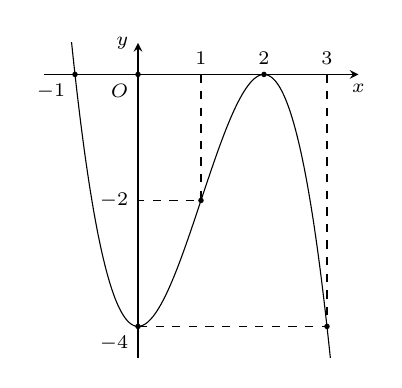
\begin{tikzpicture}[>=stealth,x=1cm,y=1cm,scale=.8]
			 \def\a{-1}
			 \def\b{3}
			 \def\c{0}
			 \def\d{-4}
			\draw[->] (-1.5,0) --  (3.5,0) node[below]{\scriptsize $x$};
			\draw[->] (0,-4.5) -- (0,.5) node[left] {\scriptsize  $y$};
			\draw[dashed] (0,0) node[below  left]{\scriptsize $O$}
				(-1,0) node[below  left]{\scriptsize $-1$}
				(1,0) node[above]{\scriptsize $1$}|-(0,-2) node[left]{\scriptsize $-2$} 
				(2,0) node[above]{\scriptsize  $2$}
				(3,0) node[above]{\scriptsize $3$}|-(0,-4) node[below left]{\scriptsize  $-4$};
			 \clip (-1.5,-4.5) rectangle (3.5,.5);
			\draw[samples=150,smooth,domain=-5:5]  plot (\x,{\a*(\x)^3+(\b)*(\x)^2+(\c)*\x+(\d)});
			\fill (0,0)  circle (1.25pt);
			\fill (-1,0)  circle (1.25pt);
			\fill (1,-2) circle  (1.25pt);
			\fill (2,0) circle  (1.25pt);
			\fill  (0,-4) circle (1.25pt);
			\fill (3,-4) circle (1.25pt); 
		\end{tikzpicture}
		} 
	\loigiai{ 
		Từ bảng biến  thiên
		ta thấy $f'(x)\leq0$ $\forall x\in(0;3)$ suy ra giá  trị lớn nhất của hàm số $y=f(x)$ trên đoạn $[0;3]$ là $f(0)$.
	} 
\end{ex}

% nguồn: Phan1_Lop_12_Dai_so_Chuong_1
\begin{ex}%[2D1H3-1]%[ma:782bd0db]
	Tìm giá trị thực của tham số $a$ để hàm số $f(x)=-x^3-3 x^2+a$ có giá trị nhỏ  nhất trên đoạn $[-1; 1]$ bằng 0.
	\choice 
		{$a=2$} 
		 {$a=6$}
		{$a=0$} 
		{\True $a=4$} 
	\loigiai{Xét hàm số $f(x)=-x^3-3 x^2+a$ trên  $[-1; 1]$, có $f'(x)=-3 x^2-6 x.$\\
		Phương trình $f'(x)=0 \Leftrightarrow  \heva{&-1 \leq x \leq 1 \\& -3 x^2-6 x=0} \Rightarrow x=0$.\\
		Tính $f(-1)=-2+a;  f(0)=a; f(1)=-4+a.$\\
		Suy ra $\min \limits_{[-1:  1]} f(x)=f(1)=-4+a=0 \Rightarrow a=4$.
	} 
\end{ex}

% nguồn: Phan1_Lop_12_Dai_so_Chuong_1
\begin{ex}%[2D1H3-1]%[ma:799aaf1b]
	Tiệm cận xiên của đồ thị hàm số $f(x)  = \dfrac{x^2+x-1}{x}$ là đường thẳng
	\choice 
		 {$y=x-1$}
		 {$y=x-2$}
		{$y=x-3$} 
		 {\True$y=x+1$}
	\loigiai{Gọi đường thẳng $y=ax+b, a\neq 0$ là đường tiệm cận xiên của hàm  số\\
		Ta có $a=\displaystyle\lim_{x\to +\infty  }\dfrac{\dfrac{x^2+x-1}{x}}{x}=1$.;
		$b=\displaystyle\lim_{x\to  +\infty }\left[\dfrac{x^2+x-1}{x}-x \right]=1$.\\
		Vậy đường tiệm cận  xiên cần tìm của đồ thị hàm số $f(x)$ có phương trình $y=x+1$.
	 }
\end{ex}

% nguồn: Phan1_Lop_12_Dai_so_Chuong_1
\begin{ex}%[2D1H3-1]%[ma:51c859ab]
	Giá trị nhỏ nhất của hàm số $y=x^3-3x+5$ trên đoạn $[2;4]$ là 
	\choice 
		{$5$} 
		 {$0$}
		{$3$} 
		{\True $7$} 
	 \loigiai{
		 Ta có $y=x^3-3x+5\Rightarrow y'=3x^2-3$.\\
		Giải $y'=  0\Leftrightarrow 3x^2-3=0\Leftrightarrow\hoac{&x=1\notin [2;4]\\&x=-1\notin [2;4].}$\\
		Do  đó, ta có
		$\heva{ 
		 &y(2)=8-6+5=7\\
		&y(4)=64-12+5=57. 
		}$\\ 
		 Suy ra $\min\limits_{[2;4]}y=y(2)=7$.
	} 
\end{ex}

% nguồn: Phan1_Lop_12_Dai_so_Chuong_1
\begin{ex}%[2D1H3-1]%[ma:59e5b200]
	\immini{ 
	Cho hàm số $y=f(x)$ liên tục trên $\mathbb{R}$ và có đồ thị như hình bên. Gọi $m,M$ lần lượt là giá trị nhỏ nhất và giá trị lớn nhất của hàm số $f(x)$ trên đoạn  $[-2;2]$. Phát biểu nào sau đây là đúng?
	 \choice
		{$m=-2$,  $M=2$}
		 {$m=1$, $M=3$}
		 {$m=3$, $M=1$}
		{\True $m=-1$, $M=3$} 
		}{\resizebox{!}{5cm}{\begin{tikzpicture}[line join=round,line cap=round,>=stealth]
		\draw[->]  (-2.5,0)--(3,0) node[below]{$x$};
		\draw[->] (0,-2.0)--(0,4.5)  node[left]{$y$};
		\draw[samples=100,domain=-2.1:2.1]  plot (\x,{-(\x)^3+3*(\x)+1});
		\draw (0,0) node[below  right]{$O$};
		\draw[dashed] 
			(-1,0)  node[above]{$-1$}
			 (0,1) node[left]{$1$}
			 (0,-1) node[right]{$-1$}
			(-2,0)  node[above left]{$-2$}
			(0,3) node[above left]{$3$} 
			 (1,0) node[below right]{$1$}
			(2,0) node[below right]{$2$} 
			 (1,0)--(1,3)--(0,3)
			(-1,0)--(-1,-1)--(0,-1); 
		 \fill (2,0) circle (1pt);
		 \fill (0,1) circle (1pt);
		 \fill (1,3) circle (1pt);
		\fill (-1,-1)  circle (1pt);
		\fill (-2,0) circle (1pt); 
		\fill (0,0)  circle (1pt);
	\end{tikzpicture}
		 }
		} 
	 \loigiai{
		Dựa vào đồ thị ta thấy hàm số trên đoạn $[-2;2]$, giá trị nhỏ nhất của  hàm số $f(x)$ bằng $-1$ tại $x=-1$, giá trị lớn nhất của hàm số $f(x)$ bằng $3$ tại $x=1$.
	 }
\end{ex}

% nguồn: Phan1_Lop_12_Dai_so_Chuong_1
\begin{ex}%[2D1H3-1]%[ma:73f5f17f]
	Cho hàm số $y=f(x)$ xác định, liên tục trên $\mathbb{R}$ và có đạo hàm $y=f'(x)$. Biết rằng hàm  số $y=f'(x)$ có đồ thị như hình vẽ bên.
	\begin{center}
		\begin{tikzpicture}[scale=1,font=\footnotesize,line join=round,line cap=round,>=stealth]
			\draw[->]  (-4,0)--(2,0) node[below left] {$x$};
			 \draw[->] (0,-3)--(0,3) node[below left] {$y$};
			\draw (0,0) node [above  right] {$O$};
			\foreach \x/\g in {-3/-150,-2/-150,-1/-90} 
			\fill (\x,0) circle  (1pt) node[shift={(\g:4mm)}] {\scriptsize $\x$};
			\foreach \y/\g  in {1/0,2/0}
			 \fill (0,\y) circle (1pt);
			\begin{scope}
				\clip (-4,-3)  rectangle (1,3);
				\draw[smooth,samples=200,domain=-3.2:0.5,smooth,variable=\x] plot  (\x,{-1*((\x)^4)-5*((\x)^3)-6*((\x)^2)});
			\end{scope}
		\end{tikzpicture}
	\end{center}
	Giá trị lớn nhất của hàm số $y=f(x)$ trên đoạn $[-3;1]$ là 
	\choice 
		{\True  $f(-2)$}
		{$f(-3)$} 
		 {$f(0)$}
		{$f(x_0)$ với $-3 < x_0 <  -2$}
	\loigiai{ 
		Ta có $f'(x) = 0 \Leftrightarrow \hoac{&x=-3\\&x=-2\\&x=0}$, với $x=-3$  và $x=-2$ là nghiệm bội lẻ, $x=0$ là nghiệm bội chẵn.\\
		Bảng biến thiên 
		\begin{center}
			
\begin{tikzpicture}
				\tkzTabInit 
					{$x$/0.7,$f'(x)$/0.7,$f  (x)$/2.5}{$-\infty$,$-3$,$-2$,$0$,$+\infty$}
				 \tkzTabLine{,-,0,+,0,-,0,-,}
				\tkzTabVar{+/$+\infty$,-/$f (-3)$,+/$f  (-2)$,R/,-/$-\infty$}
				\tkzTabIma{3}{5}{4}{$f  (0)$}
			\end{tikzpicture}
		\end{center}
		Vậy giá trị  lớn nhất của hàm số $y=f(x)$ trên đoạn $[-3;1]$ là $f(-2)$.
	} 
\end{ex}

% nguồn: Phan1_Lop_12_Dai_so_Chuong_1
\begin{ex}%[2D1H3-1]%[ma:4f435928]
	Giá trị nhỏ nhất của hàm  số $y=2 \cos ^3 x-\dfrac{9}{2} \cos ^2 x+3 \cos x+\dfrac{1}{2}$ là
	\choice 
		{$-9$} 
		{\True $1$} 
		 {$-\dfrac{3}{2}$}
		 {$\dfrac{1}{2}$}
	\loigiai{Đặt $t=\cos x \in[-1; 1]$, khi đó $y=f(t)=2 t^3-\dfrac{9}{2} t^2+3 t+\dfrac{1}{2}, -1 \leq t  \leq 1$.\\
		Xét hàm số $f(t)=2 t^3-\dfrac{9}{2} t^2+3 t+\dfrac{1}{2}$ trên $[-1; 1]$, có $f'(t)=8 t^2-9 t+3>0,  \forall t\in[-1; 1]$.\\
		Suy ra $f(t)$ là hàm số đồng biến trên $(-1; 1) \Rightarrow  \min \limits _{[-1; 1]} f(t)=f(-1)=1.$
	 }
\end{ex}

% nguồn: Phan1_Lop_12_Dai_so_Chuong_1
\begin{ex}%[2D1V3-1]%[ma:84c6d54f]
	Cho hàm số $f(x)=\dfrac{x-m^{2}}{x+4}$. Gọi $m_{0}$ là giá trị lớn nhất của tham số $m$ để hàm số đã cho có giá trị nhỏ nhất trên đoạn $[0; 6]$  bằng $-4$. Khẳng định nào sau đây đúng?
	 \choice
		 {$m_{0} \in(5; 7)$}
		{$m_{0}  \in(1; 3)$}
		{$m_{0} \in(7; 9)$} 
		{\True $m_{0} \in(3; 5)$} 
	 \loigiai{
		Ta  có $f(x)=\dfrac{x-m^{2}}{x+4} \Rightarrow f'(x)=\dfrac{m^{2}+4}{(x+4)^{2}}>0, \forall m$.\\
		Hàm số đồng biến trên $[0; 6]$.\\ 
	Suy ra $\min\limits_{[0; 6]}  f(x)=f(0)=-\dfrac{m^{2}}{4}=-4 \Leftrightarrow m^{2}=16 \Leftrightarrow m= \pm 4$ suy ra $m=4$.}
\end{ex}

% nguồn: Phan1_Lop_12_Dai_so_Chuong_1
\begin{ex}%[2D1V3-1]%[ma:30839286]
	Biết giá trị  lớn nhất của hàm số $y=x+\sqrt{4-x^2}+m$ là $3\sqrt{2}$. Giá trị của $m$ là
	\choice 
		 {$m=2\sqrt{2}$}
		{$m=-\sqrt{2}$} 
		{$m=\dfrac{\sqrt{2}}{2}$} 
		 {\True $m=\sqrt{2}$}
	\loigiai{ 
		Điều kiện xác  định: $-2\le x\le 2$.\\
		Ta có: $y=x+\sqrt{4-x^2}+m\Rightarrow  y'=1+\dfrac{-x}{\sqrt{4-x^2}} \Rightarrow y'=0\Leftrightarrow \sqrt{4-x^2}=x$.\\
		\[\Leftrightarrow \heva{&x\ge 0 \\ &4-x^2=x^2} \Leftrightarrow \heva{&x\ge 0 \\  &x^2=2} \Leftrightarrow x=\sqrt{2}\]
		Ta có  $y(-2)= -2+m$; $y(2)=2+m$; $y\left(\sqrt{2}\right)=2\sqrt{2}+m$.\\
		Vậy giá trị lớn nhất của hàm số  là $3\sqrt{2}$ $\Leftrightarrow 2\sqrt{2}+m=3\sqrt{2} \Leftrightarrow m=\sqrt{2}$.
	 }
\end{ex}

% nguồn: Phan1_Lop_12_Dai_so_Chuong_1
\begin{ex}%[2D1V3-1]%[ma:0f157baf]
	Cho hàm số $f(x)=x^3-3x+m$. Biết ${\mathop{\max}\limits_{\left(-\infty;0\right)}} f(x)=5$. Giá trị nhỏ nhất của hàm số $y=f(x)$ trên $\left(0;+\infty  \right)$ là
	 \choice
		{\True  ${\mathop{\min}\limits_{\left(0;+\infty \right)}} f(x)=1$}
		 {${\mathop{\min}\limits_{\left(0;+\infty \right)}} f(x)=2$}
		 {${\mathop{\min}\limits_{\left(0;+\infty \right)}} f(x)=3$}
		{${\mathop{\min}\limits_{\left(0;+\infty  \right)}} f(x)=-1$}
	\loigiai{ 
		Xét trên khoảng $\left(-\infty;0\right)$ có  $f'(x)=3x^2-3\Rightarrow f'(x)=0\Leftrightarrow x=1$ hoặc $x=-1$.\\
		 Bảng biến thiên:
		\begin{center}
			
\begin{tikzpicture}
				\tkzTabInit 
					[lgt=2,espcl=4] 
					{$x$/0.8,$f’(x)$/0.8,$f (x)$/2} 
					{$-\infty$,$-1$,$  0$}
				 \tkzTabLine{,+,0,-,}
				\tkzTabVar{-/  $-\infty$,+/ $2 +m$,-/$m$}
			\end{tikzpicture}
		\end{center}
		Khi đó ta có ${\mathop{\max}\limits_{\left(-\infty;0\right)}} f(x)=5\Leftrightarrow m+2=5\Leftrightarrow m=3\Rightarrow  f(x)=x^3-3x+3$.\\
		Xét  trên khoảng $\left(0;+\infty \right)$.\\ Bảng biến thiên
		\begin{center}
			
\begin{tikzpicture}
				\tkzTabInit 
					 [lgt=2,espcl=4]
					 {$x$/0.8,$f’(x)$/0.8,$f (x)$/2}
					{$  0 $,$1$,$ + \infty$}
				 \tkzTabLine{,-,0,+,}
				 \tkzTabVar{+/ $3$,-/ $1$,+/$+\infty$}
			\end{tikzpicture}
		\end{center}
		Vậy  ${\mathop{\min}\limits_{\left(0;+\infty \right)}} f(x)=1$.
	} 
\end{ex}

% nguồn: Phan1_Lop_12_Dai_so_Chuong_1
\begin{ex}%[2D1V3-1]%[ma:843f2131]
	Cho hàm số $f(x)=\dfrac{x-m^2}{x+8}$ với $m$ là tham số thực. Tìm giá trị lớn nhất của $m$ để hàm số có giá trị  nhỏ nhất trên đoạn $[0; 3]$ bằng $-2$.
	\choice 
		 {$m=-4$}
		 {$m=5$}
		{\True  $m=4$}
		{$m=1$} 
	\loigiai{ 
		 Xét hàm số $f(x)=\dfrac{x-m^2}{x+8}$ trên $[0; 3]$, có $f'(x)=\dfrac{8+m^2}{(x+8)^2}>0 , \forall x \in[0; 3]$\\
		 Suy ra $f(x)$ là hàm số đồng biến trên $(0; 3) \Rightarrow \min \limits _{[0; 3]} f(x)=f(0)=-\dfrac{m^2}{8}$\\
		Theo bài ta, ta có $\min \limits _{[0; 3]} f(x)=-2 \Leftrightarrow-\dfrac{m^2}{8}=-2 \Leftrightarrow m^2=16 \Rightarrow m_{\max  }=4$.
	} 
\end{ex}

% nguồn: Phan1_Lop_12_Dai_so_Chuong_1
\begin{ex}%[2D1V3-1]%[ma:5bf782f2]
	Biết rằng đồ thị hàm số $y =  \dfrac{(a - 3)x + a + 2025}{x - (b + 3)}$ nhận trục hoành làm tiệm cận ngang và trục tung làm tiệm cận đứng. Khi đó giá của $a + b$ là
	 \choice
		{$3$} 
		{$-3$} 
		{\True  $0$}
		{$6$} 
	\loigiai{Ta có $\heva{&\lim\limits_{x \to +\infty} \dfrac{(a-3)x + a + 2025}{x-(b+3)} =a-3&\\&\lim\limits_{x \to -\infty}\dfrac{(a-3)x+a+2025}{x-(b+3)}  = a - 3.}$\\
		Mặt khác $\heva{&\lim\limits_{x\to (b+3)^-} \dfrac{(a-3)x+a+2025}{x-(b+3)} = +\infty\\&\lim\limits_{x \to (b+3)^+} \dfrac{(a-3)x+a+2025}{x-(b+3)} = -\infty.}$\\ 
		Suy ra đồ thị hàm số có tiệm cận ngang là đường  thẳng $y=a-3$, tiệm cận đứng là đường thẳng $x=b+3$.\\
		Theo bài ra, ta có $\heva{&a -3 =0 \\&b + 3 = 0} \Rightarrow  \heva{&a = 3\\&b = -3} \Rightarrow a+b=0$.
	} 
\end{ex}

% nguồn: Phan1_Lop_12_Dai_so_Chuong_1
\begin{ex}%[2D1V3-1]%[ma:81ae365f]
	 Đồ thị hàm số $y = \dfrac{2x}{\sqrt{x^2-1}}$ có số đường tiệm cận là
	 \choice
		{$2$} 
		 {$1$}
		{$3$} 
		{\True$4$} 
	\loigiai{Ta có $\lim\limits_{x\to +\infty }\dfrac{2x}{\sqrt{x^2-1}} = \lim\limits_{x\to +\infty }\dfrac{2x}{|x|\sqrt{1-\dfrac{1}x^2}} =  \lim\limits_{x\to +\infty }\dfrac{2x}{x\sqrt{1-\dfrac{1}x^2}} = \lim\limits_{x\to +\infty }\dfrac{2}{\sqrt{1-\dfrac{1}x^2}}=2$.\\
		$\lim\limits_{x\to -\infty }\dfrac{2x}{\sqrt{x^2-1}}=\lim\limits_{x\to -\infty} \dfrac{2x}{|x|\sqrt{1-\dfrac{1}x^2}} = \lim\limits_{x\to -\infty} \dfrac{2x}{-x\sqrt{1-\dfrac{1}x^2}} =  \lim\limits_{x\to -\infty} \dfrac{-2}{\sqrt{1-\dfrac{1}x^2}}=-2$.\\
		Suy ra $y=-2$ và $y=2$ là phương trình  hai đường tiệm cận ngang của đồ thị hàm số đã cho.\\
		Mặt khác $\lim\limits_{x\to 1^-} y =  \lim\limits_{x\to (-1)^-} \dfrac{2x}{\sqrt{x^2-1}} = -\infty$; $\lim\limits_{x\to 1^+}y = \lim\limits_{x\to 1^+} \dfrac{2x}{\sqrt{x^2-1}} = +\infty$.\\
		Nên đồ thị hàm số có hai tiệm  cận đứng là đường thẳng $x=-1$ và đường thẳng $x=1$.\\
		 Vậy đồ thị hàm số có $4$ tiệm cận.
	 }
\end{ex}

% nguồn: Phan1_Lop_12_Dai_so_Chuong_1
\begin{ex}%[2D1V3-1]%[ma:915e71cf]
	Cho hàm số $y=\dfrac{x-m^2-2}{x-m}$, với $m$ là tham số. Gọi $S$ là tập các giá trị của $m$ để giá trị lớn  nhất của hàm số đã cho trên đoạn $[0;4]$ bằng $-1$. Tổng tất cả các phần tử của $S$ bằng
	\choice 
		{$-6$} 
		{$-1$} 
		 {$1$}
		{\True $-3$} 
	 \loigiai{
		Ta có  $y'=\dfrac{m^2-m+2}{(x-m)^2}>0$, $\forall x\ne m$.\\
		Suy  ra $\max\limits_{[0;4]}y=-1\Leftrightarrow \heva{&y(4)=-1\\&m\notin [0;4]}\Leftrightarrow\heva{&m^2+m-6=0\\&\hoac{&m>4\\&m<0}}\Leftrightarrow\heva{&\hoac{&m=2\\&m=-3}\\&\hoac{&m>4\\&m<0}}\Leftrightarrow m=-3$.\\
		Khi  đó $S=\{-3\}$. Vậy tổng tất cả các phần tử của $S$ bằng $-3$.
	 }
\end{ex}

% nguồn: Phan1_Lop_12_Dai_so_Chuong_1
\begin{ex}%[2D1V3-1]%[ma:ed140223]
	Cho hàm số $y=f(x)$ có bảng xét dấu đạo hàm  như sau:
	\begin{center}
		
\begin{tikzpicture}[>=stealth]
			\tkzTabInit[nocadre=false,lgt=1.2,espcl=2,deltacl=0.5] 
				{$x$/.7,$f'(x)$/.7} 
				 {$-\infty$,$-3$,$-2$,$-1$,$0$,$1$,$+\infty$}
			\tkzTabLine{,+,$0$,+,$0$,-,$0$,+,$0$,-,$0$,-,} 
		\end{tikzpicture}
	\end{center}
	Biết $f(-2)=f(0)=-3$. Giá trị lớn nhất của hàm số $y=\left|f(x)\right|$  trên đoạn $[-2;0]$ bằng
	\choice 
		 {$f(-1)$}
		 {$-3$}
		{\True  $-f(-1)$}
		{$3$} 
	 \loigiai{
		Dựa vào bảng dấu của đạo hàm, ta có bảng  biến thiên của $f(x)$ và từ đó suy ra bảng biến thiên của $\left|f(x)\right|$ như sau
		\begin{center}
			\begin{tikzpicture}[>=stealth]
				\tkzTabInit[nocadre=false,lgt=1.4,espcl=2,deltacl=0.5] 
					{$x$/.7,$f'(x)$/.7,$f (x)$/2,$\left|f (x)\right|$/2} 
					{$-\infty$,$-3$,$-2$,$-1$,$0$,$1$,$+\infty$} 
				\tkzTabLine{,+,$0$,+,$0$,-,$0$,+,$0$,-,$0$,-,} 
				\node at  ($(N32)-(0,0.3)$)
					(A)  {$-3$};
				 \node at ($(N43)+(0,0.3)$)
					 (B) {$f (-1)$};
				\node at ($(N52)-(0,0.3)$) 
					(C)  {$-3$};
				\node at ($(N34)+(0,0.3)$) 
					(D) {$3$}; 
				\node at ($(N54)+(0,0.3)$) 
					(E) {$3$}; 
				\node  at ($(N43)-(0,0.3)$)
					 (F) {$-f (-1)$};
				 \draw[->] ($(N13)+(0,0.2)$)--(A);
				\draw[->]  (A)--(B);
				\draw[->]  (B)--(C);
				\draw[->]  (C)--($(N73)+(0,0.2)$);
				 \draw[->] ($(N13)-(0,0.2)$)--(D);
				\draw[->] (D)--(F); 
				\draw[->] (F)--(E); 
				 \draw[->] (E)--($(N73)-(0,0.2)$);
			\end{tikzpicture}
		\end{center}
		 Do đó
		$$\max\limits_{[-2;0]}\left|f(x)\right|=\left|f(-1)\right|=-f(-1).$$ 
	} 
\end{ex}

% nguồn: Phan1_Lop_12_Dai_so_Chuong_1
\begin{ex}%[2D1V3-1]%[ma:2ff26b76]
	Gọi $M$, $m$  lần lượt là giá trị lớn nhất, giá trị nhỏ nhất của hàm số $y =x\sqrt{16-x^2}$. Tính $M+m$.
	 \choice
		{$8-\sqrt{8}$} 
		 {\True $0$}
		{$\sqrt{8}$} 
		{$8$} 
	\loigiai{ 
		Điều  kiện xác định $-4\le x\le 4$.\\
		Đạo  hàm $y'=\sqrt{16-x^2}-\dfrac{x^2}{\sqrt{16-x^2}}=\dfrac{16-2x^2}{\sqrt{16-x^2}}$.\\
		Suy ra $y'=0\Leftrightarrow  16-2x^2=0\Leftrightarrow\hoac{
		 &x=\sqrt{8}\in[-4;4]\\
		&x=-\sqrt{8}\in[-4;4]. 
		}$\\ 
		Ta có 
		$\heva{ 
		&y(-4)=y(4)=0\\ 
		 &y(-\sqrt{8})=-8\\
		 &y(\sqrt{8})=8.}$\\
		Do đó $M=8$,  $m=-8$ nên $M+m=0$.
	} 
\end{ex}

% nguồn: Phan1_Lop_12_Dai_so_Chuong_1
\begin{ex}%[2D1V3-1]%[ma:f6e15fdc]
	Cho hàm số $y=\left(x+m\right)^3-3\left(x+m\right)+1+n$. Biết hàm  số nghịch biến trên khoảng $\left(0;2\right)$ và giá trị lớn nhất của hàm số trên $\left[-1;1\right]$ bằng $4$. Tính $m+n$.
	 \choice
		{\True $m+n=0$} 
		 {$m+n=2$}
		{$m+n=-1$} 
		{$m+n=1$} 
	\loigiai{ 
		Ta  có: $y'=3\left(x+m\right)^2-3=3\left(x+m+1\right)\left(x+m-1\right)$.\\
		Giải phương trình  $y'=0\Leftrightarrow \hoac{&x=1-m\\&x=-1-m.}$\\
		 Bảng biến thiên.\\
		\begin{center}
			
\begin{tikzpicture}
				\tkzTabInit 
					[lgt=1.5,espcl=2] 
					{$x$/1.2,$f’(x)$/1} 
					 {$-\infty$,$-m-1$,$-m+1$,$+\infty$}
				 \tkzTabLine{,+,0,-,0,+,}
			\end{tikzpicture}
		\end{center}
		Hàm số nghịch biến trên $\left(0;2\right)$  khi
		$$-m-1 \le 0 < 2\le -m+1 \Leftrightarrow \heva{& m\ge -1 \\&  m \le -1} \Leftrightarrow m=-1.$$\\
		Với $m=-1$ thì $y'=0\Leftrightarrow \hoac{&x=0\in \left[-1;1\right] \\  &x=2\notin \left[-1;1\right].}$\\
		Ta có $y(0)=n+3; \, y(1)=n+1; \, y\left(-1\right)=n-1\Rightarrow {\mathop{\max}\limits_{\left[-1;1\right]}} y=n+3=4\Rightarrow n=1$.\\ 
		Vậy $ m+n=0$. 
	 }
\end{ex}

% nguồn: Phan1_Lop_12_Dai_so_Chuong_1
\begin{ex}%[2D1V3-1]%[ma:f40b2df9]
	 Giá trị lớn nhất của hàm số $y=2\cos x-\dfrac{4}{3}\cos^3x$ trên $[0;\pi]$ bằng
	\choice 
		{$\max\limits_{[0;\pi]}y=\dfrac{2}{3}$} 
		 {$\max\limits_{[0;\pi]}y=\dfrac{10}{3}$}
		{\True  $\max\limits_{[0;\pi]}y=\dfrac{2\sqrt{2}}{3}$}
		 {$\max\limits_{[0;\pi]}y=0$}
	\loigiai{ 
		Đặt $t=\cos  x\Rightarrow t\in[-1;1]$.\\
		Ta  được hàm $f(t)=2t-\dfrac{4}{3}t^3$.\\
		Khi đó  $f'(t)=2-4t^2=0\Leftrightarrow\hoac{
		 &t=\dfrac{1}{\sqrt{2}}\in[-1;1]\\
		&t=\dfrac{-1}{\sqrt{2}}\in[-1;1]. 
		}$\\ 
		 Ta được
		 $\heva{
		&f\left(-1\right)=-\dfrac{2}{3}\\ 
		&f\left(\dfrac{1}{\sqrt{2}}\right)=\dfrac{2\sqrt{2}}{3}\\ 
		&f\left(-\dfrac{1}{\sqrt{2}}\right)=\dfrac{-2\sqrt{2}}{3}\\ 
		&f(1)=\dfrac{2}{3}. 
		}$\\ 
		Vậy $\max\limits_{[0;\pi]}y=\max\limits_{[-1;1]}f(t)=\dfrac{2\sqrt{2}}{3}$. 
	} 
\end{ex}

% nguồn: Phan1_Lop_12_Dai_so_Chuong_1
\begin{ex}%[2D1V3-1]%[ma:cd452dd1]
	Cho hàm số $f(x)$ có đạo hàm $f'(x)=(x+1)(x-1)^2(x-2)$.  Giá trị nhỏ nhất của hàm số $g(x)=f(x)+\dfrac{1}{3} x^3-x-2$ trên đoạn $[-1; 2]$ bằng
	\choice 
		 {$f(2)-\dfrac{4}{3}$}
		{\True  $f(1)-\dfrac{8}{3}$}
		 {$f(0)-2$}
		{$f(-1)-\dfrac{4}{3}$} 
	 \loigiai{
		Ta  có $g'(x)=f'(x)+x^2-1$.\\
		 Khi đó $g'(x)=0 \Leftrightarrow(x+1)(x-1)^2(x-2)+x^2-1=0 \\
		\Leftrightarrow\left(x^2-1\right)\left(x^2-3  x+3\right)=0 \Leftrightarrow x= \pm 1$.\\
		 Do phương trình $x^2-3 x+3=0$ vô nghiệm.\\
		Bảng  biến thiên
		\begin{center}
			
\begin{tikzpicture}
				 \tkzTabInit[nocadre=false,lgt=1.5,espcl=2.1,deltacl=0.7]
					{$x$ /0.7,$g'(x)$ /0.7,$g (x)$ /2} 
					{$-1$,$1$,$2$} 
				 \tkzTabLine{,-,$0$,+,}
				\tkzTabVar{+/$ $,-/$g (1)$,+/$  $}
			\end{tikzpicture}
		\end{center}
	 Hàm số đạt giá trị nhỏ nhất tại $x=1$ và GTNN bằng $g(1)=f(1)-\dfrac{8}{3}$.}
\end{ex}

% nguồn: Phan1_Lop_12_Dai_so_Chuong_1
\begin{ex}%[2D1V3-1]%[ma:46cacfae]
	Cho hàm số $f(x)=\sqrt{2x+14}+\sqrt{5-x}$. Mệnh đề nào sau  đây đúng?
	 \choice
		{Hàm số đạt giá trị lớn nhất tại  $x=-7$}
		{Hàm số  đạt giá trị lớn nhất bằng $2\sqrt{6}$}
		{Hàm số  đạt giá trị nhỏ nhất tại $x=1$}
		{\True Hàm số đạt  giá trị nhỏ nhất bằng $2\sqrt{3}$}
	\loigiai{ 
		Tập xác định  $\mathscr{D}=[-7;5]$.\\
		 Ta có $f'(x)=\dfrac{1}{\sqrt{2x+14}}-\dfrac{1}{2\sqrt{5-x}}$.\\
		Suy ra $y'=0\Leftrightarrow\sqrt{2x+14}=2\sqrt{5-x}\Leftrightarrow  x=1$ $(\text{nhận})$.\\
		Ta được 
		 $\heva{
		 &f(1)=6\\
		&f(-7)=\sqrt{2\cdot(-7)+14}+\sqrt{5-(-7)}=0+\sqrt{12}=2\sqrt{3}\\ 
		 &f(5)=\sqrt{24}+0=2\sqrt{6}.
		 }$\\
		 Suy ra
		$$\max\limits_{[-7;5]}f(x)=6\text{ và }\min\limits_{[-7;5]}f(x)=2\sqrt{3}.$$ 
		 Vậy hàm số đạt giá trị nhỏ nhất bằng $2\sqrt{3}$.
	} 
\end{ex}

% nguồn: Phan1_Lop_12_Dai_so_Chuong_1
\begin{ex}%[2D1V3-1]%[ma:8083fc64]
	Cho hàm số $y=\dfrac{x+m}{x-1}$ ($m$ là tham số thực). Gọi  $m_0$ là giá trị của $m$ thỏa mãn ${\mathop{\min}\limits_{\left[2;4\right]}} y=3$. Mệnh đề nào dưới đây đúng?
	 \choice
		{$m_0  <-1$}
		{\True $m_0 > 4$} 
		{$1\le  m_0 < 3$}
		{$3<  m_0 \le 4$}
	 \loigiai{
		Ta có: $y'=\dfrac{-m-1}{\left(x-1\right)^2}$.\\ 
		 Nếu $-m-1> 0\Leftrightarrow m <-1$.\\
		Suy ra $ y' >  0$. Khi đó hàm số đã cho đồng biến trên $\left[2;4\right]$ nên ${\mathop{\min}\limits_{\left[2;4\right]}} y=y(2)=m+2$.\\
		Theo  giả thiết: $m+2=3\Leftrightarrow m=1$ (loại).\\
		Nếu $-m-1<  0\Leftrightarrow m >-1$
		$\Rightarrow y' <  0\Rightarrow$ hàm số đã cho nghịch biến trên $\left[2;4\right]$.\\ Suy ra ${\mathop{\min}\limits_{\left[2;4\right]}} y=y(4)=\dfrac{4+m}{3}$.\\
		Theo giả thiết:  $\dfrac{m+4}{3}=3\Leftrightarrow m=5$. Vậy $m_0=5$.
	 }
\end{ex}

% nguồn: Phan1_Lop_12_Dai_so_Chuong_1
\begin{ex}%[2D1V3-1]%[ma:bdec7374]
	 Tìm tất cả các giá trị thực của tham số $m$ để giá trị nhỏ nhất của hàm số $y=-x^3-3x^2+m$ trên đoạn $\left[-1;2\right]$ bằng $1$.
	\choice 
		 {$m=20$}
		{$m=19$} 
		 {$m=18$}
		{\True $m=21$} 
	 \loigiai{
		 Hàm số $y=-x^3-3x^2+m$ liên tục trên đoạn $\left[-1;2\right]$ và $y'=-3x^2-6x$.\\
		Ta có: $y'=0\Leftrightarrow \hoac{&x=0\in \left[-1;2\right]\\ &x=-2\notin \left[-1;2\right].}$\\ 
		$y\left(-1\right)=m-2;\,  y(0)=m;\, y(2)=m-20.$\\
		Suy  ra: ${\mathop{\min}\limits_{x\in \left[-1;2\right]}} y=1\Leftrightarrow m-20=1\Leftrightarrow m=21$.
	 }
\end{ex}

% nguồn: Phan1_Lop_12_Dai_so_Chuong_1
\begin{ex}%[2D1V3-1]%[ma:3fa6af95]
	Cho hàm số $y=x+\cos  ^2x+m$ ($m$ là tham số). Với giá trị nào của tham số $m$ thì ${\mathop{\min}\limits_{\left[0;\dfrac{\pi}{4} \right]}} y=4$?
	\choice 
		 {\True $m=3$}
		 {$m=\dfrac{3}{4}$}
		{$m=\dfrac{5}{2}$} 
		{$m=0$} 
	 \loigiai{
		Ta có: $y'=1-2\sin  x\cdot \cos x=1-\sin 2x\ge 0$, $\forall x\in \mathbb{R}$.\\
		 Khi đó ${\mathop{\min}\limits_{\left[0;\dfrac{\pi}{4} \right]}} y=y(0)=1+m=4$ $\Leftrightarrow m=3$.
	 }
\end{ex}

% nguồn: Phan1_Lop_12_Dai_so_Chuong_1
\begin{ex}%[2D1V3-1]%[ma:deec5a80]
	Giao điểm của hai đường tiệm cận của đồ thị hàm  số nào dưới đây nằm trên đường thẳng $d\colon y = x$?
	\choice 
		{$y = \dfrac{2x-1}{x+3}$} 
		{\True$y = \dfrac{x+4}{x-1}$} 
		{$y  = \dfrac{2x+1}{x+2}$}
		{$y =  \dfrac{1}{x+3}$}
	\loigiai{ 
		Đồ thị hàm  số $y = \dfrac{2x-1}{x+3}$ có giao điểm hai đường tiệm cận là $(-3; 2) \notin d$.\\
		Đồ thị hàm số $y = \dfrac{x+4}{x-1}$ có giao điểm hai đường tiệm cận là $(1;  1) \in d$.\\
		Đồ thị hàm số $y = \dfrac{2x+1}{x+2}$ có giao điểm hai đường  tiệm cận là $(-2; 2) \notin d$.\\
		Đồ thị hàm số $y = \dfrac{1}{x+3}$ có giao điểm hai đường tiệm cận là  $(-3; 0) \notin d$.\\
	} 
\end{ex}

% nguồn: Phan1_Lop_12_Dai_so_Chuong_1
\begin{ex}%[2D1V3-1]%[ma:b343ac87]
	Cho hàm số $f(x)=\dfrac{2x+m}{x-3}$ (với $m$ là tham số). Giá trị của $m$ để  ${\mathop{\max}\limits_{\left[-1;2\right]}} f(x)+{\mathop{\min}\limits_{\left[-1;2\right]}} f(x)=8$ là
	\choice 
		{$m=\dfrac{4}{5}$} 
		{\True  $m=-\dfrac{46}{5}$}
		{$m=-12$} 
		 {$m=\dfrac{18}{5}$}
	\loigiai{ 
		Ta có: $f'(x)=\dfrac{-6-m}{\left(x-3\right)^2}$.\\ 
		Nếu $m=-6\Rightarrow  y=2$. Khi đó $\displaystyle \max_{[-1;2]} f(x) + \displaystyle \min_{[-1;2]} f(x)=4 $ nên $m=-6$ loại.\\
		Nếu $m\ne-6$, khi  đó
		\begin{eqnarray*}
			&&{\mathop{\max}\limits_{\left[-1;2\right]}} f(x)+{\mathop{\min}\limits_{\left[-1;2\right]}}  f(x)=8
			 \\ &\Leftrightarrow & f\left(-1\right)+f(2)=8\\
			 &\Leftrightarrow & \dfrac{-2+m}{-4}+\dfrac{4+m}{-1}=8 \\
			&\Leftrightarrow  &m=-\dfrac{46}{5}.
	\end{eqnarray*} }
\end{ex}

% nguồn: Phan1_Lop_12_Dai_so_Chuong_1
\begin{ex}%[2D1V3-1]%[ma:9acc8e77]
	Gọi $m$, $M$ lần lượt  là giá trị nhỏ nhất và giá trị lớn nhất của hàm số $f(x)=\dfrac{1}{2}x-\sqrt{x+1}$ trên đoạn $[0;3]$. Tổng $S=2M-m$ bằng
	\choice 
		{\True  $S=0$}
		{$S=-\dfrac{3}{2}$} 
		 {$S=-2$}
		{$S=4$} 
	\loigiai{ 
		Hàm số $f(x)$  liên tục trên đoạn $[0;3]$.\\
		Ta có  $f(x)=\dfrac{1}{2}x-\sqrt{x+1}\Rightarrow f'(x)=\dfrac{1}{2}-\dfrac{1}{2\sqrt{x+1}}=\dfrac{\sqrt{x+1}-1}{2\sqrt{x+1}}$.\\
		 Giải phương trình $f'(x)=0\Leftrightarrow\sqrt{x+1}=1\Rightarrow x=0$.\\
		Xét các  giá trị
		 $\heva{
		 &f(0)=-1\\
		&f(3)=-\dfrac{1}{2}. 
		}$\\ 
		Suy ra 
		$M=-\dfrac{1}{2}$, $m =  -1$.\\
		Vậy  $S=2M-m=2\cdot\left(\dfrac{-1}{2}\right)-(-1)=0$.
	} 
\end{ex}

% nguồn: Phan1_Lop_12_Dai_so_Chuong_1
\begin{ex}%[2D1V3-1]%[ma:2d82c61e]
	Cho hàm số $f(x)=10^x+x$ và hàm số $g(x)=x^3-mx^2+\left(m^2+1\right)x-2$. Gọi $M$ là giá trị lớn nhất của hàm số $g\left(x+f(x)\right)$  trên đoạn $\left[0;1\right]$. Khi $M$ đạt giá trị nhỏ nhất thì giá trị của tham số $m$ bằng
	\choice 
		 {$\dfrac{21}{2}$}
		{\True  $6$}
		{$21$} 
		{$5$} 
	\loigiai{ 
		 Đặt $t=x+f(x)$ vì $x\in \left[0;1\right]\Rightarrow t\in \left[1;12\right]$.\\
		Xét $g(t)=t^3-mt^2+\left(m^2+1\right)t-2$  trên $\left[1;12\right]$.\\
		$\Rightarrow g'(t)=3t^2-2mt+m^2+1$ có $\Delta '=m^2-3\left(m^2+1\right)=-2m^2-3< 0 \, \forall  m$.\\
		$\Rightarrow g'(t)  > 0 \, \forall t\in \left[1;12\right]$ $\Rightarrow y=g(t)$ đồng biến trên $\left[1;12\right]$.\\
		Vậy $M={\mathop{\max}\limits_{t\in  \left[1;12\right]}} g(t)=g(12)=12m^2-144m+1738$.\\
		$\Rightarrow M$ đạt giá trị nhỏ nhất khi $m=\dfrac{144}{2\cdot  12}=6$.
	} 
\end{ex}

% nguồn: Phan1_Lop_12_Dai_so_Chuong_1
\begin{ex}%[2D1V3-1]%[ma:05ddc83c]
	Có  bao nhiêu giá trị nguyên của tham số $m$ để hàm số $y=\dfrac{x-m^2}{x+8}$ có giá trị nhỏ nhất trên $\left[0; 3\right]$ bằng $-\dfrac{9}{2}$?
	\choice 
		{$0$} 
		{\True  $2$}
		{$3$} 
		 {$1$}
	 \loigiai{
		Hàm số $y=\dfrac{x-m^2}{x+8}$ có tập xác  định $\mathscr D=\mathbb{R}\setminus \{-8\}$ nên hàm số xác định và liên tục trên đoạn $\left[0; 3\right]$.\\
		Ta có $y'=\dfrac{8+m^2}{\left(x+8\right)^2} > 0, \forall m\in \mathbb{R},x\ne-8$  nên hàm số đồng biến trên đoạn $\left[0; 3\right]$.\\
		Suy ra ${\mathop{\min}\limits_{\left[0; 3\right]}} y=y(0)=-\dfrac{m^2}{8}$.\\ Từ  giả thiết suy ra $-\dfrac{m^2}{8}=-\dfrac{9}{2} \Leftrightarrow m^2=36\Leftrightarrow \hoac{&m=6 \\ &m=-6.}$\\
		Vậy có hai giá trị nguyên của tham  số $m$ thoả mãn yêu cầu bài toán.
	} 
\end{ex}

% nguồn: Phan1_Lop_12_Dai_so_Chuong_1
\begin{ex}%[2D1V3-1]%[ma:462eae44]
	Hỏi tập hợp nào dưới đây chứa  tất cả các giá trị thực của tham số $m$ để giá trị lớn nhất của hàm số $y=\left|x^4-2 x^2+m\right|$ trên đoạn $[0; 2]$ bằng $5$?
	 \choice
		 {$(-\infty;-5) \cup(0;+\infty) $}
		 {\True $(-5;-2) $}
		 {$(-4;-1) \cup(5;+\infty) $}
		{$(-4;-3)  $}
	\loigiai{ 
		 Xét hàm số $f(x)=x^4-2 x^2+m$ trên $[0; 2]$.\\
		 Ta có $f'(x)=4 x^3-4 x$; $ f'(x)=0\Leftrightarrow
		 \hoac{&x=0 \\& x= \pm 1.}$\\
		Tính $|f(0)|=|m|;  |f(1)|=|m-1|; |f(2)|=|m+8|$.\\
		Suy ra  $\max \limits_{[1; 2]} y=\{|m-1|;|m+8|\}$
		\begin{itemize}
			\item Nếu $\max  \limits _{[1; 2]} y=|m-1| \text{ thì } \heva{|m-1|=5 \\ |m-1| \geq|m+8|} \Leftrightarrow m=-4 $.\\
			\item Nếu $\max \limits _{[1; 2]} y=|m+8| \text{  thì } \heva{|m+8|=5 \\ |m+8| \geq|m-1|}\Leftrightarrow m=-3$.\\
		\end{itemize}
	Vậy có  2 giá trị $m$ cần tìm và thuộc khoảng $(-5;-2) $.}
\end{ex}

% nguồn: Phan1_Lop_12_Dai_so_Chuong_1
\begin{ex}%[2D1V3-1]%[ma:2ec2290a]
	Cho hàm số $y=\left(x^{3}-3 x-m+1\right)^{2}$. Tổng tất cả các giá trị của tham số $m$ sao cho giá trị nhỏ nhất của hàm  số trên đoạn $[-1; 1]$ bằng $4$ là
	\choice 
		{\True $-2$} 
		 {$2$}
		{$-4$} 
		 {$4$}
	\loigiai{ 
		Đặt $t=g(x)=x^{3}-3 x+1$ là hàm số xác định và  liên tục trên đoạn $[-1; 1]$.\\
		Ta khảo sát hàm số $g(x)$ trên  đoạn $[-1; 1]$.\\
		Bảng  biến thiên của $g(x)$
		\begin{center}
			
\begin{tikzpicture}
				 \tkzTabInit[lgt=2,espcl=2]
					{$x$/1,$g'(x)$/1,$g  (x)$/2}
					 {$-\infty$,$-1$,$1$,$+\infty$}
				\tkzTabLine{,-,z,+,z,-,} 
				\tkzTabVar{+/$+\infty$,-/$-3$,+/$1$,-/$-\infty$} 
			\end{tikzpicture}
		\end{center}
		Từ bảng biến thiên ta thấy $x  \in[-1; 1]$ thì $t \in[-3; 1]$.\\
		Bài toán trở thành: Tìm $m$ để  hàm số $y=f(t)=(t-m)^{2}$ có giá trị nhỏ nhất của hàm số trên đoạn $[-3;1]$ bằng $4$.\\
		Ta có $f'(t)=2(t-m)=0 \Leftrightarrow t=m$.\\ 
		Nếu $m \in[-3; 1]$ thì $f(m)=0$, $f(-3)\ge 0$, $f(1)\ge 0$, suy ra $\min\limits_{[-3; 1]} f(t)=f(m)=0$, tức là không tồn tại  $m$ thỏa mãn yêu cầu bài toán.\\
		Nếu $m>1$ thì $f(1) = (1-m)^2=m^2 -2m+1$, $f(-3)=(-3-m)^2= m^2 +6m+9$.\\ 
		 Suy ra $\min\limits_{[-3; 1]} f(t)=f(1)=(1-m)^{2}$
		$\Leftrightarrow(1-m)^{2}=4\Leftrightarrow\hoac{&m-1=2  \\ &m-1=-2} \Leftrightarrow\hoac{&m=-1 \\ &m=3. }$\\
		Nếu $m<-3$  thì
		$f(1) = (1-m)^2=m^2 -2m+1$, $f(-3)=(-3-m)^2= m^2  +6m+9$.\\
		Suy ra  $f(-3) - f(1) = 8m+8<8\cdot (-3) + 8=-16<0$.\\
		Do  đó
		$\min\limits_{[-3;  1]} f(t)=f(-3)=(-3-m)^{2}$
		$\Leftrightarrow(-3-m)^{2}=4 \Leftrightarrow\hoac{&3+m=2 \\  &3+m=-2. }\Leftrightarrow\hoac{&m=-5 \\ &m=-1.}$\\
		Vậy có hai giá trị của $m$ thỏa  mãn yêu cầu bài toán: $m=3; m=-5$.\\
	Vậy tổng tất  cả các giá trị của $m$ là $-2$.}
\end{ex}


%%%%%%%%%%%%%%%% ĐÚNG/SAI %%%%%%%%%%%%%%%%

% nguồn: Phan1_Lop_12_Dai_so_Chuong_1
\begin{ex}%[2D1N3-1]%[ma:fc5b1e24]
	\immini{Cho  hàm số $f(x)=ax^3+bx^2+cx+d$ ($a$, $b$, $c$, $d\in \mathbb{R})$ có đồ thị như hình bên.
	\choiceTF 
		{\True Điểm cực  tiểu của hàm số là $0$}
		{Điểm cực đại của hàm số  là $4$}
		{Hàm số đồng biến trên khoảng  $(0;3)$}
		 {\True Giá trị lớn nhất của hàm số trên đoạn $[-1;3]$ bằng $4$}
		}{\resizebox{!}{5cm}{\begin{tikzpicture}[line join=round,line cap=round,>=stealth]
		 \tikzset{label style/.style={font=\footnotesize}}
		\draw[->] (-2.1,0)--(4.1,0)  node[below left] {$x$};
		\draw[->]  (0,-2.1)--(0,5.1) node[below left] {$y$};
		\fill (0,0)  node [below left] {$O$} circle (1pt);
		\foreach \x in {-2,-1,1,2} 
		 \draw (\x,2pt)--(\x,-1pt) node [below] {$\x$};
		\foreach \y in {-2,-1,1,2,3,4} 
		\draw (2pt,\y)--(-1pt,\y)  node [left] {$\y$};
		\begin{scope}
			\clip  (-2,-2) rectangle (4,5);
			\draw[samples=100,domain=-2:4,smooth,variable=\x] plot  (\x,{-((\x)^3)+3*((\x)^2)+0*(\x)+0});
		\end{scope}
		\fill (3,0) node  [below left] {$3$} circle (1pt);
	\end{tikzpicture}
		 }}
	 \loigiai{
		\begin{itemchoice}
			\itemch \textbf{Đúng}. Điểm cực  tiểu của hàm số đã cho là $x=0$.
			\itemch \textbf{Sai}. Điểm  cực đại của hàm số đã cho là $x=2$.
			\itemch \textbf{Sai}. Trên $(0;3)$ ta thấy hàm số đồng biến trên  khoảng $(0;2)$, nghịch biến trên khoảng $(2;3)$.
			\itemch \textbf{Đúng}. Giá trị lớn nhất của  hàm số trên đoạn $[-1;3]$ bằng $4$.
		\end{itemchoice}
	 }
\end{ex}

% nguồn: Phan1_Lop_12_Dai_so_Chuong_1
\begin{ex}%[2D1N3-1]%[ma:f20dd761]
	Cho hàm số $y=f(x)$ xác định trên tập $\mathscr{D}$. Số $M$ và $m$ lần lượt được gọi là giá trị lớn nhất và giá trị nhỏ nhất của  hàm số $y=f(x)$ trên $\mathscr{D}$.
	\choiceTF 
		{$f(x) \geq M$ với mọi $x \in \mathscr{D}$ thì $M$ là  GTLN của hàm số}
		{\True $m$ là GTNN nếu $f(x)\geq m$ với mọi $x \in \mathscr{D}$ và tồn tại $x_0 \in \mathscr{D}$  sao cho $f\left(x_0\right)=m$}
		 {$M-m=0$}
		{\True $M$ là GTLN nếu $f(x)\leq M$ với mọi  $x \in \mathscr{D}$ và tồn tại $x_0 \in \mathscr{D}$ sao cho $f\left(x_0\right)=M$}
	\loigiai{ 
		\begin{itemchoice}
			\itemch $M$ là GTLN nếu $f(x) \leq M$ với mọi $x \in \mathscr{D}$ và tồn tại $x_0 \in \mathscr{D}$ sao cho $f\left(x_0\right)=M$. 
			\itemch Số  $m$ được gọi là GTNN của hàm số $y=f(x)$ trên $\mathscr{D}$ nếu $f(x) \geq m$ với mọi $x \in \mathscr{D}$ và tồn tại $x_0 \in \mathscr{D}$ sao cho $f\left(x_0\right)=m$.
			\itemch $M-m=a$, với $a$ là số  thực.
			\itemch Số $M$ được gọi là GTLN của hàm số $y=f(x)$ trên $\mathscr{D}$ nếu $f(x)\leq M$ với mọi $x \in  \mathscr{D}$ và tồn tại $x_0 \in \mathscr{D}$ sao cho $f\left(x_0\right)=M$.
		\end{itemchoice}
	 }
\end{ex}

% nguồn: Phan1_Lop_12_Dai_so_Chuong_1
\begin{ex}%[2D1H3-1]%[ma:8f593e4a]
	Cho hàm số $y=f(x)$ liên tục trên ${\bf \mathbb{R}}$ và có  bảng biến thiên trong hình vẽ dưới đây:
	\begin{center}
		
\begin{tikzpicture}
			\tkzTabInit 
				 [lgt=1.5,espcl=2]
				{$x$/1.2,$f’(x)$/1,$f  (x)$/2}
				{$-\infty$,$-1$,$0$,$1$,$+\infty$} 
			\tkzTabLine{,+,0,-,0,+,0,-,} 
			\tkzTabVar{-/ $-\infty$,+/ $4 $,-/$3$,+/ $4 $,-/ $-\infty$} 
		\end{tikzpicture}
	\end{center}
	 \choiceTF
		{\True Cực đại của hàm  số là $4$}
		{\True Cực tiểu của hàm  số là $3$}
		 {\True ${\mathop{\max}\limits_{\mathbb{R}}} y=4$}
		{${\mathop{\min}\limits_{\mathbb{R}}} y=3$} 
	\loigiai{ 
		\begin{itemchoice}
			\itemch Cực  đại của hàm số là $4$
			\itemch Cực  tiểu của hàm số là $3$
			 \itemch ${\mathop{\max}\limits_{\mathbb{R}}} y=4$
			\itemch Từ bảng biến thiên ta thấy ${\mathop{\lim}\limits_{x\to+\infty}}f(x)=-\infty$ nên  hàm số không có giá trị nhỏ nhất trên $\mathbb{R}$.
		\end{itemchoice}
	} 
\end{ex}

% nguồn: Phan1_Lop_12_Dai_so_Chuong_1
\begin{ex}%[2D1H3-1]%[ma:e76a9af2]
	Hàm  số $y=f(x)$ liên tục trên đoạn $[-2;1]$ và có hình vẽ như sau.
	\begin{center}
		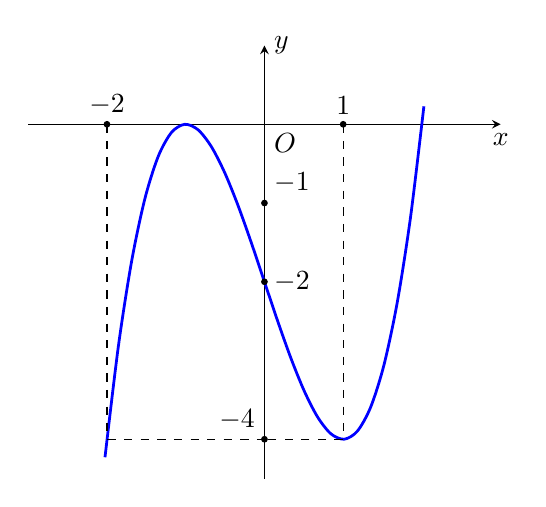
\begin{tikzpicture}[>=stealth]
			\draw[->]  (-3,0) --(0,0) node[below
				 right]{$O$} -- (3,0)
				 node[below]{$x$};
			\draw[->](0,-4.5)--(0,1) 
				 node[right]{$y$};
			\draw[smooth,blue,line width=1] 
				plot[domain=-2.025:2.025] 
				 (\x,{(\x)^(3)-3*(\x)-2});
			\draw[dashed](-2,0) 
				 node[above]{$-2$} -- (-2,-4) --
				(0,-4) node[above  left]{$-4$};
			\draw (0,-2) node[right]  {$-2$};
			\draw[dashed]  (1,0)
				 node[above]{$1$} -- (1,-4) --
				 (0,-4) node[above]{};
			\draw (0,-1)  node[above right] {$-1$};
			\draw[fill] (-2,0)  circle (1pt);
			 \draw[fill] (1,0) circle (1pt);
			\draw[fill] (0,-1) circle (1pt); 
			\draw[fill] (0,-2)  circle (1pt);
			\draw[fill] (0,-4) circle  (1pt);
		\end{tikzpicture}
	\end{center}
	Gọi $M$ và $m$ lần lượt là GTLN và  GTNN của hàm số trên $[-2;1]$.
	\choiceTF 
		 {\True $m=-4$}
		 {$M=-1$}
		{\True $M+m=-4$} 
		 {\True Hàm số đạt GTLN tại $x=-1$}
	 \loigiai{
		\begin{itemchoice}
			\itemch GTNN của hàm số trên $[-2;1]$ là  $m=-4$.
			\itemch GTLN  của hàm số trên $[-2;1]$ là $M=0$.
			\itemch $M+m=-4+0=-4$. 
			\itemch GTLN của hàm số trên $[-2;1]$ bằng $0$ tại  $x=-1$.
		\end{itemchoice}
	 }
\end{ex}

% nguồn: Phan1_Lop_12_Dai_so_Chuong_1
\begin{ex}%[2D1H3-1]%[ma:023ce939]
	\immini 
	{Hàm số $y=f(x)$  liên tục trên đoạn $[-1;3]$ và có bảng biến thiên như sau. Gọi $M$ và $m$ lần lượt là GTLN và GTNN của hàm số trên $[-1;3]$.
	\choiceTF 
		{$m=f(2)$} 
		 {$M=f(4)$}
		 {\True $m=f(-1)$}
		{\True  $M=f(0)$}}
		{
\begin{tikzpicture}
		 \tkzTabInit[nocadre=false,lgt=1.2,espcl=2]
			{$x$ /0.8,$y'$ /0.8,$y$ /2} 
			 {$-1$,$0$,$2$,$3$}
		\tkzTabLine{,+,$0$,-,$0$,+,} 
		\tkzTabVar{-/$0$,+/$5$,-/$1$,+/$4$} 
	\end{tikzpicture}
		} 
	\loigiai{	\begin{itemchoice}
		\itemch Dựa vào bảng biến thiên ta  có $m=f(-1)$.
		\itemch  Dựa vào bảng biến thiên ta có $M=f(0)$.
		\itemch Dựa vào bảng  biến thiên ta có $m=f(-1)$.
		\itemch Dựa vào bảng biến  thiên ta có $M=f(0)$.
\end{itemchoice}}
\end{ex}

% nguồn: Phan1_Lop_12_Dai_so_Chuong_1
\begin{ex}%[2D1H3-1]%[ma:ca935c5a]
	Cho hàm số  $f(x) = \sin2x - x$.
	 \choiceTF
		 {$f\left(-\dfrac{\pi}{2}\right) = \dfrac{\pi}{2}, \quad f\left(\dfrac{\pi}{2}\right) = -\dfrac{\pi}{2}
		$} 
		{\True Đạo hàm  của hàm số là~$y'=\cos 2x-1$}
		{Nghiệm của phương trình $f'(x) = 0$ trên  đoạn $\left[-\dfrac{\pi}{2}; \dfrac{\pi}{2}\right]$ phương trình có nghiệm là~$x = -\dfrac{\pi}{6}; x = \dfrac{\pi}{6}$}
		{\True Giá trị nhỏ nhất của $f(x)$  trên đoạn $\left[-\dfrac{\pi}{2}; \dfrac{\pi}{2}\right]$ là~$f(x) = -\dfrac{\pi}{2}$}
	\loigiai{\begin{itemchoice}
		 \itemch \textbf{Đúng}.\\
		$f\left(-\dfrac{\pi}{2}\right) =  \sin(-\pi) - \left(-\dfrac{\pi}{2}\right) = \sin(-\pi) + \dfrac{\pi}{2} = \sin\pi + \dfrac{\pi}{2} = \dfrac{\pi}{2}
		$. 
		 \itemch \textbf{Sai}.\\
		Đạo hàm của hàm số  $f'(x) = 2\cos(2x) - 1$.
		\itemch  \textbf{Đúng}.\\
		 $f'(x) = 2\cos(2x) - 1 = 0$\\
		$  \Leftrightarrow \cos(2x) = \dfrac{1}{2}$\\
		$\Leftrightarrow x = -\dfrac{\pi}{6}$; $x = \dfrac{\pi}{6}$ là~nghiệm trên đoạn $\left[-\dfrac{\pi}{2}; \dfrac{\pi}{2}\right]$. 
		 \itemch \textbf{Đúng}.\\
		Nghiệm $x = \pm\dfrac{\pi}{6}$ thuộc  đoạn $\left[-\dfrac{\pi}{2}; \dfrac{\pi}{2}\right]$.
		\[ 
		f\left(-\dfrac{\pi}{2}\right) = \dfrac{\pi}{2}, \quad f\left(\frac{\pi}{2}\right)  = -\dfrac{\pi}{2}, \quad f\left(\dfrac{\pi}{6}\right) = \dfrac{\sqrt{3}}{2}-\dfrac{\pi}{6}
		, \quad f\left(-\dfrac{\pi}{6}\right) = -\dfrac{\sqrt{3}}{2}  + \dfrac{\pi}{6}.
		\] 
		Giá trị nhỏ nhất  là~$-\dfrac{\pi}{2}$.
	\end{itemchoice}
 }
\end{ex}

% nguồn: Phan1_Lop_12_Dai_so_Chuong_1
\begin{ex}%[2D1H3-1]%[ma:326ac91b]
	\immini 
	{Cho đồ thị của hàm số $f(x)$ như  hình bên.
	 \choiceTF
		{Đường thẳng $y=x+1$ là đường tiệm cận ngang của đồ thị hàm  số $f(x)$}
		 {\True Đồ thị hàm số $f(x)$ có một đường tiệm cận đứng và một đường tiệm cận xiên }
		{\True Hàm số có phương  trình là $f(x)=\dfrac{x^2+2x+2}{x+1}$}
		{\True Đồ thị hàm số $f(x)$  có đường tiệm cận xiên là đường thẳng $y=x+1$}
		 }
		{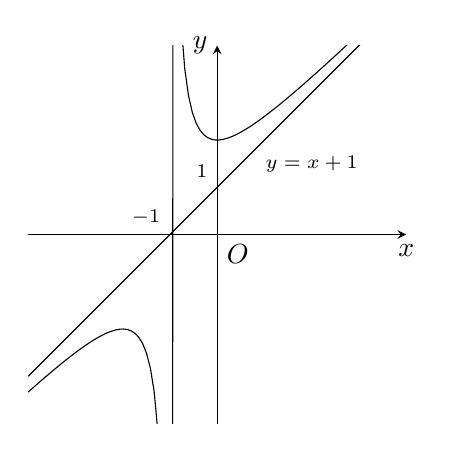
\begin{tikzpicture}[>=stealth,scale=0.6]
		\draw[->] (-4,0) --(4,0); 
		 \draw[->](0,-4)--(0,4);
		\draw (0,0)  node[below right]{$O$};
		\draw  (4,0) node[below]{$x$};
		\draw (0,4) node[left]{$y$}; 
		\draw  (-1,0) node[above left]{\scriptsize $-1$};
		\draw (0,1) node[above left]{\scriptsize $1$}; 
		\clip (-4,-4) rectangle  (4,4);
		\draw[samples=100] plot[domain=-4:4] 
			(\x,{((\x)^2+2*\x+2)/((\x)+1)}); 
		\draw[samples=100] plot[domain=-4:4] 
			 (\x,{\x+1});
		\draw (2,1.5)  node {\scriptsize $y=x+1$};
	\end{tikzpicture}
		} 
	 \loigiai{
		\begin{itemchoice}
			\itemch Dựa vào đồ thị hàm số của $f(x)$, đồ thị hàm số không có tiệm cận  ngang.
			\itemch Dựa vào đồ thị hàm số của $f(x)$, đồ thị hàm  số có đường tiệm cận đứng $x=-1$.
			\itemch Gọi $y=ax+b,a\neq0$ là phương trình đường tiệm  cận xiên của đồ thị hàm số $f(x)$.\\
			$a = \lim\limits_{x \to +\infty} \dfrac{f(x)}{x} = \lim\limits_{x \to +\infty} \dfrac{\dfrac{x^2+2x+2}{x+1}}{x} = \lim\limits_{x  \to +\infty} \dfrac{x^2+2x+2}{x(x+1)} = 1$.\\
			$b = \lim\limits_{x  \to +\infty}[f(x)-ax] = \lim\limits_{x \to +\infty} \left[\dfrac{x^2 + 2x + 2}{x + 1} - x\right]=1$.\\
			Vậy đường thẳng $y=x+1$ là  đường tiệm cận xiên của đồ thị hàm số $f(x)$.\\
			Ta có  $\heva{&\lim\limits_{x \to -1^+} \dfrac{x^2+2x+2}{x+1} = +\infty\\&
			\lim\limits_{x \to  -1^-} \dfrac{x^2+2x+2}{x+1}= -\infty.}$\\
			Vậy $x=-1$  là phương trình đường tiệm cận đứng.
			\itemch  Dựa vào đồ thị, đường thẳng $y=x+1$ là đường tiệm cận xiên của đồ thị hàm số $f(x)$.
		\end{itemchoice}
	 }
\end{ex}

% nguồn: Phan1_Lop_12_Dai_so_Chuong_1
\begin{ex}%[2D1H3-1]%[2H2V2-6]%[ma:e5b9aa15]
	Một máy bay đang di chuyển về phía sân bay. Tại thời điểm hiện tại,  vị trí của máy bay là~$B(150;150;5\,000)$ (trong đó $5\,000$ m là~độ cao của máy bay so với mặt đất). Máy bay đang di chuyển thẳng tới sân bay với vận tốc $700$ km/h. Sân bay có tọa độ $C(0;0;0)$ và máy bay đang tiến dần đến vị trí hạ cánh tại sân bay.
	 \choiceTF
		{Phương trình tham số của đường thẳng mà máy bay di chuyển theo là~$\begin{cases}
		x =  150 - 150t \\
		y  = 150 - 150t \\
		z  = 5\,000 - 5\,000t
\end{cases}
$} 
{Khoảng cách từ vị trí hiện  tại của máy bay $B(150;150;5\,000)$ đến sân bay $C(0;0;0)$ là~$\sqrt{15\,250\,000} \approx 3\,905{,}6 \, \text{ km}$}
{Với vận tốc của  máy bay là~$700$ km/h, thời gian để máy bay hạ cánh là~khoảng $5{,}5$ giờ}
{\True Nếu hệ thống kiểm soát không lưu yêu cầu liên lạc với máy bay khi nó còn cách sân bay $40$ km, thì khi máy bay ở vị trí $(6;6;200)$ (đơn vị m) nó  còn cách sân bay là~$40$ km}
\loigiai{\begin{itemchoice}
	\itemch  \textbf{Đúng}.\\
	Véc tơ chỉ phương của đường thẳng $BC$ là~$\overrightarrow{BC} = (-150; -150; -5000)$ nên phương trình tham số của đường  thẳng là
	\[ 
	\begin{cases}
		x = 150 - 150t\\ 
		y =  150 - 150t\\
		 z = 5\,000 - 5\,000t.
	\end{cases}
	 \]
	 \itemch \textbf{Sai}.\\
	Khoảng cách từ điểm $B(150; 150; 5\,000)$ đến $C(0; 0; 0)$ được  tính như sau:
	 \[
	\text{ d}_{BC} = \sqrt{(150 - 0)^2  + (150 - 0)^2 + (5\,000 - 0)^2} = \sqrt{25\,045\,000}\approx 5\text{ (km)}.
	\] 
	\itemch \textbf{Sai}.\\ 
	Thời gian hạ cánh khi máy bay di chuyển  với vận tốc $700$ km/h được tính là~$t = \dfrac{5{,}0}{700}\text{ (h)}$.
	\itemch  \textbf{Sai}.\\
	Khoảng cách từ điểm $(6;6;200)$ đến  $(0;0;0)$ được tính như sau
	\[ 
	d = \sqrt{(6 - 0)^2 + (6 - 0)^2 + (200 - 0)^2} = \sqrt{40\,072}\approx 200{,}18\text{ (m)}. 
	 \]
	\end{itemchoice}
} 
\end{ex}

% nguồn: Phan1_Lop_12_Dai_so_Chuong_1
\begin{ex}%[2D1H3-1]%[ma:6117d01e]
	Cho hàm số $y=\dfrac{x-m^{2}-2}{x-m}$,  với $m$ là tham số. Khi đó
	\choiceTF 
		{Tập xác  định của hàm số là $\mathscr{D}=\mathbb{R}$}
		{\True Khi $m=1$ thì hàm số  đồng biến trên mỗi khoảng $(-\infty; 1)$ và $(1;+\infty)$}
		{Khi $m=1$ thì trên đoạn  $[1; 4]$ hàm số đạt giá trị lớn nhất bằng $\dfrac{1}{2}$}
		{Có duy nhất 1 giá trị của tham số $m$ để giá  trị lớn nhất của hàm số trên đoạn $[0; 4]$ bằng $-1$}
	\loigiai{\begin{itemchoice}
		\itemch Tập xác định của  hàm số là $\mathscr{D}=\mathbb{R} \setminus\{m\}$.
		\itemch Khi $m=1$  thì $y=\dfrac{x-3}{x-1}$.\\
		Ta có $y'=\dfrac{2}{(x-1)^{2}}>0$ nên hàm số đồng biến trên mỗi  khoảng $(-\infty; 1)$ và $(1;+\infty)$.
		\itemch Khi $m=1$  thì trên đoạn $[1; 4]$ hàm số đạt giá trị lớn nhất bằng $f(4)=\dfrac{1}{3}$.
		\itemch Có duy nhất $1$ giá trị của tham số $m$ để giá trị lớn nhất của hàm số trên đoạn $[0; 4]$ bằng  $-1$.\\
		Ta có hàm số đạt giá trị lớn nhất  trên $[0; 4]$ bằng $-1$ khi \\
		$\heva{&m\notin [0;4] \\ &f(4)=-1}\Leftrightarrow \heva{&\hoac{&m<0\\ &m>4}  \\ &\dfrac{2-m^{2}}{4-m}=-1} \Leftrightarrow\heva{&\hoac{&m<0\\ &m>4}\\ &m^{2}+m-6=0} \Leftrightarrow\heva{&\hoac{&m<0\\ &m>4}\\ &\hoac{&m=2\\&m=-3}}\Leftrightarrow m=-3$.
\end{itemchoice}}
\end{ex}

% nguồn: Phan1_Lop_12_Dai_so_Chuong_1
\begin{ex}%[2D1H3-1]%[ma:a7cf000c]
	Cho hàm số $y=\dfrac{x^2+mx-1}{x+m}$,  với $m$ là tham số thực dương
	 \choiceTF
		{Tập  xác định của hàm số là $\mathscr{D}=\mathbb{R}$}
		{Trên đoạn $[2;4]$ thì đạo hàm của hàm số  luôn nhận giá trị dương}
		{Giá trị  nhỏ nhất của hàm số trên đoạn $[2;4]$ là $\min\limits_{[2;4]}y=y(2)$}
		{\True Chỉ có duy nhất một giá trị  của tham số $m$ để $\min\limits_{[2;4]}y=\dfrac{9}{5}$}
	\loigiai{ 
		\begin{itemchoice}
			\itemch Tập xác định  của hàm số là $\mathscr{D}=\mathbb{R}\setminus\{-m\}$.
			\itemch Lấy $m=-2$ ta có $y=\dfrac{x^2+3x-1}{x-2}$thấy hàm số  không xác định tại $x=2$. Do đó hàm số không có đạo hàm tại $x=2$.
			\itemch 
			Lấy $m=-2$ ta có $y=\dfrac{x^2+3x-1}{x-2}$thấy hàm  số không xác định tại $x=2$. Do đó hàm số không có giá trị nhỏ nhất tại $x=2$.
			\itemch Với $-m\notin [2;4]$. Ta  có $y' = \dfrac{(x+m)^2+1}{(x+m)^2}>0$.\\
			Suy ra $\min\limits_{[2;4]}y=\dfrac{9}{5}\Leftrightarrow \heva{&y(2)=\dfrac{2m+3}{m+2}=\dfrac{9}{5}\\&-m\notin [2;4]}\Leftrightarrow \heva{&m=3\\ &\hoac{&m<-4\\&m>-2}}\Leftrightarrow m=3$.\\ 
			Chỉ có duy nhất một giá trị của tham số $m$ để $\min\limits_{[2;4]}y=\dfrac{9}{5}$  là $m=3$.
	\end{itemchoice}}
\end{ex}

% nguồn: Phan1_Lop_12_Dai_so_Chuong_1
\begin{ex}%[2D1H3-1]%[ma:726bf6ec]
	Cho hàm số $y =  \dfrac{3(x^2+1)(x-3)}{(x+1)^3}$.
	 \choiceTF
		{Đồ thị hàm số không  có tiệm cận ngang}
		{\True Đồ thị hàm  số có đúng một tiệm cận ngang}
		{Đồ thị hàm số có một tiệm cận xiên} 
		{Đồ  thị hàm số không có tiệm cận đứng}
	 \loigiai{
		\begin{itemchoice}
			\itemch Ta có $\lim\limits_{x \to \pm \infty} \dfrac{3(x^2+1)(x-3)}{(x+1)^3} = \lim\limits_{x \to \pm \infty} \dfrac{3\left(1+\dfrac{1}{x^2} \right) \left(1-\dfrac{3}{x} \right)}{1 + \dfrac{3}{x}  + \dfrac{3}{x^2} + \dfrac{1}{x^3}} = 3$.\\
			Đồ thị hàm số có đúng một tiệm cận  ngang $y=3$.
			\itemch Đồ thị hàm số có đúng một tiệm cận  ngang.
			\itemch Đồ thị hàm số có tiệm cận ngang  thì không có tiệm cận xiên.
			\itemch Ta có  $\heva{&\lim\limits_{x \to -1^-}\dfrac{3(x^2+1)(x-3)}{(x+1)^3} = +\infty\\&
			\lim\limits{x\to -1^+}\dfrac{3(x^2+1)(x-3)}{(x+1)^3}  = +\infty.}$\\
			Vậy Đồ thị hàm số có một tiệm cận đứng  $x=-1$.
		\end{itemchoice}
	} 
\end{ex}

% nguồn: Phan1_Lop_12_Dai_so_Chuong_1
\begin{ex}%[2D1H3-1]%[ma:c9a59cf9]
	\immini{Cho hàm số $y=f(x)$ có đạo hàm $y=f'(x)$ liên tục trên $\mathbb{R}$ và đồ thị hàm số $f'(x)$ như  hình vẽ bên.
	\choiceTF 
		{Hàm số có hai điểm  cực trị}
		{Hàm số  $y=f(x)$ đồng biến trên khoảng $\left(1;+\infty \right)$}
		{\True $f(1)  > f(2) > f(4)$}
		{\True Trên đoạn $\left[1; 4\right]$ thì giá trị lớn nhất của hàm số $f(x)$ là $f(1)$}}{\begin{tikzpicture}[line join = round,line cap = round,>=stealth,font=\footnotesize,scale=0.6]
		\def\xt{-2} \def\xp{6} \def\yd{-3}  \def\yt{4}
		 \draw[->] (\xt,0)--(\xp,0) node[below]{$x$};
		\draw[->] (0,\yd)--(0,\yt) node[left]{$y$}; 
		\fill (0,0)  circle (1.5pt) node[below left]{$O$};
		\begin{scope}
			\clip  (\xt+0.1,\yd+0.1) rectangle (\xp-0.1,\yt-0.1);
			\draw[samples=150,smooth,domain=-2:5]  plot (\x,{0.2*(\x-1)*(\x+1)*(\x-4)});
		\end{scope}
		\fill (1,0) circle  (1.5pt) node[above]{$1$}
			(4,0) circle  (1.5pt) node[below right]{$4$}
			(-1,0)  circle (1.5pt) node[above left]{$-1$};
	\end{tikzpicture}
		 }
	\loigiai{ 
		\begin{itemchoice}
			\itemch Ta có $f'(x)=0$ có ba nghiệm bội lẻ là $x=\pm  1$, $x=4$ nên hàm số $y=f(x)$ có ba điểm cực trị.
			\itemch Dựa vào đồ thị hàm số $y=f'(x)$, ta thấy hàm số $y= f(x)$ đồng biến trên hai khoảng  $(-1;1)$ và $(4; +\infty)$.
			\itemch Do hàm số nghịch biến trên đoạn $[1;4]$ mà $1<2< 4$  nên $f(1)> f(2)> f(4)$.
			\itemch Ta có hàm số nghịch biến trên $[1; a) $ và đồng biến trên $(a;  4]$ (với $a\in(1;4)$) nên $\displaystyle \max_{[1;4]} f(x)= f(4)$.
		\end{itemchoice}
	} 
\end{ex}

% nguồn: Phan1_Lop_12_Dai_so_Chuong_1
\begin{ex}%[2D1H3-1]%[ma:cda15038]
	Cho hàm số $y=m x+\dfrac{36}{x+1}$, với $m$  là tham số. Khi đó
	\choiceTF 
		{\True Hàm số đã cho nghịch biến trên đoạn $[0;  3]$ khi $m \leq 0$}
		{\True Khi $m \leq 0$ thì giá trị nhỏ nhất  của hàm số trên đoạn $[0; 3]$ là $3 m+9$}
		{\True Khi $\dfrac{9}{4} \leq m \leq 36$ thì giá trị nhỏ nhất của hàm số $y=m x+\dfrac{36}{x+1}$ trên $[0; 3]$ là  $-m+12 \sqrt{m}$}
		{\True Có đúng một giá  trị nguyên của tham số $m$ để giá trị nhỏ nhất của hàm số \break $y=m x+\dfrac{36}{x+1}$ trên $[0; 3]$ bằng $20$}
	 \loigiai{
		\begin{itemchoice}
			\itemch Ta có $y'=m-\dfrac{36}{(x+1)^{2}}$. Với $m<0$ ta có $y'<0$ do đó hàm  số đã cho nghịch biến trên đoạn $[0; 3]$ khi $m \leq 0$.
			\itemch Với $m \leq 0$, hàm số nghịch biến trên $[0;  3]$ nên $\min\limits_{x \in[0; 3]} y=y(3)=3 m+9$.
			\itemch Với $m>0$, ta có $y'=\dfrac{m(x+1)^{2}-36}{(x+1)^{2}}=0 \Leftrightarrow x+1= \pm  \dfrac{6}{\sqrt{m}} \Leftrightarrow\hoac{&x=-1+\dfrac{6}{\sqrt{m}} \\ &x=-1-\dfrac{6}{\sqrt{m}}~(\text {loại})}$.\\
			 Khi $0 \leq-1+\dfrac{6}{\sqrt{m}} \leq 3 \Leftrightarrow \dfrac{9}{4} \leq m \leq 36$, ta có bảng biến thiên của hàm số:
			\begin{center}
				
\begin{tikzpicture}
					\tkzTabInit[lgt=2,espcl=3] 
						{$x$/1,$y'(x)$/1,$y (x)$/2} 
						{$0$,$-1+\dfrac{6}{\sqrt{m}}$,$3$} 
					\tkzTabLine{,-,z,+,} 
					 \tkzTabVar{+/$36$,-/$-m+12\sqrt{m}$,+/$3m+9$}
				\end{tikzpicture}
			\end{center}
			Dựa vào bảng biến thiên ta suy ra  \\
			$\min\limits_{x  \in[0; 3]} y=y\left(-1+\dfrac{6}{\sqrt{m}}\right)=-m+12 \sqrt{m}$
			\itemch Với $m>0$, ta có $y^{\prime}=\dfrac{m(x+1)^{2}-36}{(x+1)^{2}}=0 \Leftrightarrow x+1= \pm \dfrac{6}{\sqrt{m}}  \Leftrightarrow\hoac{&x=-1+\dfrac{6}{\sqrt{m}} \\ &x=-1-\dfrac{6}{\sqrt{m}}~(\text {loại})}$.\\
			Khi $0 \leq-1+\dfrac{6}{\sqrt{m}} \leq 3 \Leftrightarrow \dfrac{9}{4} \leq  m \leq 36$, ta có bảng biến thiên của hàm số:
			\begin{center}
				
\begin{tikzpicture}
					\tkzTabInit[lgt=2,espcl=3] 
						{$x$/1,$y'(x)$/1,$y  (x)$/2}
						 {$0$,$-1+\dfrac{6}{\sqrt{m}}$,$3$}
					 \tkzTabLine{,-,z,+,}
					\tkzTabVar{+/$36$,-/$-m+12\sqrt{m}$,+/$3m+9$} 
				\end{tikzpicture}
			\end{center}
			Dựa vào bảng biến thiên ta suy  ra \\
			$\min\limits_{x \in[0; 3]} y=y\left(-1+\dfrac{6}{\sqrt{m}}\right)=-m+12 \sqrt{m}=20 \Leftrightarrow\hoac{&m=4  \\ &m=100~ (\text{loại})}$.\\
			Khi $-1+\dfrac{6}{\sqrt{m}}>3 \Leftrightarrow m<\dfrac{9}{4}$, ta có bảng biến thiên của hàm số: 
			\begin{center}
				
\begin{tikzpicture}
					 \tkzTabInit[lgt=2,espcl=3]
						{$x$/1,$y'(x)$/1,$y (x)$/2} 
						{$0$,$3$} 
					\tkzTabLine{,-,} 
					\tkzTabVar{+/$36$,-/$3m+9$} 
				\end{tikzpicture}
			\end{center}
			 Dựa vào bảng biến thiên ta suy ra $\min\limits_{x \in[0; 3]} y=y(3)=3 m+9=20 \Leftrightarrow m=\dfrac{11}{9}$ (loại).\\
			Vậy giá trị nhỏ nhất bằng  $20$ {khi} $m=4$.
		\end{itemchoice}
	 }
\end{ex}

% nguồn: Phan1_Lop_12_Dai_so_Chuong_1
\begin{ex}%[2D1H3-1]%[ma:cca5c187]
	\immini{Hình bên cho biết sự thay đổi của nhiệt độ ở một thành phố trong một ngày 
	\choiceTF 
		{Nhiệt độ cao nhất trong ngày là $28^{\circ} C$} 
		{\True Nhiệt độ thấp nhất  trong ngày là $20^{\circ} C$}
		 {\True Thời điểm nhiệt độ cao nhất trong ngày là lúc $16$ giờ}
		{\True Thời điểm nhiệt độ thấp nhất trong ngày là lúc $4$ giờ}}{\begin{tikzpicture}[scale=0.8,font=\footnotesize,line join=round,line cap=round]
		 \def\xmin{-0.5}\def\xmax{7}\def\ymin{-0.5}\def\ymax{6.5}
		\draw[->]  (\xmin-0.2,0)--(\xmax,0) node[above] {\footnotesize $x \text{ giờ}$};
		\draw[->] (0,\ymin-0.2)--(0,\ymax+0.2) node[right]  {\footnotesize $t \,(^\circ C)$};
		\fill (0.0,0.0) node[below right]{$O$} circle (1pt); 
		 \draw (0,4)..controls+(-40:0.15) and+(180:0.5)..(1,3)
			..controls+(0:0.9)  and+(180:0.5)..(2,5)
			..controls+(0:0.5)  and+(180:0.5)..(3,4.5)
			..controls+(0:0.5)  and+(180:0.5)..(4,6)
			..controls+ (0:0.5)  and+(135:0.35)..(5,4.3)
			..controls+(-45:0.15) and+(180:0.5)..(6,3.7); 
		\fill (1,0) circle  (1.5pt) node[below]{$4$}
			(2,0) node[below]{$8$} circle  (1.5pt)
			 (3,0) circle (1.5pt) node[below]{$12$}
			 (4,0) circle (1.5pt) node[below]{$16$}
			(5,0) circle  (1.5pt) node[below]{$20$}
			(6,0) circle (1.5pt) node[below]{$24$} 
			 (0,4) circle (1.5pt) node[above left]{$25$}
			(1,3) circle (1.5pt) node[above]{$20$} 
			(2,5) circle  (1.5pt) node[above]{$31$}
			(3,4.5)  circle (1.5pt) node[above]{$28$}
			(4,6) circle (1.5pt) node[above]{$34$} 
			(5,4.3) circle (1.5pt) node[above right]{$27$} 
			(6,3.7) circle  (1.5pt) node[above]{$24$};
		\draw[dashed] (1,0)--(1,3) 
			 (2,0)--(2,5)
			 (3,0)--(3,4.5)
			 (4,0)--(4,6)
			 (5,0)--(5,4.3)
			(6,0)--(6,3.7); 
	\end{tikzpicture}
		 }
	 \loigiai{
		\begin{itemchoice}
			\itemch Nhiệt độ  cao nhất trong ngày là $34^{\circ} C$
			\itemch Nhiệt độ  thấp nhất trong ngày là $20^{\circ} C$
			\itemch Thời điểm  nhiệt độ cao nhất trong ngày là lúc $16$ giờ
			\itemch Thời  điểm nhiệt độ thấp nhất trong ngày là lúc $4$ giờ
		\end{itemchoice}
	 }
\end{ex}

% nguồn: Phan1_Lop_12_Dai_so_Chuong_1
\begin{ex}%[2D1V3-1]%[ma:7188e388]
	Cho hàm  số $f(x)={\rm e}^{x^2-2 x}$.
	\choiceTF 
		 {$f'(x)=(x-1) {\rm e}^{x^2-2 x}$}
		{\True $f'(x)=0\Leftrightarrow  x=1$}
		 {$f(0)=\dfrac{1}{\rm e}, f(1)=0, f(2)=0$}
		{\True Giá trị nhỏ nhất của hàm số  $f(x)={\rm e}^{x^2-2 x}$ trên $[0; 2]$ là $\dfrac{1}{\rm e}$}
	\loigiai{ 
		Ta có $f'(x)=2(x-1)\mathrm{e}^{x^2-2x}$.\\ 
		$f'(x)=0\Leftrightarrow 2(x-1)\mathrm{e}^{x^2-2x}\Leftrightarrow  x-1=0\Leftrightarrow x=1$.\\
		$f(0)=1$;  $f(1)=\mathrm{e}^{-1}=\dfrac{1}{\mathrm{e}}$; $f(2)=0$.\\
		Ta có $\dfrac{1}{\mathrm{e}}<1$ nên giá trị nhỏ nhất của  hàm số $f(x)={\rm e}^{x^2-2 x}$ trên $[0; 2]$ là $\dfrac{1}{\rm e}$.
		\begin{itemchoice}
			\itemch Sai. $a$ có đúng 1 căn bậc  $n$ khi $n$ lẻ.
			 \itemch Đúng.
			\itemch  Đúng.
			\itemch  Đúng.
		\end{itemchoice}
	 }
\end{ex}

% nguồn: Phan1_Lop_12_Dai_so_Chuong_1
\begin{ex}%[2D1V3-1]%[ma:354bc032]
	Cho hàm số $f(x)=\cos 2x-x$. 
	 \choiceTF
		{\True $f\left(-\dfrac{\pi}{2}\right)=\dfrac{\pi}{2}-1$; $f\left(\dfrac{\pi}{2}\right)=-\dfrac{\pi}{2}-1$} 
		{Đạo hàm của hàm số đã cho là  $f'(x)=2\sin 2x-1$}
		{Phương trình $f'(x)=0$ có đúng hai nghiệm trên đoạn $\left[-\dfrac{\pi}{2}; \dfrac{\pi}{2}\right]$  là $x=-\dfrac{\pi}{12}$ và $x=\dfrac{5\pi}{12}$}
		{\True Giá trị nhỏ nhất  của hàm số $y=f(x)$ trên đoạn $\left[-\dfrac{\pi}{2}; \dfrac{\pi}{2}\right]$ là $-\dfrac{\pi}{2}-1$}
	\loigiai{ 
		\begin{itemchoice}
			\itemch  \textbf{Đúng}.\\
			$f\left(-\dfrac{\pi}{2}\right)=\cos (-\pi)+\dfrac{\pi}{2}=\dfrac{\pi}{2}-1$.\\ $f\left(\dfrac{\pi}{2}\right)=\cos (\pi)-\dfrac{\pi}{2}=-\dfrac{\pi}{2}-1$ 
			\itemch  \textbf{Sai}.\\
			Đạo hàm  của hàm số đã cho là $f'(x)=-2\sin 2x-1$.
			\itemch  \textbf{Sai}.\\
			Ta có $f'(x)=-2\sin 2x-1=0\Leftrightarrow \sin 2x=-\dfrac{1}{2}\Leftrightarrow  \hoac{&x=-\dfrac{\pi}{12}+k\pi\\&x=\dfrac{7\pi}{12}+k\pi}, k\in \mathbb{Z}$.\\
			Vì $x\in  \left[-\dfrac{\pi}{2}; \dfrac{\pi}{2}\right]$ nên $x\in \left\{-\dfrac{\pi}{12};-\dfrac{5\pi}{12}\right\}$.\\
			\itemch \textbf{Đúng}.\\ 
			Ta  có $f\left(-\dfrac{\pi}{2}\right)=\dfrac{\pi}{2}-1$.\\
			 $f\left(\dfrac{\pi}{2}\right)=-\dfrac{\pi}{2}-1$.\\
			$f\left(-\dfrac{\pi}{12}\right)=\dfrac{\pi}{12}+\dfrac{\sqrt{3}}{2}$.\\ 
			 $f\left(-\dfrac{5\pi}{12}\right)=\dfrac{5\pi}{12}-\dfrac{\sqrt{3}}{2}$.\\
			Vậy  giá trị nhỏ nhất của hàm số $y=f(x)$ trên đoạn $\left[-\dfrac{\pi}{2}; \dfrac{\pi}{2}\right]$ là $-\dfrac{\pi}{2}-1$.
		\end{itemchoice}
	 }
\end{ex}

% nguồn: Phan1_Lop_12_Dai_so_Chuong_1
\begin{ex}%[2D1V3-1]%[ma:05b062c5]
	Cho hàm số $y=f(x)$ có đạo  hàm liên tục trên $\mathbb{R}$. Hàm số $y=f'(x)$ có đồ thị như hình dưới đây.
	\begin{center}
		\begin{tikzpicture}[>=stealth]
			\draw [->] (-1.5,0) --  (4.8,0) node[below left]{$x$};
			\draw [->] (0,-2)  -- (0,2) node[below left]{$y$};
			 \foreach \x/\label in {-1/-1,1/1,4/4}
			\draw (\x,0.1) --  (\x,-0.1) node[below=2pt]{$\label$};
			\node  [below right=1pt and -1pt] at (0,0) {$O$};
			\draw[smooth,samples=100,domain=-1.6:4.5,variable=\x] 
				plot  (\x,{0.2*(\x+1)*(\x-1)*(\x-4)});
		\end{tikzpicture}
	\end{center}
	 \choiceTF
		{Hàm số $y=f(x)$ đồng biến  trên khoảng $(1;+\infty)$}
		 {\True Trên đoạn $\left[-1;4\right]$ thì giá trị lớn nhất của hàm số $y=f(x)$ là~$f(1)$}
		{\True $f(1) >  f(2) > f(4)$}
		{Hàm số $y=f(x)$ có hai cực  trị}
	\loigiai{ 
		Xét $f'(x)=0\Leftrightarrow \hoac{&{x=-1} \\ &{x=1}  \\&{x=4}}$. \\
		Bảng  biến thiên:
		\begin{center}
			\resizebox{0.8\linewidth}{!}{
\begin{tikzpicture}
		\tkzTabInit [nocadre,lgt=1.2,espcl=3] 
			{$x$/1.2,$f’(x)$/1.2,$f (x)$/2.5} 
			{$-\infty$,$-1$,$1$,$4$,$+\infty$} 
		 \tkzTabLine{,-,z,+,z,-,z,+,}
		\tkzTabVar{+/,-/,+/,-/,+/} 
	\end{tikzpicture}
			} 
		\end{center}
		\begin{itemchoice}
			\itemch Hàm số đồng biến trên  $(-1;1),(4;+\infty)$.
			 \itemch Từ bảng biến thiên, ta thấy giá trị lớn nhất của hàm số trên đoạn $\left[-1;4\right]$ là~$f(1)$.
			\itemch Vì  hàm số nghịch biến trên $(1;4)$ nên $f(1) > f(2) > f(4)$
			 \itemch Từ bảng biến thiên, ta thấy hàm số đã cho có ba điểm cực trị.
		\end{itemchoice}
	} 
\end{ex}

% nguồn: Phan1_Lop_12_Dai_so_Chuong_1
\begin{ex}%[2D1V3-1]%[ma:cb5b9f34]
	 Cho hàm số $f(x)=x^3-3x+m$, với $m$ là tham số
	 \choiceTF
		{Khi $m=0$ thì hàm số  đồng biến trên khoảng $(-1;1)$}
		 {\True Khi $m=0$ thì hàm số có hai điểm cực trị}
		{\True Giá trị nhỏ nhất của hàm số trên đoạn $[0;2]$  bằng $m-2$}
		{Gọi $S$ là tập tất cả các giá trị của tham số $m$ sao cho giá trị lớn nhất của hàm số $y=|f(x)|$ trên đoạn $[0;2]$ bằng $3$.  Khi đó $S$ có một phần tử}
	\loigiai{ 
		Khi $m=0$  thì $f(x)=x^3-3x$ có đạo hàm $f^{\prime}(x)=3x^2-3$; $f'(x)=0\Leftrightarrow \hoac{&x=1\\&x=-1.}$\\
		Bảng biến  thiên như sau
		\begin{center}
			
\begin{tikzpicture}
				\tkzTabInit[nocadre=false,lgt=1.2,espcl=3,deltacl=0.5] 
					 {$x$/0.7,$f'(x)$/0.7,$f (x)$/2}
					{$-\infty$,$-1$,$1$,$+\infty$} 
				\tkzTabLine{,+,$0$,-,$0$,+,} 
				\tkzTabVar{-/$-\infty$,+/$2$,-/$-2$,+/$+\infty$} 
			\end{tikzpicture}
		\end{center}
		\begin{itemchoice}
			\itemch Khi $m=0$ thì hàm số nghịch biến trên khoảng  $(-1;1)$.
			\itemch  Khi $m=0$ thì hàm số có hai điểm cực trị.
			\itemch Xét hàm số $f(x)=x^3-3x+m$ có  đạo hàm $f^{\prime}(x)=3x^2-3$, $f'(x)=0\Leftrightarrow \hoac{&x=1\\&x=-1.}$\\
			 Bảng biến thiên như sau
			\begin{center}
				
\begin{tikzpicture}
					\tkzTabInit[nocadre=false,lgt=1.2,espcl=3,deltacl=0.5] 
						 {$x$/0.7,$f'(x)$/0.7,$f (x)$/2}
						 {$0$,$1$,$2$}
					 \tkzTabLine{,-,$0$,+,}
					\tkzTabVar{+/$m$,-/$-2+m$,+/$2+m$} 
				\end{tikzpicture}
			\end{center}
			Giá trị nhỏ nhất  của hàm số trên đoạn $[0;2]$ bằng $m-2$.
			\itemch Xét hàm số $f(x)=x^3-3x+m$ có đạo hàm $f^{\prime}(x)=3x^2-3$. $f'(x)=0\Leftrightarrow \hoac{&x=1\\&x=-1.}$\\ 
			Bảng biến thiên như sau 
			\begin{center}
				
\begin{tikzpicture}
					 \tkzTabInit[nocadre=false,lgt=1.2,espcl=3,deltacl=0.5]
						{$x$/0.7,$f'(x)$/0.7,$f  (x)$/2}
						{$0$,$1$,$2$} 
					\tkzTabLine{,-,$0$,+,} 
					 \tkzTabVar{+/$m$,-/$-2+m$,+/$2+m$}
				\end{tikzpicture}
			\end{center}
			\begin{itemize}
				 \item Trường hợp 1: $2+m<0\Leftrightarrow m<-2$. Khi đó $\max\limits_{[0;2]}|f(x)|=-(-2+m)=2-m$.\\
				Suy ra $2-m=3\Leftrightarrow  m=-1$ (loại).
				\item  Trường hợp 2: $\heva{&2+m>0\\&m<0}\Leftrightarrow -2<m<0$.\\
				Khi đó  $|m-2|=2-m>2>2+m$.\\
				 Suy ra $\max\limits_{[0;2]}|f(x)|=-(-2+m)=2-m=3\Leftrightarrow m=-1$ (thoả mãn).
				\item Trường hợp 3: $\heva{&-2+m<0\\&m>0}\Leftrightarrow 0<m<2$.\\ 
				Khi đó $|m-2|=2-m<2<2+m$, suy ra $\max\limits_{[0;2]}|f(x)|=2+m=3\Leftrightarrow m=1$  (thoả mãn).
				\item Trường hợp 4: $-2+m>0\Leftrightarrow m>2$. Khi đó $\max\limits_{[0;2]}|f(x)|=2+m=3\Leftrightarrow m=1$ (loại).\\ 
				 Khi đó $S$ có hai phần tử.
			\end{itemize}
		\end{itemchoice}
	} 
\end{ex}

% nguồn: Phan1_Lop_12_Dai_so_Chuong_1
\begin{ex}%[2D1V3-1]%[ma:b02119b1]
	\immini{Cho hàm số $y=f(x)$ có đạo hàm $y=f'(x)$. Đồ thị hàm số $f'(x)$  được cho như hình vẽ dưới đây. Biết rằng $f(0)+f(3)=f(2)+f(5)$.
	\choiceTF 
		{Hàm số nghịch biến trên  khoảng $\left(-\infty; 0\right)$}
		{\True Hàm số nghịch biến  trên khoảng $\left(0; 2\right)$}
		{${\mathop{\min}\limits_{\left[0; 5\right]}} f(x)=f(0)$ và ${\mathop{\max}\limits_{\left[0; 5\right]}}  f(x)=f(5)$}
		{${\mathop{\min}\limits_{\left[0; 5\right]}} f(x)=f(2)$ và ${\mathop{\max}\limits_{\left[0; 5\right]}} f(x)=f(5)$}}{\begin{tikzpicture}[line join = round,line cap = round,>=stealth,font=\footnotesize,scale=0.6]
		\def\xt{-1} \def\xp{6}  \def\yd{-3} \def\yt{4}
		\draw[->] (\xt,0)--(\xp,0) node[below]{$x$}; 
		\draw[->] (0,\yd)--(0,\yt) node[left]{$y$}; 
		\fill (0,0) circle (1.5pt)  node[below left]{$O$};
		\begin{scope}
			\clip (\xt+0.1,\yd+0.1) rectangle (\xp-0.1,\yt-0.1); 
			\draw[samples=150,smooth,domain=-1:6]  plot (\x,{-0.1*(\x)*(\x-2)*(\x-7)});
		\end{scope}
		\fill (2,0) circle  (1.5pt) node[above]{$2$}
			 (5,0) circle (1.5pt) node[below]{$5$};
	\end{tikzpicture}
		} 
	\loigiai{ 
		Bảng  biến thiên của hàm số trên đoạn $\left[0; 5\right]$.
		\begin{center}
			
\begin{tikzpicture}
				\tkzTabInit 
					 [lgt=1.5,espcl=2]
					{$x$/1.2,$f’(x)$/1,$f  (x)$/2}
					 {$0$,$2$,$5$}
				 \tkzTabLine{,-,0,+,}
				\tkzTabVar{+/ $ f (0)$,-/ $f  (2)$,+/ $f (5)$}
			\end{tikzpicture}
		\end{center}
		\begin{itemchoice}
			\itemch Dựa  vào đồ thị hàm số $y=f'(x)$, ta thấy trên khoảng $(-\infty; 0)$, hàm số đồng biến.
			\itemch Hàm  số nghịch biến trên khoảng $\left(0; 2\right)$.
			\itemch 
			Từ  bảng biến thiên suy ra ${\mathop{\min}\limits_{\left[0; 5\right]}} f(x)=f(2)$.
			 \itemch Ta có ${\mathop{\max}\limits_{\left[0; 5\right]}} f(x)=\max\left\{f(0); f(5)\right\}$.\\
			Do hàm số đồng biến trên  $[2;3]$ nên $f(3) > f(2)$ hay $f(3)-f(2) > 0$.\\
			Theo giả thiết ta có $f(0)+f(3)=f(2)+f(5)\Leftrightarrow  f(5)=f(0)-\left[f(3)-f(2)\right] < f(0)$.\\
			Suy ra ${\mathop{\max}\limits_{\left[0; 5\right]}} f(x)=f(0)$.\\ Vậy ${\mathop{\max}\limits_{\left[0; 5\right]}} f(x)=f(0)$  và ${\mathop{\min}\limits_{\left[0; 5\right]}} f(x)=f(2)$.
		\end{itemchoice}
	 }
\end{ex}

% nguồn: Phan1_Lop_12_Dai_so_Chuong_1
\begin{ex}%[2D1V3-1]%[ma:a113992c]
	Cho  hàm số $f(x)=x^3-3x^2+2$. Khi đó:
	 \choiceTF
		{\True Bảng biến thiên của hàm số  đã cho là\\
		
\begin{tikzpicture}[scale=1,font=\footnotesize,line join=round,line cap=round,>=stealth]
			\tkzTabInit[nocadre=true,lgt=1.2,espcl=2.5,deltacl=0.5] 
				{$x$/0.8,$f'(x)$/0.8,$f  (x)$/1.6}
				{$-\infty$,$0$,$2$,$+\infty$} 
			\tkzTabLine{,+,0,-,0,+,} 
			\tkzTabVar{-/$-\infty$,+/$2$,-/$-2$,+/$+\infty$} 
		\end{tikzpicture}
		} 
		{\True Đạo hàm của hàm số đã cho là $f'(x)=3x^2-6x$} 
		{Giá trị lớn nhất của hàm số đã  cho trên $\mathbb{R}$ bằng $2$}
		 {\True Với mỗi giá trị của $m\in(-2;2)$ phương trình $f(x)=m$ có ba nghiệm phân biệt}
	\loigiai{ 
		\begin{itemchoice}
			\itemch  Đúng. Vì
			\begin{itemize}
				\item Tập xác định $D=\mathbb{R}$ 
				\item $f(x)=x^3-3x^2+2\Rightarrow  f'(x)=3x^2-6x$.\\
				Cho  $f'(x)=0\Leftrightarrow3x^2-6x=0\Leftrightarrow\hoac{&x=0\Rightarrow y=2\\
				&x=2\Rightarrow y=-2}$ 
				 \item $\lim\limits_{x\to\pm\infty}y=\pm\infty$
				\item Bảng biến thiên của đồ thị hàm số đã cho là 
				\begin{center}
					
\begin{tikzpicture}[scale=1,font=\footnotesize,line join=round,line cap=round,>=stealth]
						 \tkzTabInit[nocadre=true,lgt=1.2,espcl=2.5,deltacl=0.5]
						{$x$/0.8,$f'(x)$/0.8,$f (x)$/1.6} 
						 {$-\infty$,$0$,$2$,$+\infty$}
						\tkzTabLine{,+,0,-,0,+,} 
						\tkzTabVar{-/$-\infty$,+/$2$,-/$-2$,+/$+\infty$} 
					\end{tikzpicture}
				\end{center}
			\end{itemize}
			 \itemch Đúng. Vì ta có $f(x)=x^3-3x^2+2\Rightarrow f'(x)=3x^2-6x$.
			\itemch Sai. Vì từ  bảng biến thiên ta thấy hàm số đã cho không có giá trị lớn nhất trên $\mathbb{R}$.
			\itemch  Đúng. Vì ta có số giao điểm của đường thẳng $y=m$ với đồ thị hàm số $y=f(x)=x^3-3x^2+2$ là số nghiệm của phương trình $f(x)=m$.
			\begin{center}
				\begin{tikzpicture}[scale=1,font=\footnotesize,line join=round,line cap=round,>=stealth]
					\tkzTabInit[nocadre=true,lgt=1.2,espcl=2.5,deltacl=0.6] 
						{$x$/0.8,$f'(x)$/0.8,$f  (x)$/2}
						 {$-\infty$,$0$,$2$,$+\infty$}
					 \tkzTabLine{,+,0,-,0,+,}
					\tkzTabVar{-/$-\infty$,+/$2$,-/$-2$,+/$+\infty$} 
					\draw[orange]  (1.5,-2.5)--(9.5,-2.5);
					 \node at (9.25,-2.75) {$y=m$};
				\end{tikzpicture}
			\end{center}
			Từ bảng biến thiên, ta thấy  phương trình có ba nghiệm phân biệt khi $-2<m<2$.
		\end{itemchoice}
	} 
\end{ex}


%%%%%%%%%%%%%%%% TRẢ LỜI NGẮN %%%%%%%%%%%%%%%%

% nguồn: Phan2_Lop_12_Dai_so_Chuong_1
\begin{bt}%[2D1H3-1]%[ma:514f687b]
	Gọi giá trị lớn nhất và giá trị nhỏ nhất của hàm số $y=\sin ^{3} x-2 \cos ^{2} x+3 \sin x+6$ trên $[0; \pi]$ lần lượt là $M, m$. Tính tổng $M+m$. 
	 \shortans{14}
	 \loigiai{
		Ta có $y=\sin ^{3} x-2\left(1-\sin ^{2} x\right)+3 \sin x+6 \Rightarrow y=\sin ^{3}  x+2 \sin ^{2} x+3 \sin x+4$.\\
		Đặt $t=\sin x$.  Do $x \in[0; \pi]$ nên $t \in[0; 1]$.\\
		Khi đó bài toán đã cho trở thành tính tổng của giá trị lớn nhất $M$ và  giá trị nhỏ nhất $m$ của hàm số $y=f(t)=t^{3}+2 t^{2}+3 t+4$ trên đoạn $[0; 1]$.\\
		Ta có $y^{\prime}=f^{\prime}(t)=3 t^{2}+4 t+3>0, \, \forall  t \in[0; 1]$.\\
		Suy ra hàm  số $y=f(t)$ đồng biến trên đoạn $[0; 1]$.\\
		Khi đó: $M=\displaystyle \max _{[0; 1]} f(t)=f(1)=10; m=\displaystyle \min  _{[0; 1]} f(t)=f(0)=4$.\\
	 Vậy $M+m=14$.}
\end{bt}

% nguồn: Phan2_Lop_12_Dai_so_Chuong_1
\begin{bt}%[2D1H3-1]%[ma:0ac3ce0c]
	Đồ thị hàm số $y = \dfrac{x-3}{x^2+x-2}$ có  bao nhiêu đường tiệm cận đứng?
	 \shortans{2}
	\loigiai{Ta có $\heva{&\lim\limits_{x\to 1^+}y=\dfrac{x-3}{x^2+x-2}= -\infty\\&\lim\limits_{x\to 1^-}y=\dfrac{x-3}{x^2+x-2}= +\infty} \Rightarrow$ đường  thẳng $x=1$ là tiệm cận đứng của đồ thị hàm số.\\
		Mặt khác $\heva{&\lim\limits_{x\to 2^+} y = \dfrac{x-3}{x^2+x-2} = +\infty\\& 
		\lim\limits_{x\to 2^-} y = \dfrac{x-3}{x^2+x-2} =  -\infty} \Rightarrow$
		đường thẳng $x=-2$ là tiệm cận đứng của  đồ thị hàm số.\\
		Vậy đồ thị hàm số có hai đường tiệm cận đứng. 
	} 
\end{bt}

% nguồn: Phan2_Lop_12_Dai_so_Chuong_1
\begin{bt}%[2D1H3-1]%[ma:0f1d2316]
	Cho hàm số $f(x)=x^3+(1+m^2)x+1$. Gọi $S$ là tập hợp tất cả  các giá trị nguyên của tham số $m$ để giá trị lớn nhất của hàm số trên đoạn $[0;1]$ không vượt quá $7$. Số phần tử nguyên của $S$ là bao nhiêu?
	 \shortans{5}
	\loigiai{ 
		Ta có $f(x)=x^3+(1+m^2)x+1$, suy ra $f'(x)=3x^2+1+m^2>0$, $x\in\mathbb{R}$. Do đó  hàm số đồng biến trên $[0;1]$.\\
		Ta có  $\min\limits_{[0;1]}y=y(1)=m^2+3$.\\
		Vậy yêu cầu bài  toán tương đương $m^2+3\leq7\Leftrightarrow -2\leq m\leq2$.\\
		Vậy $S=\{-2,-1,0,1,2\}$ hay $S$ có $5$ phần tử. 
	} 
\end{bt}

% nguồn: Phan2_Lop_12_Dai_so_Chuong_1
\begin{bt}%[2D1H3-1]%[ma:cfecd2e8]
	Cho hàm số $y=\mathrm e^{x}\left(x^{2}-3\right)$, gọi $M=\dfrac{a}{\mathrm e^{b}}$ $(a \in \mathbb{N},  \, b \in \mathbb{N})$ là giá trị lớn nhất của hàm số trên đoạn $[-5;-2]$. Tính giá trị của biểu thức $P=a+b$? \shortans{9}
	\loigiai{ 
		Ta có: $y^{\prime}=\mathrm e^{x}\cdot \left(x^{2}+2 x-3\right)$.\\ 
		Cho $y'=0 \Leftrightarrow \hoac{&x=-3 \in[-5;-2] \\ & x=1 \notin[-5;-2].}$\\ 
		Ta có $y(-5)=\dfrac{22}{e^{5}}$; $  y(-3)=\dfrac{6}{\mathrm e^{3}};$ $y(-2)=\dfrac{1}{\mathrm e^{2}}$.\\
	 Khi đó $\displaystyle \max _{[-5;-2]} y=\dfrac{6}{\mathrm e^{3}} \Rightarrow a=6; b=3 \Rightarrow a+b=9$.}
\end{bt}

% nguồn: Phan2_Lop_12_Dai_so_Chuong_1
\begin{bt}%[2D1H3-1]%[ma:1db6e058]
	Giá trị nhỏ nhất của hàm số hàm số $f(x)=x+\dfrac{1}{x}$ trên nửa  khoảng $[5;+\infty)$ bằng bao nhiêu?
	\shortans{5,2} 
	 \loigiai{
		Ta có $f'(x)=1-\dfrac{1}{x^2} \geq 0, \forall x \geq  5$.\\
		Suy ra hàm số $f(x)$ đồng biến trên $[5;+\infty)$.\\ 
		Vậy $\min\limits_{x\in [5;+\infty)} f(x)=f(5)=5{,}2$. 
	} 
\end{bt}

% nguồn: Phan2_Lop_12_Dai_so_Chuong_1
\begin{bt}%[2D1H3-1]%[ma:0ed7ace1]
	Gọi $M$, $m$ lần lượt là giá trị lớn nhất và giá trị nhỏ nhất của hàm số $y=\dfrac{3\sin x+2}{\sin x+1}$  trên đoạn $\left[0; \dfrac{\pi}{2}\right]$. Khi đó giá trị của $M^2+m^2=\dfrac{b}{c}$, tính $T=b-c$.
	\shortans{37} 
	 \loigiai{
		Đặt $t=\sin x$, $t \in[0; 1]$.\\ 
		Xét hàm $f(t)=\dfrac{3t+2}{t+1}$ trên đoạn $[0; 1]$ có $f'(t)=\dfrac{1}{(t+1)^2} > 0, t \in[0;  1]$.\\
		Suy ra hàm số đồng biến trên $[0;  1]$.
		 $$
		\Rightarrow \max\limits_{[0; 1]} f(t)=f(1)=\dfrac{5}{2}\; \text{  và}\; \min\limits_{[0; 1]}f(t)=f(0)=2.$$
		Vậy giá trị  lớn nhất và giá trị nhỏ nhất của hàm số $y=\dfrac{3\sin x+2}{\sin x+1}$ trên đoạn $\left[0; \dfrac{\pi}{2}\right]$ là $M=\dfrac{5}{2}$, $m=2$.\\
		Khi đó, $M^2+m^2=\left(\dfrac{5}{2}\right)^2+2^2=\dfrac{41}{4}  \Rightarrow b-c=37$.
	} 
\end{bt}

% nguồn: Phan2_Lop_12_Dai_so_Chuong_1
\begin{bt}%[2D1H3-1]%[ma:996a2630]
	Gọi $m$ và $M$ lần lượt là giá  trị nhỏ nhất và giá trị lớn nhất của hàm số $y=\dfrac{1}{2} x-\sqrt{x+2}$ trên đoạn $[-1; 34]$. Tổng $S=3m+M$ bằng
	 \shortans{6,5}
	\loigiai{ 
		Ta có  $y'=\dfrac{1}{2}-\dfrac{1}{2\sqrt{x+2}}=\dfrac{\sqrt{x+2}-1}{2 \sqrt{x+2}}$.\\
		$y'=0 \Leftrightarrow \sqrt{x+2}=1 \Leftrightarrow x=-1 \in  [-1; 34]$\\
		$f(-1)=-\dfrac{3}{2}; f(34)=11$.\\ 
		Vậy $m=-\dfrac{3}{2}; M=11  \Rightarrow S=3\left(-\dfrac{3}{2}\right)+11=\dfrac{-9}{2}+11=\dfrac{13}{2}=6{,}5$.
	} 
\end{bt}

% nguồn: Phan2_Lop_12_Dai_so_Chuong_1
\begin{bt}%[2D1H3-1]%[ma:7450fe45]
	Biết hàm số $y=x^3-3x^2-9x+28$ đạt giá trị  nhỏ nhất trên đoạn $[0;4]$ tại $x_0$. Tính $P=x_0+2$.
	 \shortans{5}
	\loigiai{Ta có $y'=3x^2-6x-9=0\Leftrightarrow  \hoac{&x=3\\&x=-1 \,\, \text{ (loại)}.}$\\
		Khi đó $y(0)=28$,  $y(3)=1$, $y(4)=8$.\\
		Do đó $\min\limits_{x\in[0;4]}  f(x)=\min\{y(0), y(3), y(4)\}=1$ tại $x_0=3$.
		\\ Vậy  $P=3+2=5$.
	} 
\end{bt}

% nguồn: Phan2_Lop_12_Dai_so_Chuong_1
\begin{bt}%[2D1H3-1]%[ma:9ab8feb7]
	Cho hàm số $y=x+\sqrt{9-x^2}$.  Tìm giá trị lớn nhất $M$ và giá trị nhỏ nhất $N$ của hàm số. Tính giá trị của biểu thức $M+2N$ (kết quả làm tròn đến hàng phần mười).
	 \shortans{-1,8}
	 \loigiai{
		Tập xác định $\mathscr{D}=[-3;3]$.\\ 
		Ta  có $y'=1-\dfrac{x}{\sqrt{9-x^2}}=\dfrac{\sqrt{9-x^2}-x}{\sqrt{9-x^2}}$.\\
		Giải phương trình  $y'=0$, ta được $x=\dfrac{3\sqrt{2}}{2}$.\\
		Ta lại có $y(-3)=-3$; $y\left(\dfrac{3\sqrt{2}}{2}\right)=3\sqrt{2}$; $y(3)=3$.\\ 
		Vậy  $M=3\sqrt{2}$ (giá trị lớn nhất) và $N=-3$ (giá trị nhỏ nhất).\\
		Do đó,  $M+2N=3\sqrt{2}-6 \approx -1{,}8$.
	} 
\end{bt}

% nguồn: Phan2_Lop_12_Dai_so_Chuong_1
\begin{bt}%[2D1H3-1]%[ma:8b866aa5]
	Tìm  giá trị nhỏ nhất của hàm số $y=x^{2}+\dfrac{16}{x}$ trên đoạn $[1; 4]$.
	\shortans{12} 
	 \loigiai{Ta có
		\begin{eqnarray*}
			y=x^{2}+\dfrac{16}{x} & \Rightarrow & y^{\prime}=2 x-\dfrac{16}{x^{2}}=0\\ 
			& \Rightarrow & 2 x-\dfrac{16}{x^{2}}=0\\ & \Rightarrow & 2 x^{3}-16=0 \\ 
			&  \Rightarrow & x=2 \in[1; 4].
		\end{eqnarray*}
		\noindent 
		Khi đó:  $y(1)=17$; $y(2)=12;$ $y(4)=20$.\\
	Vậy giá trị nhỏ nhất  của hàm số $y=x^{2}+\dfrac{16}{x}$ trên đoạn $[1; 4]$ bằng $12$.}
\end{bt}

% nguồn: Phan2_Lop_12_Dai_so_Chuong_1
\begin{bt}%[2D1H3-1]%[ma:a54692ab]
	Gọi  $m$ và $M$ lần lượt là giá trị nhỏ nhất và giá trị lớn nhất của hàm số
	\begin{align*}
		f(x)=\sin^3 x-3\sin x+4. 
	\end{align*}
	 Giá trị của $2m+3M$ là bao nhiêu?
	 \shortans{22}
	 \loigiai{
		Đặt $t=\sin x \in [-1; 1]$. Suy ra $f(t)=t^3-3t+4$ với $t  \in [-1;1]$.\\
		Ta có $f'(t)=3t^2-3=3(t^2-1) \leq 0, \forall x \in  [-1;1]$.\\
		Vậy  $\heva{&M=f(-1)=6\\&m=f(1)=2.}$\\
		Suy ra $2m+3M=2 \cdot 2 + 3 \cdot  6=22$.
	 }
\end{bt}

% nguồn: Phan2_Lop_12_Dai_so_Chuong_1
\begin{bt}%[2D1H3-1]%[ma:9e998f31]
	Một bể chứa $1\,000$ lít nước muối có nồng độ $0{,}1$ (tính bằng tỉ số của khối lượng muối trong bể và thể tích bể, đơn vị gam/lít). Người ta bơm nước  muối có nồng độ $0{,}2$ vào bể với tốc độ 20 lít/phút. Gọi $f(t)$ là nồng độ muối trong bể sau $t$ phút. Tiệm cận ngang của đồ thị hàm số $f(t)$ là $y=a$, $(a \in \mathbb{R})$. Tìm $a$.
	 \shortans{0,2}
	\loigiai{Khối  lượng muối có trong bể trong $t$ phút là
		\[1\,000\cdot 0{,}1+20\cdot  0{,}2 t=100+4 t.\]
		Nồng độ  muối trong bể sau $t$ phút là
		\[f(t)=\dfrac{100+4 t}{1\,000+20 t}=\dfrac{25+t}{250+5  t}.\]
		Ta có $\lim\limits_{t  \rightarrow+\infty} f(t)=0{,}2$.\\
		Vậy  $y=0{,}2$ là đường tiệm cận ngang của đồ thị hàm số $f(t)$.
	 }
\end{bt}

% nguồn: Phan2_Lop_12_Dai_so_Chuong_1
\begin{bt}%[2D1H3-1]%[ma:8a4ff8c6]
	\immini{ 
	Cho hàm số $y=f(x)$ liên tục trên  đoạn $[-1;3]$ và có đồ thị như hình vẽ bên. Gọi $M,m$ lần lượt là giá trị lớn nhất và giá trị nhỏ nhất của hàm số đã cho trên đoạn $[-1;3]$. Tính $M-m$.
	}{ 
	\begin{tikzpicture}[scale=1,font=\footnotesize,line join=round,line cap=round,>=stealth]
		\def\xmin{-1.5}  \def\xmax{4}
		\def\ymin{-3.5} \def\ymax{3} 
		\clip (\xmin+0.1,\ymin+0.1) rectangle (\xmax-0.1,\ymax-0.1); 
		\draw[->] (-1.5,0) -- (-1,0) node[above]{$-1$}  -- (0,0) node[below left]{$O$} -- (2,0) node[below]{$2$} -- (3,0) node[above]{$3$} -- (3.5,0) node[below]{$x$};
		\draw[->] (0,-3.5) -- (0,-3) node[below left]{$-3$} -- (0,-2) node[below left]{$-2$} -- (0,-1) node[below left]{$-1$} --  (0,2) node[left]{$2$} -- (0,2.7) node[right]{$y$};
		\draw[dashed]  (-1,0) -- (-1,-1) -- (0,-1)
			 (0,2) -- (2,2) -- (2,0)
			(3,0)  -- (3,-3) -- (0,-3);
		\draw [domain=-1:2,samples=100] plot  (\x,{(\x)^2-2});
		\draw [domain=2:3,samples=100] plot  (\x,{12-5*(\x)});
	\end{tikzpicture}
	} 
	\shortans{5} 
	\loigiai{ 
		Dựa vào đồ thị ta có $M=\max\limits_{[-1;3]}f(x)=f(2)=2$ và  $m=\min\limits_{[-1;3]}f(x)=f(3)=-3$ nên $M-m=5$.
	 }
\end{bt}

% nguồn: Phan2_Lop_12_Dai_so_Chuong_1
\begin{bt}%[2D1H3-1]%[ma:37530e99]
	Một tác giả muốn xuất bản  một cuốn sách Toán học. Biết phí xuất bản là 7 triệu đồng và giá tiền in mỗi cuốn sách là $50\,000$ đồng. Gọi $t$ $(t \geq 1)$ là số cuốn sách sẽ in và $f(t)$ (Đơn vị nghìn đồng) là chi phí trung bình của mỗi cuốn sách. Khi đó, phương trình đường tiệm cận ngang của đồ thị hàm số $f(t)$ là $y=a$, $(a \in \mathbb{R})$. Tìm $a$.
	\shortans{50} 
	 \loigiai{
		Tổng số tiền cần bỏ ra để in $t$ cuốn sách là $7\,000+50 t$ (nghìn đồng).\\ 
		Chi phí trung bình của mỗi cuốn sách là $f(t)=\dfrac{7\,000+50  t}{t}$.\\
		Ta  có $\lim\limits_{t \rightarrow+\infty} f(t)=50$.\\
		Vậy $y=50$ là đường tiệm cận  ngang của đồ thị hàm số $f(t)$.
	} 
\end{bt}

% nguồn: Phan2_Lop_12_Dai_so_Chuong_1
\begin{bt}%[2D1V3-1]%[ma:e414e86a]
	Một gia đình đan lưới đánh cá, mỗi ngày đan được $x$ mét lưới $(1\leq x \leq 18)$. Tổng chi phí sản xuất $x$ mét lưới,  tính bằng nghìn đồng, cho bởi hàm chi phí $C(x)=x^3-3x^2-20x+500$.
	Giả sử gia đình làm nghề đan lưới bán hết sản phẩm mỗi ngày với giá $220$  nghìn đồng/mét.
	 Gọi $L(x)$ là lợi nhuận thu được khi bán $x$ mét lưới.
	Hỏi lợi nhuận tối đa của gia đình đan  lưới trong một ngày (đơn vị tính nghìn đồng)?
	 \shortans{1200}
	\loigiai{ 
		Số tiền thu  về khi bán $x$ mét lưới là $220x$.\\
		Lợi nhuận thu được khi bán $x$ mét  lưới là \allowdisplaybreaks
		\begin{eqnarray*}
			L(x)&=&220x-\left(x^3-3x^2-20x+500\right)\\ 
			&=&-x^3+3x^2+240x-500. 
		\end{eqnarray*}
		Xét hàm số $L(x)=-x^3+3x^2+240x-500$ với $x \in[1; 18]$, ta có 
		\begin{itemize}
			\item $L'(x)=-3x^2+6x+240$; 
			\item $L'(x)=0\Leftrightarrow\hoac{&x=10\in[1; 18]  \\
			 &x=-8\notin[1; 18].}$
		\end{itemize}
		 Bảng biến thiên
		\begin{center}
			\begin{tikzpicture}
				\tkzTabInit[nocadre=true,lgt=1.2,espcl=3,deltacl=0.6]{$x$/.7,$L (x)$/2} 
					{$1$,$10$,$18$} 
				 \tkzTabVar{-/$-258$,+/$1\,200$,-/$-1\,040$}
			\end{tikzpicture}
		\end{center}
		Vậy gia đình đan lưới trong một  ngày thu được lợi nhuận tối đa là $1\,200$ nghìn đồng khi đan $10$ mét lưới trong một ngày.
	} 
\end{bt}

% nguồn: Phan2_Lop_12_Dai_so_Chuong_1
\begin{bt}%[NBV2526]%[2D1V3-1]%[ma:479c2873]
	\immini{Chào đón năm mới $2025$, Thành phố trang  trí đèn led biểu tượng hình chữ \lq\lq V\rq\rq \ được ghép từ các thanh $AB = 4$m, $AC = 5$m sao cho tam giác $ABC$ vuông tại $B$. Để tăng hiệu ứng, các kỹ sư đã thiết kế một chuỗi led chạy từ $B$ xuống $A$ với vận tốc $4$ (m/phút) và một chuỗi led chạy từ $A$ lên $C$ với vận tốc $10$ (m/phút). Sau khi đóng nguồn điện thì cả hai chuỗi led đồng thời xuất phát. Hỏi sau bao nhiêu giây từ thời điểm đóng nguồn thì khoảng cách giữa hai điểm sáng đầu tiên của hai chuỗi led là nhỏ nhất?
	\shortans{16}}{ 
	\begin{tikzpicture}[scale=1,font=\footnotesize,line join=round]
		\path (0,0)  coordinate (B)
			(0,4)  coordinate (A)
			 (3,0) coordinate (C);
		\draw[fill=green!20]  (A)--node[sloped,above,rotate=180]{$4$~m}
			(B)--(C)--node[sloped,above]{$5$~m}  cycle;
		\foreach \i/\j/\k in {A/B/C}{ 
			\draw[cyan]  ($(\j)!7pt!(\i)$)--($(\j)!7pt!(\k)-(\j)+(\j)!7pt!(\i)$)--($(\j)!7pt!(\k)$);};
		\foreach \i/\j  in {A/90,B/-135,C/-45}
		\fill (\i)  circle (1.2pt) circle (1.5pt) node[shift={(\j:2.5mm)}]{$\i$};
	\end{tikzpicture}
	} 
	\loigiai{ 
		\begin{center}
			\begin{tikzpicture}[scale=1,>=stealth,font=\footnotesize,line join=round]
				 \tikzset{dot/.style={circle,fill=red,inner sep=1pt}}
				\path (0,0)  coordinate (A)
					(0,4) coordinate  (B)
					(3,4) coordinate  (C)
					 (barycentric cs:B=5,A=3) coordinate (M)
					(barycentric cs:A=3,C=4) coordinate (N); 
				 \draw[blue] (A)--(B)--(C)-- cycle;
				\draw[red] (B)--(M) node[dot]{}  node[left]{$M$}
					(A)--(N)  node[dot]{} node[shift={(-40:7pt)}]{$N$};
				 \draw[dashed] (M)--(N);
				\draw[->]  (B)++(180:.5)--node[sloped,above,rotate=180]{$4$~m}++(-90:4);
				\draw[->] (A)++({-atan (3/4)}:.5) coordinate  (A')--node[sloped,below]{$5$~m}
					($(C)-(A)+(A')$); 
				 \foreach \i/\j/\k in {A/B/C}{
					\draw[cyan]  ($(\j)!7pt!(\i)$)--($(\j)!7pt!(\k)-(\j)+(\j)!7pt!(\i)$)--($(\j)!7pt!(\k)$);};
				\foreach \i/\j  in {A/-120,B/135,C/45}
				\fill (\i) circle (1.2pt)  circle (1.5pt) node[shift={(\j:2.5mm)}]{$\i$};
			\end{tikzpicture}
		\end{center}
		Gọi $x$ (phút) là khoảng thời gian cả hai chuỗi led đồng thời xuất phát, $M$ và $N$ là  hai điểm sáng đầu tiên.\\
		Ta có $BM = 4x$ và $AN = 10x$, suy ra $AM = 4 - 4x$ với $0 \leq x  \leq 4$.\\
		Xét tam giác $ABC$ vuông tại $B$ ta có $\cos\widehat{BAC} = \dfrac{AB}{AC} =  \dfrac{4}{5}$.\\
		Xét tam  giác $AMN$ ta có
		\begin{eqnarray*}
			MN^2& = &AM^2+AN^2-2AM \cdot AN  \cdot \cos\widehat{BAC}\\
			MN^2&=&(4-4x)^2 + (10x)^2 - 2(4-4x)  \cdot (10x) \cdot \dfrac{4}{5}\\
			& = & 180x^2 - 96x +  16.
		\end{eqnarray*}
		Để khoảng cách giữa hai điểm sáng đầu  tiên của hai chuỗi led nhỏ nhất khi và chỉ khi $MN_{\min} \Leftrightarrow MN_{\min}^2$.\\
		Xét  $f(x) = 180x^2 - 96x + 16$ với $x \in [0;4]$.\\
		Ta có $f'(x) = 360x - 96 = 0 \Leftrightarrow x  = \dfrac{4}{15}$.\\
		Do đó $MN^2$ đạt giá trị nhỏ nhất  $\Leftrightarrow x = \dfrac{4}{15}$ (phút) $= 16$ (giây).\\
		Vậy sau $16$ giây thì hai điểm sáng đầu tiên của chuỗi led có khoảng  cách nhỏ nhất.
	 }
\end{bt}

% nguồn: Phan2_Lop_12_Dai_so_Chuong_1
\begin{bt}%[2D1V3-1]%[ma:2f5ea380]
	Giả sử số lượng tế bào của một quần thể nấm men tại môi trường nuôi cấy trong phòng thí nghiệm được mô hình hóa bằng hàm số $P(t)=\dfrac{a}{b+\mathrm{e}^{-0{,}75t}}$ (với $a$, $b \in \mathbb{R}$), trong đó thời gian $t$ được tính bằng giờ. Đạo hàm của hàm số $y=P(t)$ biểu thị tốc độ sinh trưởng của nấm men (tính bằng tế bào/giờ) tại thời điểm $t$ (giờ). Tại thời điểm ban đầu $t=0$, quần  thể có 20 tế bào và tốc độ sinh trương là $10$ tế bào/giờ. Tìm số lượng tế bào của quần thể nấm men tại thời điểm tốc độ sinh trưởng của quần thể đạt mức tối đa.
	\shortans{30} 
	\loigiai{ 
		Tại thời điểm ban đầu $t=0$,  quần thể có $20$ tế bào và tốc độ sinh trưởng là $10$ tế bào/giờ. \\
		Suy ra $P(0)=20$ và  $P'(0)=10$, ta có hệ phương trình sau
		 \[\heva{&\dfrac{a}{b+1}=20\\
		&\dfrac{0{,}75a}{(b+1)^2}=10} \Rightarrow \dfrac{a}{b+1}: \dfrac{0{,}75a}{(b+1)^2}=20: 10\Rightarrow \dfrac{b+1}{0{,}75}=2\Rightarrow b=\dfrac{1}{2} \Rightarrow  a=30.\]
		Xét hàm số $P'(t)=\dfrac{0{,}75a \cdot \mathrm{e}^{-0{,}75t}}{\left(b+\mathrm{e}^{-0{,}75t}\right)^2}=\dfrac{22{,}5\mathrm{e}^{-0{,}75t}}{\left(0{,}5+\mathrm{e}^{-0{,}75t}\right)^2},  \forall t \geq 0$.\\
		Đặt $m=\mathrm{e}^{-0{,}75t}, \forall t \geq 0\Rightarrow 0< m \leq 1$.  Khi đó
		\[P'(m)=\dfrac{22{,}5  m}{(0{,}5+m)^2} \Rightarrow P'=\dfrac{-22{,}5 m^2+5{,}625}{(0{,}5+m)^4}=0 \Leftrightarrow m=\pm \dfrac{1}{2}.\]
		Bảng biến thiên 
		\begin{center}
			\begin{tikzpicture}
				\tkzTabInit[nocadre=true,lgt=1,espcl=2.5,deltacl=0.6]{$m$/1,$P'$/2} 
					 {$0$,$\dfrac{1}{2}$,$1$}
				\tkzTabVar{-/$0$,+/$11{,}25$,-/$-10$} 
			\end{tikzpicture}
		\end{center}
		Suy ra giá trị lớn nhất của  tốc độ sinh trưởng của quần thể khi $m=\dfrac{1}{2} \Rightarrow t=-\dfrac{4}{3} \ln\left(\dfrac{1}{2}\right)$.\\
		Vậy số lượng tế bào của  quần thể nấm men tại thời điểm $t=-\dfrac{4}{3} \ln\left(\dfrac{1}{2}\right)$ là $P=30$ tế bào.
	 }
\end{bt}

% nguồn: Phan2_Lop_12_Dai_so_Chuong_1
\begin{bt}%[2D1V3-1]%[ma:bb2e02ba]
	Cho hàm số $f(x)=a x^{3}-4(a+2) x+1$ với $a$ là tham số. Nếu \break  $\max\limits_{(-\infty; 0]} f(x)=f(-2)$ thì $\max\limits_{[0; 3]} f(x)$ bằng bao nhiêu?
	\shortans{1} 
	 \loigiai{
		Tập  xác định $\mathscr{D}=\mathbb{R}$ và có đạo hàm $f'(x)=3 a x^{2}-4(a+2)$.\\
		Khi đó: $\max\limits_{(-\infty; 0]} f(x)=f(-2) \Rightarrow f^{\prime}(-2)=0 \Leftrightarrow 12 a-4(a+2)=0  \Leftrightarrow a=1$.\\
		Suy ra  $f(x)=x^{3}-12 x+1$; $f^{\prime}(x)=3 x^{2}-12$; $f^{\prime}(x)=0 \Leftrightarrow x= \pm 2$.\\
		Bảng biến thiên 
		\begin{center}
			\begin{tikzpicture}
				\tkzTabInit[lgt=2,espcl=2] 
					 {$x$/1,$f'(x)$/1,$f (x)$/2}
					{$-\infty$,$-2$,$2$,$+\infty$} 
				 \tkzTabLine{,+,z,-,z,+,}
				\tkzTabVar{-/$-\infty$,+/$f (-2)$,-/$-13$,+/$+\infty$} 
			\end{tikzpicture}
		\end{center}
	Vậy với $a=1$ thì hàm số đạt $\max\limits_{(-\infty; 0]} f(x)=f(-2)$ và $f(0) = 1$; $f(2)=-15$; $f(3)= -8$. Suy ra $\max\limits_{[0;  3]} f(x)=f(0)=1$.}
\end{bt}

% nguồn: Phan2_Lop_12_Dai_so_Chuong_1
\begin{bt}%[2D1V3-1]%[ma:69969a8a]
	\immini{Anh An muốn di chuyển từ vị trí $A$ đến điểm $B$ càng nhanh càng tốt (như hình vẽ). Để di chuyển từ vị trí $A$ đến điểm $B$ anh An có thể chèo thuyền của mình trực tiếp qua sông để đến $C$ và sau đó chạy đến $B$, hay có thể chèo  thuyền trực tiếp đến $B$, hoặc anh ta có thể chèo thuyền đến một điểm $D$ nằm giữa $B$ và $C$ sau đó chạy đến $B$. Biết anh ấy có thể chèo thuyền với vận tốc $6$\,km/h, chạy với vận tốc $8$\,km/h, $AC=3$\,km, $BC=8$\,km và vận tốc dòng nước là không đáng kể so với vận tốc chèo thuyền của anh An. Tìm khoảng thời gian nhanh nhất (đơn vị: giờ) để anh An đến $B$ (kết quả được làm tròn đến hàng phần trăm).}
	{\begin{tikzpicture}
		\def\kyhieu (#1,#2) 
			 (#3){
		 \path (#1)--(#2)--([turn]-90:7pt) coordinate (X)
			($(X)+(#1)-(#2)$) coordinate  (Y);
		\draw[|<->|] (X)--(Y) node[midway,sloped,fill=white,inner sep=1pt]{\scriptsize #3}; 
		 }
		\def\a{4} 
		\path (0:0) coordinate  (O)
			 (-90:.35*\a) coordinate (O')
			(0:\a)  coordinate (x)
			($(x)-(O)+(O')$)  coordinate (x')
			(0:.2*\a)  coordinate (A)
			($(O')!(A)!(x')$) coordinate  (C)
			($(C)!.85!(x')$)  coordinate (B)
			($(C)!.4!(B)$) coordinate (D); 
		 \draw (D)--(A)--(B);
		 \draw (O)--(x)
			(O')--(x') 
			 (A)--(C);
		\kyhieu  (C,B)
			 ($8$\,km);
		\kyhieu  (A,C)
			($3$\,km); 
		\foreach  \x/\g in {A/90,B/-45,C/-135,D/45}
		\fill (\x)  circle (1pt)
			($(\g:3mm)+(\x)$) node {$\x$}; 
	\end{tikzpicture}
	} 
	\shortans{1,33} 
	 \loigiai{
		Đặt $CD=x$\,(km) $(0\leq x \leq 8)$, $AD=\sqrt{9+x^2}$.\\ 
		Giả sử để đi từ $A$  đến $B$ anh An bơi thuyền từ $A$ tới $D$ sau đó chạy đến $B$.\\
		Thời gian bơi thuyền từ $A$ tới $D$ là  $\dfrac{\sqrt{9+x^2}}{6}$, thời gian đi từ $D$ tới $B$ là $\dfrac{8-x}{8}$.\\
		Tổng thời gian  là $f(x)=\dfrac{\sqrt{9+x^2}}{6}+\dfrac{8-x}{8}$;
		$f'(x)=\dfrac{x}{6\sqrt{9+x^2}}-\dfrac{1}{8}$; $f'(x)=0\Leftrightarrow x=\dfrac{9}{\sqrt{7}} \in[0; 8]$.\\ 
		Bảng  biến thiên
		\begin{center}
			\begin{tikzpicture}
				 \tkzTabInit[nocadre=true,lgt=1.2,espcl=2.5,deltacl=0.6]
					{$s$/1,$f'(x)$/.7,$f (x)$/2} 
					 {$0$,$\dfrac{9}{\sqrt{7}}$,$8$}
				\tkzTabLine{,-,$0$,+,} 
				\tkzTabVar{+/$\dfrac{3}{2}$,-/$1+\dfrac{\sqrt{7}}{8}  $,+/$\dfrac{\sqrt{73}}{6}$}
			\end{tikzpicture}
		\end{center}
		Từ bảng biến thiên, ta có  $\min\limits_{[0; 8]} f(x)=1+\dfrac{\sqrt{7}}{8}$.\\
		Vậy thời gian nhanh nhất để anh An đi từ $A$ đến $B$ là $1+\dfrac{\sqrt{7}}{8} \approx  1{,}33$.
	 }
\end{bt}

% nguồn: Phan2_Lop_12_Dai_so_Chuong_1
\begin{bt}%[2D1V3-1]%[ma:04229ff5]
	\immini{Cho hình chữ nhật $ABCD$ có hai đỉnh di động trên đồ thị hàm số $y=9-x^2$ trên khoảng $(-3; 3)$, hai đỉnh còn lại nằm trên trục hoành như hình vẽ. Tìm diện tích lớn nhất của hình chữ nhật $ABCD$ (kết quả làm tròn đến hàng phần mười).}{ 
	\resizebox{!}{5cm}{\begin{tikzpicture}[line join=round,line cap=round,>=stealth]
		\def\xt{-4} \def\xp{4.5} \def\yt{10.5} \def\yd{-1} 
		\draw[pattern=north east lines,pattern color=cyan!65] (-2,0) node[below]{$A$}--(-2,5) node[left]{$B$}--(2,5)  node[right]{$C$}--(2,0) node[below]{$D$}--(-2,0);
		 \draw[->](\xt,0)--(\xp,0) node[below]{$x$};
		\draw[->](0,\yd)--(0,\yt)  node[left]{$y$};
		\node at (0,0) [below left]{$O$}; 
		\clip  (\xt+0.1,\yd+0.1) rectangle (\xp-0.1,\yt-0.1);
		 \draw[smooth,samples=300] plot (\x,{9-(\x)^2});
		\fill (-3,0) node[above left]{$-3$} circle (1pt); 
		\fill (3,0) node[above right]{$3$} circle (1pt); 
		\fill (0,9) node[above right]{$9$}  circle (1pt);
	\end{tikzpicture}
	} 
	 }
	\shortans{20,8} 
	 \loigiai{
		Kí  hiệu $x$ là hoành độ của điểm $B$ $(0<x<3)$.\\
		Ta có $AB=2 x,  B C=9-x^2$.\\
		Từ đó, diện tích hình chữ nhật $ABCD$ là $S(x)=18x-2x^3$,  $0<x<3$.\\
		Ta có  $S'(x)=18-6 x^2$ suy ra $S'(x)=0 \Leftrightarrow x^2=3 \Leftrightarrow x=\sqrt{3}$ (do $x>0$).\\
		Bảng  biến thiên
		\begin{center}
			\begin{tikzpicture}
				\tkzTabInit[nocadre=true,lgt=1.2,espcl=4,deltacl=.55] 
					{$x$/0.7,$S'(x)$/0.7,$S (x)$/2} 
					 {$0$,$\sqrt{3}$,$2$}
				\tkzTabLine{,+,$0$,-,} 
				\tkzTabVar{-/$0$,+/$12\sqrt{3}$,-/$0$} 
			\end{tikzpicture}
		\end{center}
		Từ đó $\max \limits_{(0; 3)}  S(x)=S(\sqrt{3})=12\sqrt{3} \approx 20{,}8$.
	 }
\end{bt}

% nguồn: Phan2_Lop_12_Dai_so_Chuong_1
\begin{bt}%[2D1V3-1]%[ma:88d3ebe3]
	Cho hàm  số $f(x)$ xác định và liên tục trên $\mathbb{R}\setminus\{-1\}$, có bảng biến thiên như sau:
	\begin{center}
		\begin{tikzpicture}
			 \tkzTabInit[lgt=1.5,espcl=3,deltacl=.5]
				{$x$/0.7,$f’(x)$/0.7,$f (x)$/2} 
				{$-\infty$,$-1$,$+\infty$} 
			 \tkzTabLine{,-,d,-,}
			\tkzTabVar{+/$2$,-D+/$-\infty$/$+\infty$,-/$-2$} 
		\end{tikzpicture}
	\end{center}
	Hỏi đồ thị hàm số $y=\dfrac{1}{f(x)}$ có  tất cả bao nhiêu đường tiệm cận đứng và tiệm cận ngang?
	 \shortans{4}
	 \loigiai{Dựa vào bảng biến thiên ta có
		$$\lim\limits_{x\to  -\infty}f(x)=2, \lim\limits_{x\to +\infty} f(x) = -2, \lim\limits_{x\to -1^-} f(x) = -\infty, \lim\limits_{x\to -1^+} f(x) = +\infty.$$
		Đặt $y=g(x)=\dfrac{1}{f(x)}$. Ta  có $\lim\limits_{x\to +\infty}g(x) = \lim\limits_{x \to +\infty} \dfrac{1}{f(x)} = \dfrac{-1}{2} \Rightarrow$ đường thẳng $y = -\dfrac{1}{2}$ là tiệm cận ngang của đồ thị hàm số $y=g(x)=\dfrac{1}{f(x)}$.\\
		Vì $\lim\limits_{x\to -\infty} g(x) = \lim\limits_{x \to -\infty} \dfrac{1}{f(x)} = \dfrac{1}{2}\Rightarrow$ đường thẳng  $y = \dfrac{1}{2}$ là tiệm cận ngang của đồ thị hàm số $y=g(x)=\dfrac{1}{f(x)}$.\\
		Mặt khác  $\lim\limits_{x \to -1} g(x) = \lim\limits_{x \to -1} \dfrac{1}{f(x)} = 0 \Rightarrow$ đường thẳng $x=-1$ không là tiệm cận đứng của đồ thị hàm số $y = g(x) = \dfrac{1}{f(x)}$.\\
		Xét phương trình $f(x)=0$, ta  có
		\begin{center}
			\begin{tikzpicture}
				 \tkzTabInit[lgt=1.5,espcl=3,deltacl=.5]
					 {$x$/0.7,$f’(x)$/0.7,$f (x)$/2}
					{$-\infty$,$-1$,$+\infty$} 
				 \tkzTabLine{,+,d,-,}
				 \tkzTabVar{+/$2$,-D+/$-\infty$/$+\infty$,-/$-2$}
				\draw[red] (2,-2.3)--(8,-2.3) node[above]{$y=0$}; 
			\end{tikzpicture}
		\end{center}
		Dựa vào BBT ta thấy phương trình  có hai nghiệm phân biệt thỏa mãn khác $-1$.\\
		 Do đó đồ thị hàm số $y=g(x)=\dfrac{1}{f(x)}$ có $2$ tiệm cận đứng.\\
		Vậy  đồ thị hàm số $y=g(x)=\dfrac{1}{f(x)}$ có tất cả $4$ đường tiệm cận.
	} 
\end{bt}

% nguồn: Phan2_Lop_12_Dai_so_Chuong_1
\begin{bt}%[2D1V3-1]%[ma:160bc886]
	Cho hàm số $f(x)=\dfrac{2\sqrt{x+1}+m}{\sqrt{x+1}+4}$ với $m$ là tham số thực. Gọi $S$ là tập hợp các giá trị nguyên dương của $m$ để hàm số có giá trị lớn nhất trên đoạn $[-1;8]$  nhỏ hơn $3$. Số phần tử của tập $S$ là bao nhiêu?
	\shortans{11} 
	\loigiai{ 
		Ta có $f'(x)=\dfrac{8-m}{2\sqrt{x+1}\cdot\left(\sqrt{x+1}+4\right)^2}$. 
		\begin{itemize}
			\item Trường hợp 1: Nếu $m<8$, suy  ra $f^{\prime}(x)>0$, suy ra hàm số đồng biến trên $(-1;8)$.\\
			Suy ra $\max\limits_{[-1;8]}f(x)=f(8)=\dfrac{6+m}{7}<3\Leftrightarrow m<15$ mà $m<8$, $m\in\mathbb{N}^*$ nên $m\in\{1;2;3;4;5;6;7\}$. 
			\item Trường hợp 2: Nếu $m>8$, suy ra $f^{\prime}(x)<0$, suy ra hàm số nghịch biến trên $(-1;8)$.\\ 
			Suy ra $\max\limits_{[-1;8]}f(x)=f(-1)=\dfrac{m}{4}<3\Leftrightarrow  m<12$ mà $m>8$, $m\in\mathbb{N}^*$ nên $m\in\{9;10;11\}$.
			 \item Trường hợp 3: Nếu $m=8$, suy ra $f(x)=2$, suy ra $\max\limits_{[-1;8]}f(x)=2<3$ (thoả mãn).\\
			 Suy ra $m=8$ thoả mãn.
		\end{itemize}
		Vậy có $11$ giá trị của  $m$ thoả mãn yêu cầu bài toán là $m\in\{1;2;3;4;5;6;7;8;9;10;11\}$.
	} 
\end{bt}

% nguồn: Phan2_Lop_12_Dai_so_Chuong_1
\begin{bt}%[2D1V3-1]%[ma:37ef4b40]
	Tính giá trị nhỏ nhất của hàm số $y=3x+\dfrac{4}{x^2}$ trên khoảng $(0;+\infty)$.  (Quy tròn đến hàng phần trăm)
	 \shortans{6,24}
	\loigiai{ 
		Ta có $y=3x+\dfrac{4}{x^2}=\dfrac{3x}{2}+\dfrac{3x}{2}+\dfrac{4}{x^2}\stackrel{\text{ Bất đẳng thức Cauchy }}{\geq}3\sqrt[3]{\dfrac{3x}{2}\cdot \dfrac{3x}{2}\cdot  \dfrac{4}{x^2}}\Rightarrow y\geq3\sqrt[3]9$.\\
		Dấu \lq\lq$=$\rq\rq xảy ra khi và chỉ khi $\dfrac{3x}{2}=\dfrac{4}{x^2}\Leftrightarrow  x^3=\dfrac{8}{3}\Leftrightarrow x=\dfrac{2}{\sqrt[3]3}$.\\
		 Vậy giá trị nhỏ nhất của hàm số $y$ trên khoảng $(0;+\infty)$ là $3\sqrt[3]9\approx6{,}24$ khi $x=\dfrac{2}{\sqrt[3]3}$.
	 }
\end{bt}

% nguồn: Phan2_Lop_12_Dai_so_Chuong_1
\begin{bt}%[2D1V3-1]%[ma:583ba023]
	Một chất điểm chuyển động có vận tốc tức thời $v(t)$ phụ thuộc vào thời gian $t$ theo hàm số $v(t)=-t^{4}+24 t^{2}+500$ (m/s). Trong khoảng thời gian từ $t=0$  (s) đến $t=5$ (s) chất điểm đạt vận tốc lớn nhất tại thời điểm nào? Kết quả làm tròn tới hàng đơn vị.
	\shortans{4} 
	\loigiai{Ta có 
		$ 
		v'(t)=-4 t^{3}+48 t=-4 t\left(t^{2}-12\right)=0  \Leftrightarrow\hoac{
		&t=0 \\ 
		 &t= \pm 2 \sqrt{3}.
		 }
		$\\ 
		Bài toán trở thành tìm  giá trị lớn nhất của hàm số trên $[0; 5]$ ta có:\\
		$v(0)=500;  v(2 \sqrt{3})=664; v(5)=475$.\\
	Vậy  vận tốc lớn nhất khi $t=2 \sqrt{3} \approx 4$ giây.}
\end{bt}

% nguồn: Phan2_Lop_12_Dai_so_Chuong_1
\begin{bt}%[2D1V3-1]%[ma:a20bbc5d]
	Có bao nhiêu giá trị nguyên của tham số $m$ để hàm số $y=f(x)=|4  x-m|-x^{2}$ đạt giá trị lớn nhất bằng $5$?
	\shortans{3} 
	\loigiai{ 
		Hàm số $y=f(x)$  đạt giá trị lớn nhất bằng $5$ thì
		$$|4  x-m|-x^{2} \leq 5 \Leftrightarrow|4 x-m| \leq x^{2}+5, \forall x \in \mathbb{R}.$$
		 Suy ra
		$$\heva{&4 x-m \leq x^{2}+5,  \forall x \in \mathbb{R} \\ &4 x-m \geq-x^{2}-5, \forall x \in \mathbb{R}} \Leftrightarrow\heva{&m \geq \max(-x^{2}+4 x-5) \\ &m \leq \min(x^{2}+4 x+5)} \Leftrightarrow\heva{&m \geq-1 \\ &m \leq 1.}$$
		Do đó giá trị lớn nhất của hàm số $y=f(x)$ bằng $5\Leftrightarrow m  \in\{-1;0; 1\}$.\\
	Vậy có $3$ giá trị  $m$ cần tìm.}
\end{bt}

% nguồn: Phan2_Lop_12_Dai_so_Chuong_1
\begin{bt}%[2D1V3-1]%[ma:e45115c6]
	\immini{Trên mảnh đất hình chữ nhật $ABCD$ có diện tích $25$\,m$^2$, người chủ lấy một phần đất để trồng cỏ.  Biết phần đất trồng cỏ này có dạng hình chữ nhật với hai đỉnh đối diện là $A$ và $H$, với $H$ thuộc cạnh $BD$. Hỏi số tiền lớn nhất người chủ cần chuẩn bị để trồng cỏ (miền tô đậm) là bao nhiêu (làm tròn đến nghìn đồng) với chi phí trồng cỏ là $70\,000$ đồng/$m^2$?}
	{\begin{tikzpicture}
		\def\a{4} 
		\path (0:0) coordinate  (A)
			 (0:\a) coordinate (D)
			(-90:.65*\a) coordinate  (B)
			($(D)-(A)+(B)$)  coordinate (C)
			 ($(D)!.4!(A)$) coordinate (N)
			($(D)!.4!(B)$)  coordinate (H)
			($(B)!(H)!(A)$) coordinate  (M);
		\fill[pattern=dots](A)--(N)--(H)--(M); 
		\draw  (A)--(B)--(C)--(D)--cycle (B)--(D)
			(M)--(H)--(N); 
		\foreach \x/\g in  {A/135,B/-135,C/-45,D/45,M/180,N/90,H/-45}
		 \fill (\x) circle (1pt)
			($(\g:3mm)+(\x)$) node {$\x$}; 
	\end{tikzpicture}
	 }
	 \shortans{438}
	\loigiai{ 
	\immini{Ta có $AB\cdot  AD=25\,\left(\mathrm{m}^2\right)$; $\dfrac{NH}{AB}=\dfrac{DN}{DA}$.\\
		Đặt $\dfrac{NH}{AB}=\dfrac{DN}{DA}=x \Rightarrow  NH=x\cdot AB$; $AN=(1-x) AD$.\\
		Diện tích  đất trồng cỏ là \allowdisplaybreaks
		\begin{eqnarray*}
			S&=&AN\cdot NH\\ 
			&=&x \cdot(1-x) \cdot  AB\cdot AD\\
			&=&25\cdot  x \cdot(1-x).
		\end{eqnarray*}}
		{\begin{tikzpicture}
		 \def\a{4}
		\path (0:0) coordinate (A) 
			(0:\a)  coordinate (D)
			(-90:.65*\a) coordinate (B) 
			($(D)-(A)+(B)$)  coordinate (C)
			($(D)!.4!(A)$)  coordinate (N)
			($(D)!.4!(B)$) coordinate  (H)
			($(B)!(H)!(A)$) coordinate  (M);
		 \fill[pattern=dots](A)--(N)--(H)--(M);
		 \draw (A)--(B)--(C)--(D)--cycle (B)--(D)
			(M)--(H)--(N); 
		\foreach \x/\g  in {A/135,B/-135,C/-45,D/45,M/180,N/90,H/-45}
		\fill  (\x) circle (1pt)
			($(\g:3mm)+(\x)$) node {$\x$}; 
	\end{tikzpicture}
		} 
		\noindent Mà $x\cdot (1-x) \leq  \dfrac{(x+1-x)^2}{4}=\dfrac{1}{4}$.\\
		Diện tích đất trồng cỏ lớn nhất  $S=\dfrac{1}{4}\cdot 25=\dfrac{25}{4}$.\\
		Số tiền lớn nhất để trồng cỏ $T=\dfrac{25}{4} \cdot 70\,000=437\,500$ (đồng)  $\approx 438$ (nghìn đồng).
	} 
\end{bt}

% nguồn: Phan2_Lop_12_Dai_so_Chuong_1
\begin{bt}%[2D1V3-1]%[ma:0eb16787]
	Tìm tất cả các giá trị nguyên của tham số $m$ thuộc $[-2\,020;2\,020]$ để biểu thức  $y=4x^2\sqrt{1-x^2}-\sqrt{1-x^2}+4mx^3-3mx+m^2$ có giá trị lớn nhất không nhỏ hơn $5$?
	 \shortans{4,04}
	 \loigiai{
		Điều kiện  $1-x^2\geq0\Leftrightarrow-1\leq x\leq1$.\\
		Ta có $y=-4(1-x^2)\sqrt{1-x^2}+3\sqrt{1-x^2}+m(4x^3-3x)+m^2$.\\ 
		Đặt $x=\cos t$, $t\in[0;\pi]$, suy ra  $\sqrt{1-x^2}=\sqrt{1-\cos^2 t}=|\sin t|=\sin t$.\\
		Biểu thức $y$  có dạng\\
		$g(t)=3\sin t-4\sin^3  t+m(4\cos^3 t-3\cos t)+m^2=\sin3t+m\cos3t+m^2$.\\
		Ta có \begin{eqnarray*}
		\sin 3t +m\cos 3t &=& \sqrt{1+m^2}\left(\dfrac{1}{\sqrt{1+m^2}}\sin 3t + \dfrac{1}{\sqrt{1+m^2}}\cos 3t  \right)\\
		&=&\sqrt{1+m^2}\cdot\sin(\alpha + 3t) \leq \sqrt{1+m^2}. 
	\end{eqnarray*}
	Do đó $g(t) \leq\sqrt{1+m^2}+m^2$.\\ 
	Giá  trị lớn nhất của $y$ là $M=\sqrt{1+m^2}+m^2\geq5\Leftrightarrow m^2+1+\sqrt{1+m^2}-6\geq0$\\
	$\Leftrightarrow\hoac{&\sqrt{1+m^2}\geq2\\&\sqrt{1+m^2}\leq-3}\Leftrightarrow m^3\geq3\Leftrightarrow|m|\geq\sqrt{3} 
	 $.\\
	 Do $m$ nguyên thuộc đoạn $[-2\,020;2\,020]$ nên $m\in\{\pm2;\pm3;\pm4;\ldots;\pm2\,020\}$.\\
	Vậy có $4\,038$ số nguyên $m$ thoả mãn  đề bài.
 }
\end{bt}

% nguồn: Phan2_Lop_12_Dai_so_Chuong_1
\begin{bt}%[2D1V3-1]%[ma:5ea9da8f]
	Cho hàm số  $y=f(x)=\dfrac{x-m}{x+1}$. Tìm $m$ để $\max\limits_{[1; 2]} f(x)+\min\limits_{[1; 2]}f(x)=-8$.
	\shortans{11} 
	 \loigiai{
		Đạo hàm  $y'=\dfrac{1+m}{(x+1)^{2}}$.\\
		Do hàm số $y=f(x)=\dfrac{x-m}{x+1}$ chỉ đồng  biến hoặc nghịch biến trên $[1; 2]$ khi $m \neq-1$.\\
		Do đó 
		\begin{eqnarray*}
			&&\max\limits_{[1; 2]} f(x)+\min\limits_{[1;  2]} f(x)=-8\\
			&\Leftrightarrow& y(1)+y(2)=-8\\ &\Leftrightarrow& \dfrac{1-m}{2}+\dfrac{2-m}{3}=-8 \\ 
			&\Leftrightarrow& 3(1-m)+2(2-m)=-48\\ 
			&\Leftrightarrow&  m=11
	\end{eqnarray*}}
\end{bt}

% nguồn: Phan2_Lop_12_Dai_so_Chuong_1
\begin{bt}%[2D1V3-1]%[ma:fc244158]
	Khi sản xuất vỏ lon sữa DUTCH LADY, các nhà sản xuất luôn đặt tiêu chí sao cho chi phí sản xuất vỏ lon là nhỏ nhất. Biết rằng lon sữa có hình trụ và thể tích của lon sữa  là $530$\,cm$^3$. Khi diện tích toàn phần của lon sữa nhỏ nhất thì bán kính đáy của nó bằng bao nhiêu centimet (làm tròn kết quả đến hàng phần trăm)?
	 \shortans{4,39}
	 \loigiai{
		 Gọi $r$, $h$ lần lượt là bán kính đáy và chiều cao của lon sữa.\\
		Điều kiện $r > 0$,  $h > 0$.\\
		Ta có $V=530\Leftrightarrow  \pi r^2h=530\Leftrightarrow h=\dfrac{530}{\pi r^2}$.\\
		Diện tích toàn phần của lon sữa  là
		 \allowdisplaybreaks
		\begin{eqnarray*}
			S&=&2\pi r  h+2\pi r^2\\
			 &=&\dfrac{1060}{r}+2\pi r^2.
		\end{eqnarray*}
		Ta có $S'=-\dfrac{1060}{r^2}+4\pi  r=0\Leftrightarrow r=\sqrt[3]{\dfrac{265}{\pi}}$.\\
		 Bảng biến thiên
		\begin{center}
			\begin{tikzpicture}
				\tkzTabInit[nocadre=true,lgt=1,espcl=2.5,deltacl=0.6]{$r$/.7,$S'$/.7,$S$/2.5} 
					 {$0$,$\sqrt[3]{\tfrac{265}{\pi}}$,$+\infty$}
				 \tkzTabLine{,-,$0$,+,}
				\tkzTabVar{+/$S  (0)$,-/$S\left(\sqrt[3]{\tfrac{265}{\pi}}\right)$,+/$+\infty$}
			\end{tikzpicture}
		\end{center}
		Vậy $S_{\min} \Leftrightarrow r=\sqrt[3]{\dfrac{265}{\pi}} \approx 4{,}39$. 
	 }
\end{bt}

% nguồn: Phan2_Lop_12_Dai_so_Chuong_1
\begin{bt}%[2D1C3-1]%[ma:df981945]
	Số giá trị nguyên của tham số $m$ để hàm số $y = \dfrac{1 + \sqrt{x + 1}}{x^2 - (1-m)x + 2m}$ có $3$ đường tiệm cận  (bao gồm tiệm cận đứng và tiệm cận ngang) là
	\shortans{2} 
	\loigiai{ 
		Điều kiện xác định $\heva{&x  \geq -1\\&x^2 - (1-m)x + 2m \neq 0}.$\\
		Ta  có $y = \dfrac{1 + \sqrt{x+1}}{x^2 - (1-m)x + 2m.}$\\
		 Đồ thị hàm số $y=\dfrac{1+\sqrt{x+1}}{x^2-(1-m)x+2m}$ với $x \geq-1$ có tiệm cận ngang là đường thẳng $y=0$.\\
		Do đó để đồ thị  hàm số có $3$ đường tiệm cận thì đồ thị hàm số phải có $2$ tiệm cận đứng.\\
		Khi đó phương trình $x^2-(1-m)x+2m=0$ có $2$ nghiệm phân biệt lớn  hơn $-1$\\
		$\Leftrightarrow \heva{&\Delta > 0\\&(x_1 + 1)(x_2 + 1) > 0\\&x_1 + 1 + x_2 + 1 >  0} \Leftrightarrow \heva{&(1-m)^2-8m>0\\&x_1x_2 + (x_1 + x_2) + 1 > 0\\&x_1 + x_2 + 2 > 0} \Leftrightarrow \heva{&1 - 2m + m^2 - 8m > 0\\&2m + 1 - m + 1 > 0\\&1 - m + 2 > 0}$\\
		$\Leftrightarrow \heva{&1 - 2m + m^2 - 8m > 0\\&m + 2 > 0\\&m < 3} \Leftrightarrow \heva{&m^2 - 10m + 1 > 0\\&m > -2\\&m < 3} \Leftrightarrow \heva{&\hoac{&m  > 5 + 2\sqrt{6}\\&m < 5 - 2\sqrt{6}}\\&-2 < m < 3}$ \\$ \Leftrightarrow -2 < m < 5 - 2\sqrt{6}$.\\
		Vậy $m\in\{-1;0\}$. Suy ra có $2$ giá trị $m$ thỏa  mãn.
	 }
\end{bt}

% nguồn: Phan2_Lop_12_Dai_so_Chuong_1
\begin{bt}%[2D1C3-1]%[ma:4c943e74]
	Cho hàm  đa thức bậc ba $y=f(x)$ có đồ thị như hình vẽ
	\begin{center}
		\begin{tikzpicture}[>=stealth,scale=0.8]
			\draw[->] (-4,0)  --(4,0);
			 \draw[->](0,-4)--(0,4);
			\draw (0,0.7) node[below  left]{$O$};
			 \draw (4,0) node[below]{$x$};
			\draw (0,4) node[left]{$y$}; 
			 \draw (2,0) node[above left]{$2$};
			\draw  (-1,0) node[above left]{$-1$};
			 \draw (0,-1) node[left]{$-1$};
			\draw[dashed] (0,-2) 
				node[left]{$-2$} -- (1,-2) -- 
				(1,0)  node[above]{$1$};
			\clip  (-4,-4) rectangle (4,4);
			 \draw[samples=100] plot[domain=-4:4]
				(\x,{(1/2)*(\x)^3-(3/2)*\x-1}); 
		\end{tikzpicture}
	\end{center}
	Tổng số đường tiệm cận ngang và tiệm cận đứng của đồ thị  $y= \dfrac{(x+1)(x^2-1)}{f(x)}$ là
	\shortans{3} 
	\loigiai{Hàm số  có dạng $f(x)=ax^3+bx^2+cx-1$.
		Đồ thị hàm số đã cho đi qua các điểm $(-1;0)$, $(1;-2)$, $(2;0)$ nên ta  có
		$$\heva{&8a+4b+2c=1\\& -a+b-c=1 \\&a+b+c=-1} \Leftrightarrow  \heva{&a=\dfrac{1}{2}\\&b=0 \\&c=\dfrac{-3}{2}.}$$
		Suy  ra hàm số $f(x)=\dfrac{1}{2}x^3-\dfrac{3}{2}x-1 = \dfrac{1}{2}(x-1)^2(x-2)$.\\
		Khi đó  $y=\dfrac{(x+1)(x^2-1)}{f(x)}=\dfrac{(x+1)(x^2-1)}{\dfrac{1}{2}(x-1)^2(x-2)}=\dfrac{2(x+1)^2}{(x-1)(x-2)}$.\\
		Đồ thị hàm số trên có tiệm cận ngang là đường thẳng $y=2$ và tiệm  cận đứng là các đường thẳng $x=1$, $x=2$.\\
		Vậy đồ thị hàm số  $y = \dfrac{(x+1)(x^2-1)}{f(x)}$ có $3$ đường tiệm cận.
	 }
\end{bt}


%%%%%%%%%%%%%%%% TỰ LUẬN %%%%%%%%%%%%%%%%

% nguồn: Phan2_Lop_12_Dai_so_Chuong_1
\begin{bt}%[2D1H3-1]%[ma:2545b002]
	Cho hàm số $y=\sqrt{4x-2x^2}$. Gọi $M$ là giá trị lớn nhất  và $m$ là giá trị nhỏ nhất của hàm số. Tính giá trị $M^{24}+m^{2\,024}$.
	 \loigiai{
		Tập xác định của hàm số là $\mathscr{D} = [0;2]$,  ta tìm giá trị nhỏ nhất và giá trị lớn nhất của hàm số trên $\mathscr{D}$.
		\begin{itemize}
			\item $y=\sqrt{4x-2x^2}  \Rightarrow y'=\dfrac{(4x-2x^2)}{2\sqrt{4x-2x^2}}=\dfrac{-2x+2}{\sqrt{4x-2x^2}} $.
			\item $y'=0 \Rightarrow x = 1  \in \mathscr{D} $.
		\end{itemize}
		Ta tính  được $f(0)=0,f(1)=\sqrt{2},f(2)=0$.\\
		Vậy $M=\sqrt{2},m=0$. \\ 
		Khi đó  $M^{24}+m^{2\,024}={\sqrt{2}}^{24}+0^{2\,024}=4\,096$.
	 }
\end{bt}

% nguồn: Phan2_Lop_12_Dai_so_Chuong_1
\begin{bt}%[2D1H3-1]%[ma:8ff13ee2]
	Tìm giá  trị lớn nhất và nhỏ nhất (nếu có) của các hàm số sau trên đoạn đã chỉ ra
	\begin{listEX}[2]
		\item $y=f(x)=x^3-33x$ trên  đoạn $[2;19]$;
		\item $y=f(x)=  x^3-3x^2+3$ trên đoạn $[1;3]$;
		 \item $f(x)=\dfrac{x^2 +3}{x-1}$ trên đoạn $[2;4]$;
		 \item $f(x)=\dfrac{3x-1}{x+1}$ trên đoạn $[0;2]$;
		\item  $y=1+\dfrac{1}{x}$ trên đoạn $[1;2]$;
		\item  $y=f(x)=\dfrac{4}{x}+x+1$ trên đoạn $[1;3]$;
		\item $y=f(x)=x+\sqrt{4-x^2}$ trên miền xác định; 
		 \item $y=f(x)=\dfrac{x^2+x+4}{x+1}$ trên đoạn $[0;2]$;
		\item $y=f(x)=\dfrac{x^2-2x+1}{x^2+1}$  trên $\mathbb{R}$;
		\item $y=3x+\dfrac{4}{x^2}$  trên khoảng $(0;+\infty)$;
		\item $y=f(x)=\dfrac{x^2+x+1}{x}$ trên khoảng  $(0;+\infty)$;
		\item $y=x+\dfrac{4}{x-1}$ trên khoảng  $(1;+\infty)$.
	\end{listEX}
	 \loigiai{
		\begin{listEX}
			\item $y=f(x)=x^3-33x$ trên đoạn  $[2;19]$\\
			Ta  có $f'(x)=3x^2-33$.\\
			Suy ra  $f'(x)=0\Leftrightarrow x^2=11\Leftrightarrow x=\pm\sqrt{11}$.\\
			Xét trên $[2;19]$ ta  có $x=\sqrt{11}\in [2;19]$.\\
			Khi đó, ta được 
			$\heva{ 
			 &f(2)=-58\\
			&f(\sqrt{11})=-22\sqrt{11}\\ 
			 &f(19)=6232.
			}$\\ 
			 Vậy
			 $$\min\limits_{[2;19]}f(x)=f(\sqrt{11})=-22\sqrt{11}\text{ và }\max\limits_{[2;19]}f(x)=f(19)=6232.$$
			\item $y=f(x)=x^3-3x^2+3$ trên  đoạn $[1;3]$\\
			Ta có $f(x)$ là đa thức nên liên tục  trên đoạn $[1;3]$.\\
			Trên đoạn $[1;3]$, ta  có
			$$f'(x)=3x^2-6x=3x(x -  2)=0\Leftrightarrow\hoac{
			 &x=0\notin [1;3]\\
			&x=2 \in [1;3]. 
			}$$ 
			Khi đó, ta  được
			$\heva{ 
			&f(1)=1\\ 
			&f(2)=-1\\ 
			 &f(3)=3.
			}$\\ 
			 Vậy
			 $$\min\limits_{[1;3]}f(x)=f(2)=-1\text{ và }\max\limits_{[1;3]}f(x)=f(3)=3.$$
			\item $f(x)=\dfrac{x^2+3}{x-1}$ trên đoạn $[2; 4]$\\ 
			Hàm số xác định  với mọi $x\in [2; 4]$ và có đạo hàm
			$$f'(x)=\dfrac{x^2-2x-3}{(x-1)^2}.$$ 
			Trên đoạn $[2;4]$,  ta có
			 $$f'(x)=0\Leftrightarrow x^2-2x-3=0\Leftrightarrow x=3.$$
			Khi  đó, ta được
			 $\heva{
			 &f(2)=7\\
			 &f(3)=6\\
			&f(4)=\dfrac{19}{3}. 
			 }$\\
			Vậy 
			$$\min\limits_{[2;4]}f(x)=f(3)=6\text{  và }\max\limits_{[2;4]}f(x)=f(2)=7.$$
			\item  $f(x)=\dfrac{3x-1}{x+1}$ trên đoạn $[0;2]$\\
			Xét  hàm số $f(x)=\dfrac{3x-1}{x+1}$.\\
			Tập xác định $\mathscr{D}=\mathbb{R}\setminus\{-1\}$.\\ 
			Hàm  số liên tục trên đoạn $[0;2]$ và
			$f'(x)=\dfrac{4}{(x+1)^2}>0,  \forall x\ne -1$.\\
			 Khi đó, ta được
			$\heva{ 
			&f(0)=-1\\ 
			 &f(2)=\dfrac{5}{3}.
			}$\\ 
			Vậy 
			 $$\min\limits_{[0;2]}f(x)=f(0)=-1\text{ và }\max\limits_{[0;2]}f(x)=f(2)=\dfrac{5}{3}.$$
			\item $y=1+\dfrac{1}{x}$ trên đoạn  $[1; 2]$\\
			Ta có 
			$$y'=-\dfrac{1}{x^2}<0,  \forall x\in [1;2].$$
			Suy ra hàm số nghịch biến trên  $[1;2]$.\\
			 Do đó
			$$\max\limits_{[1;2]}y=y(1)=2\text{ và } \min\limits_{[1;2]}y=y(2)=\dfrac{3}{2}.$$ 
			 \item $y=f(x)=\dfrac{4}{x}+x+1$ trên đoạn $[1;3]$\\
			 Hàm số xác định và liên tục trên $[1;3]$, có đạo hàm
			$$f'(x)=-\dfrac{4}{x^2}+1.$$ 
			Suy  ra
			 $$f'(x)=0\Leftrightarrow-\dfrac{4}{x^2}+1=0\Leftrightarrow x^2=4\Rightarrow x=\pm 2.$$
			Trong đó $x=-2\notin [1;3]$, $x=2\in [1;3]$.\\ 
			Khi  đó, ta có
			$\heva{ 
			&f(1)=6\\ 
			 &f(2)=5\\
			&f(3)=\dfrac{16}{3}. 
			}$\\ 
			 Vậy
			$$\min\limits_{[1;3]}f(x)=f(2)=5\text{ và  }\max\limits_{[1;3]}f(x)=f(1)=6.$$
			\item $y=f(x)=x+\sqrt{4-x^2}$ trên miền  xác định\\
			 Tập xác định $\mathscr{D}=[-2; 2]$.\\
			Ta có 
			$$f'(x)=1-\dfrac{x}{\sqrt{4-x^2}}=0\Leftrightarrow\dfrac{x}{\sqrt{4-x^2}}=1\Leftrightarrow x=\sqrt{2}.$$ 
			Bảng  biến thiên
			\begin{center}
				\begin{tikzpicture}[>=stealth]
					 \tkzTabInit[nocadre=false,lgt=1.2,espcl=2,deltacl=0.5]
						 {$x$/.7,$f'(x)$/.7,$f (x)$/2}
						 {$-2$,$\sqrt{2}$,$2$}
					 \tkzTabLine{,+,$0$,-,}
					 \tkzTabVar{-/$-2$,+/$2\sqrt{2}$,-/$2$}
					\draw[double]  (N11)--(N12);
					\draw[double]  (N31)--(N32);
				\end{tikzpicture}
			\end{center}
			Vậy 
			$$\min\limits_{[-2;2]}f(x)=f(-2)=-2\text{  và }\max\limits_{[-2;2]}f(x)=f\left(\sqrt{2}\right)=2\sqrt{2}.$$
			\item $y=f(x)=\dfrac{x^2+x+4}{x+1}$ trên đoạn $[0;2]$\\ 
			 Tập xác định $\mathscr{D}=\mathbb{R}\setminus\{-1\}$.\\
			Ta  có
			$f(x)=\dfrac{x^2+x+4}{x+1}=x+\dfrac{4}{x+1}$.\\ 
			 Đạo hàm
			$$f'(x)=1-\dfrac{4}{(x+1)^2}.$$ 
			Ta có 
			 $$f'(x)=0\Leftrightarrow\dfrac{4}{(x+1)^2}=1\Leftrightarrow\left(x+1\right)^2=4\Rightarrow
			\hoac{ 
			&x=1\in [0; 2]\\ 
			 &x=-3\notin [0;2].
			} 
			 $$
			Khi đó 
			 $\heva{
			&f(0)=4\\ 
			 &f(1)=3\\
			 &f(2)=\dfrac{10}{3}.
			}$\\ 
			Vậy 
			 $$\min\limits_{[0;2]}f(x)=f(1)=3\text{ và }\max\limits_{[0;2]}f(x)=f(0)=4.$$
			\item $y=f(x)=\dfrac{x^2-2x+1}{x^2+1}$ trên $\mathbb{R}$\\ 
			Ta  có
			$$f'(x)=\dfrac{2(x^2-1)}{(x^2+1)^2}.$$ 
			Suy  ra $f'(x)=0$ khi $x=\pm 1$.\\
			Ta có 
			 $$\lim\limits_{x\to-\infty}f(x)=\lim\limits_{x\to+\infty}f(x)=1.$$
			Bảng  biến thiên
			\begin{center}
				\begin{tikzpicture}[>=stealth]
					 \tkzTabInit[nocadre=false,lgt=1,espcl=2,deltacl=0.5]{$x$/.7,$y'$/.7,$y$/2}
						 {$-\infty$,$-1$,$1$,$+\infty$}
					 \tkzTabLine{,+,$0$,-,$0$,+,}
					 \tkzTabVar{-/$1$,+/$2$,-/$0$,+/$1$}
				\end{tikzpicture}
			\end{center}
			Từ bảng biến thiên, ta  có
			$$\max\limits_{\mathbb{R}}f(x)=f(-1)=2\text{ và }\min\limits_{\mathbb{R}} f(x)=f(1)=0.$$ 
			\item  $y=3x+\dfrac{4}{x^2}$ trên khoảng $(0;+\infty)$\\
			Hàm số đã cho  xác định và liên tục trên khoảng $(0;+\infty)$.\\
			Ta có 
			 $$y'=3-\dfrac{8}{x^3}=0\Leftrightarrow\dfrac{8}{x^3}=3\Rightarrow x=\dfrac{2}{\sqrt[3]{3}}.$$
			Bảng  biến thiên
			\begin{center}
				\begin{tikzpicture}[>=stealth]
					 \tkzTabInit[nocadre=false,lgt=1,espcl=2,deltacl=0.5]{$x$/.9,$y'$/.7,$y$/2}
						 {$0$,$\dfrac{2}{\sqrt[3]{3}}$,$+\infty$}
					 \tkzTabLine{,-,$0$,+,}
					\tkzTabVar{+/$+\infty$,-/$3\sqrt[3]{9}$,+/$+\infty$} 
				\end{tikzpicture}
			\end{center}
			Vậy 
			$$\min\limits_{(0;+\infty)}y=y\left(\dfrac{2}{\sqrt[3]{3}}\right)=3\sqrt[3]{9}.$$ 
			\item $y=f(x)=\dfrac{x^2+x+1}{x}$  trên khoảng $(0;+\infty)$\\
			Áp dụng Bất đẳng thức Cauchy cho hai  số dương $x$ và $\dfrac{1}{x}$, ta được
			 $$f(x)=\left(x+\dfrac{1}{x}\right)+1\ge 2\sqrt{x\cdot\dfrac{1}{x}}+1=2+1=3.$$
			Dấu \lq\lq =\rq\rq~xảy ra  khi
			$$x=\dfrac{1}{x}\Rightarrow x=1.$$ 
			 Vậy
			 $$\min\limits_{(0;+\infty)}f(x)=3,\text{ đạt tại }x=1.$$
			\item $y=x+\dfrac{4}{x-1}$ trên  khoảng $(1;+\infty)$\\
			Ta có 
			$$y=x+\dfrac{4}{x-1}\Leftrightarrow  y'=1-\dfrac{4}{(x-1)^2}.$$
			Khi đó 
			$$y'=0\Leftrightarrow 1-\dfrac{4}{(x-1)^2}=0\Leftrightarrow (x-1)^2=4\Rightarrow  x=3 \quad(\text{do }x>1).$$
			Bảng biến  thiên
			\begin{center}
				\begin{tikzpicture}[>=stealth]
					 \tkzTabInit[nocadre=false,lgt=1,espcl=2,deltacl=0.5]
						{$x$/.7,$y'$/.7,$y$/2} 
						{$-\infty$,$-1$,$1$,$3$,$+\infty$} 
					 \tkzTabLine{,,,,d,-,$0$,+,}
					\node at  ($(N32)+(0.3,-0.3)$)
						 (A) {$+\infty$};
					 \node[right] at ($(N52)+(-0.3,-0.3)$)
						 (B) {$+\infty$};
					\node at  ($(N43)+(0,0.3)$)
						(C) {$5$}; 
					 \draw[->] (A)--(C);
					\draw[->]  (C)--(B);
					\draw[double]  (N32)--(N33);
					\path[pattern=north west lines] (T13)  rectangle (N31);
				\end{tikzpicture}
			\end{center}
			 Do đó
			 $$\min\limits_{x\in (1;+\infty)}y=y(3)=5.$$
		\end{listEX}
	} 
\end{bt}

% nguồn: Phan2_Lop_12_Dai_so_Chuong_1
\begin{bt}%[2D1V3-1]%[ma:a28f4ff7]
	Tìm giá trị lớn nhất và nhỏ nhất (nếu có) của các hàm số  sau trên miền đã chỉ ra
	\begin{listEX}
		\item $f(x)=\dfrac{5\sin  x+1}{\sin x+2}$ trên đoạn $\left[0;\dfrac{\pi}{6}\right]$.
		\item $y=\cos^3x+2\sin^2x+\cos x$ trên miền  xác định.
	\end{listEX}
	\loigiai{ 
		\begin{listEX}
			\item $f(x)=\dfrac{5\sin x+1}{\sin  x+2}$ trên đoạn $\left[0;\dfrac{\pi}{6}\right]$\\
			 Đặt $t=\sin x$ với $x\in\left[0;\dfrac{\pi}{6}\right]$. Suy ra $t\in \left[0;\dfrac{1}{2}\right]$.\\
			Khi đó, ta được hàm $g(t)=\dfrac{5t+1}{t+2}$.\\ 
			Ta có đạo  hàm
			$$g'(t)=\dfrac{(5)(t+2)-(5t+1)}{(t+2)^2}=\dfrac{9}{(t+2)^2}>0,\ \forall t\in\left[0;\dfrac{1}{2}\right].$$ 
			Suy ra $g(t)$ đồng biến trên  đoạn $\left[0;\dfrac{1}{2}\right]$.\\
			Khi  đó, ta có
			 $\heva{
			 &g(0)=\dfrac{1}{2}\\
			 &g\left(\dfrac{1}{2}\right)=\dfrac{5\cdot\dfrac{1}{2}+1}{\dfrac{1}{2}+2}=\dfrac{7}{5}.
			}$\\ 
			 Vậy
			$$\min\limits_{\left[0;\frac{\pi}{6}\right]}f(x)=\dfrac{1}{2}\text{ và  }\max\limits_{\left[0;\frac{\pi}{6}\right]}f(x)=\dfrac{7}{5}.$$
			\item $y=\cos^3x+2\sin^2x+\cos x$ trên miền xác định\\ 
			Ta có 
			$$y=\cos^3 x+2\cdot\left(1-\cos^2 x\right)+\cos x=\cos^3 x-2\cos^2  x+\cos x+2.$$
			 Đặt $t=\cos x$ với $t\in[-1; 1]$.\\
			Ta  được $f(t)=t^3-2t^2+t+2$.\\
			Ta có 
			$$f'(t)=3t^2-4t+1=0\Leftrightarrow\hoac{ 
			 &t=1\in [-1;1]\\
			&t=\dfrac{1}{3}\in  [-1;1].
			}$$ 
			Khi đó, ta  được
			 $\heva{
			 &f(-1)=-2\\
			&f\left(\dfrac{1}{3}\right)=\left(\dfrac{1}{3}\right)^3-2\left(\dfrac{1}{3}\right)^2+\dfrac{1}{3}+2=\dfrac{58}{27}\\ 
			&f(1)=2. 
			 }$\\
			Vậy 
			$$\max\limits_{\mathbb{R}}y=\max\limits_{[-1;1]}f(t)=\dfrac{58}{27}\text{ và }\min\limits_{\mathbb{R}}y=\min\limits_{[-1;1]}f(t)=-2.$$ 
		\end{listEX}
	 }
\end{bt}

% nguồn: Phan2_Lop_12_Dai_so_Chuong_1
\begin{bt}%[2D1V3-1]%[ma:77369db5]
	Tìm tất cả các giá trị của tham số $m$ để 
	\begin{enumerate}
		\item Hàm số $y=\dfrac{x^2+mx+1}{x+m}$ liên tục và đạt giá trị nhỏ nhất trên  $\left[0;2\right]$ tại một điểm $x_0 \in \left(0,2\right)$
		\item Tổng giá trị lớn nhất và giá trị nhỏ nhất của hàm số $y=\dfrac{x-m}{x+2}$ trên  $\left[0; 2\right]$ bằng $8$
		\item  Giá trị nhỏ nhất của hàm số $y=-x^3+3x^2-1-m^2$ trên đoạn $\left[-2;1\right]$ bằng $-1$
		\item Hàm số $y=\dfrac{mx-m^2-1}{x+2m}$ có giá trị lớn nhất trên đoạn  $\left[1;3\right]$ bằng $\dfrac{1}{5}$.
	\end{enumerate}
	 \loigiai{
		\begin{enumerate}
			\item Hàm số $y=\dfrac{x^2+mx+1}{x+m}$ liên tục và đạt giá trị nhỏ nhất trên  $\left[0;2\right]$ tại một điểm $x_0 \in \left(0,2\right)$.\\
			Điều kiện xác định  $x\ne-m$.\\
			Hàm số liên tục trên đoạn $\left[0;2\right]$  khi $$-m \notin \left[0;2\right]\Rightarrow \hoac{&-m < 0 \\ &-m > 2} \Leftrightarrow \hoac{&m > 0 \\ &m <-2} \left(*\right).$$
			Ta có:  $y'=\dfrac{x^2+2mx+m^2-1}{\left(x+m\right)^2}=\dfrac{\left(x+m\right)^2-1}{\left(x+m\right)^2}$.\\
			$y'=0\Leftrightarrow \hoac{&x_1=-m+1 \\ &x_2=-m-1.}$\\ 
			Vì $x_1-x_2=2$ nên chỉ có  nhiều nhất một nghiệm thuộc $\left(0,2\right)$.\\
			Ta thấy: $-m+1>-m-1,\forall m$ do đó để hàm số liên tục và đạt giá trị  nhỏ nhất trên $\left[0;2\right]$ tại một
			điểm $x_0 \in \left(0,2\right)$ thì  $0<-m+1< 2\Leftrightarrow-1< m < 1\left(**\right)$.\\
			Từ $\left(*\right)$ và $\left(**\right)$ ta có $0< m  < 1$.
			\item Tổng giá trị lớn nhất và giá trị nhỏ  nhất của hàm số $y=\dfrac{x-m}{x+2}$ trên $\left[0; 2\right]$ bằng $8$.\\
			Ta  có $y(0)=-\dfrac{m}{2};$ $ y(2)=\dfrac{2-m}{4}$.\\
			Hàm số $y=\dfrac{x-m}{x+2}$ xác định trên $\left[0; 2\right]$ và đạt các giá trị lớn nhất, nhỏ nhất tại  hai đầu mút.\\
			Do đó  ${\mathop{\max}\limits_{\left[0; 2\right]}} y+{\mathop{\min}\limits_{\left[0; 2\right]}} y=-\dfrac{m}{2}+\dfrac{2-m}{4}=\dfrac{-3m+2}{4}$.\\
			Từ giả thiết  suy ra $\dfrac{-3m+2}{4}=8\Leftrightarrow-3m+2=32\Leftrightarrow m=-10$.
			\item Giá trị nhỏ nhất của hàm số $y=-x^3+3x^2-1-m^2$ trên đoạn  $\left[-2;1\right]$ bằng $-1$.
			\\ 
			Ta có $y'=-3x^2+6x\Rightarrow y'=0\Leftrightarrow \hoac{&x=0 \text{ (nhận)}  \\ &x=2\text{ (loai).}}$\\
			Khi đó $f\left(-2\right)=19-m^2$; $f(0)=-1-m^2$ và $f(1)=1-m^2$.\\ 
			Do đó ${\mathop{\min}\limits_{\left[-2;1\right]}}  f(x)=f(0)=-1-m^2$.\\
			Suy ra  $-1-m^2=-1\Leftrightarrow m^2=0\Leftrightarrow m=0$.
			\item Hàm  số $y=\dfrac{mx-m^2-1}{x+2m}$ có giá trị lớn nhất trên đoạn $\left[1;3\right]$ bằng $\dfrac{1}{5}$.\\
			Ta có $y'=\dfrac{3m^2+1}{\left(x+2m\right)^2} > 0, \forall x\ne-2m$.\\ 
			Hàm số đạt giá trị lớn nhất trên $\left[1;  3\right]$ khi $\heva{&-2m\notin \left[1; 3\right] \\ &y(3)=\dfrac{-m^2+3m-1}{2m+3}=\dfrac{1}{5} \left(*\right).} $
			\begin{eqnarray*}
				\left(*\right) & \Leftrightarrow & \dfrac{-m^2+3m-1}{2m+3}=\dfrac{1}{5}\\ & \Leftrightarrow &-5m^2+15m-5=2m+3 \\ &\Leftrightarrow  &-5m^2+13m-8=0 \\ & \Leftrightarrow & \hoac{&m=1 \text{ (nhận)}\\ &m=\dfrac{8}{5} \text{ (nhận)}.}
			\end{eqnarray*}
		\end{enumerate}
	 }
\end{bt}

% nguồn: Phan2_Lop_12_Dai_so_Chuong_1
\begin{bt}%[2D1V3-1]%[ma:e611d685]
	Tìm giá trị  lớn nhất và nhỏ nhất (nếu có) của các hàm số sau trên đoạn đã chỉ ra
	\begin{listEX}
		\item $y=x-\ln x$ trên  đoạn $\left[\dfrac{1}{2};\mathrm{e}\right]$.
		\item $y=x+\cos^2x$  trên đoạn $\left[0;\dfrac{\pi}{4}\right]$.
		\item $y=f(x)=(x^2-2)\mathrm{e}^{2x}$  trên đoạn $[-1; 2]$.
		\item $y=\cos  2x+2\sin x$ trên đoạn $\left[0;\dfrac{\pi}{2}\right]$.
	\end{listEX}
	\loigiai{ 
		\begin{listEX}
			\item $y=x-\ln x$ trên đoạn $\left[\dfrac{1}{2};\mathrm{e}\right]$\\ 
			Tập xác định  $\mathscr{D}=\left(0;+\infty\right)$.\\
			Ta có 
			$y'=1-\dfrac{1}{x}$.\\ 
			Khi  đó, ta có
			$$y'=0\Leftrightarrow 1-\dfrac{1}{x}=0\Leftrightarrow x=1\in\left[\dfrac{1}{2};\mathrm{e}\right].$$ 
			Tính các giá  trị
			$\heva{ 
			 &y\left(\dfrac{1}{2}\right)=\dfrac{1}{2}+\ln 2\\
			&y(1)=1\\ 
			&y(\mathrm{e})=\mathrm{e}-1. 
			}$\\ 
			Do  đó
			$$\min\limits_{\left[\frac{1}{2};\mathrm{e}\right]}y=y(1)=1\text{ và }\max\limits_{\left[\frac{1}{2};\mathrm{e}\right]}  y=y(\mathrm{e})=\mathrm{e}-1.$$
			 \item $y=x+\cos^2x$ trên đoạn $\left[0;\dfrac{\pi}{4}\right]$\\
			Hàm số liên tục trên  đoạn $\left[0;\dfrac{\pi}{4}\right]$, có đạo hàm là
			$$y'=1-2\cos x\cdot\sin x=1-\sin 2x.$$ 
			Khi  đó, ta có
			$$y'=0\Leftrightarrow\sin 2x=1\Leftrightarrow 2x=\dfrac{\pi}{2}+2k\pi\Rightarrow x=\dfrac{\pi}{4}+k\pi,  \quad(k\in \mathbb{Z}).$$
			Mà $x \in \left[0;\dfrac{\pi}{4}\right]$ nên $x=\dfrac{\pi}{4}$ là điểm cực  trị.\\
			Khi đó, ta  được
			 $\heva{
			 &y(0)=0+\cos^20=1\\
			 &y\left(\dfrac{\pi}{4}\right)=\dfrac{\pi}{4}+\cos^2\dfrac{\pi}{4}=\dfrac{\pi}{4}+\dfrac{1}{2}.
			 }$\\
			Do đó 
			$$\min\limits_{\left[0;\frac{\pi}{4}\right]}y=y(0)=1\text{  và }\max\limits_{\left[0;\frac{\pi}{4}\right]}y=y\left(\dfrac{\pi}{4}\right)=\dfrac{\pi}{4}+\dfrac{1}{2}.$$
			\item $y=f(x)=(x^2-2)\mathrm{e}^{2x}$ trên đoạn  $[-1; 2]$\\
			 Ta có
			 $$f'(x)=2x\cdot\mathrm{e}^{2x}+(x^2-2)\cdot 2\mathrm{e}^{2x}=\mathrm{e}^{2x}\cdot(2x+2x^2-4)=2\mathrm{e}^{2x}\cdot(x^2+x-2).$$
			Khi  đó, ta có
			 $$f'(x)=0\Leftrightarrow x^2+x-2=0\Leftrightarrow\hoac{
			 &x=1\in [-1;2]\\
			 &x=-2\notin [-1;2].}
			 $$
			Khi đó, ta  được
			$\heva{ 
			 &f(-1)=-\mathrm{e}^{-2}\\
			 &f(1)=-\mathrm{e}^2\\
			 &f(2)=(4-2)\cdot\mathrm{e}^4=2\mathrm{e}^4.
			 }$\\
			Do  đó
			$$\max\limits_{[-1;2]}f(x)=f(2)=2\mathrm{e}^4\text{ và }\min\limits_{[-1;2]}f(x)=f(1)=-\mathrm{e}^2.$$ 
			\item $y=\cos 2x+2\sin x$  trên đoạn $\left[0;\dfrac{\pi}{2}\right]$\\
			Ta  có
			$$y'=-2\sin 2x+2\cos  x=-4\sin x\cos x+2\cos x=2\cos x\cdot\left(-2\sin x+1\right).$$
			Khi đó, ta  có
			$$ 
			 y'=0\Leftrightarrow
			\hoac{ 
			&\cos x=0\\ 
			&\sin x=\dfrac{1}{2}} 
			 \Leftrightarrow
			\hoac{ 
			&x=\dfrac{\pi}{2}+k\pi\\ 
			&x=\dfrac{\pi}{6}+2k\pi\\ 
			 &x=\dfrac{5\pi}{6}+2k\pi.
			 }\quad\left(k\in\mathbb{Z}\right)
			 $$
			 Xét trên đoạn $\left[0;\dfrac{\pi}{2}\right]$, ta được nghiệm là $x=\dfrac{\pi}{6}$, $x=\dfrac{\pi}{2}$.\\
			Tính giá  trị
			$\heva{ 
			 &y(0)=\cos 0+2\sin 0=1\\
			 &y\left(\dfrac{\pi}{6}\right)=\cos\left(\dfrac{\pi}{3}\right)+2\sin\left(\dfrac{\pi}{6}\right)=\dfrac{1}{2}+2\cdot\dfrac{1}{2}=\dfrac{3}{2}\\
			&y\left(\dfrac{\pi}{2}\right)=\cos(\pi)+2\sin\left(\dfrac{\pi}{2}\right)=-1+2=1. 
			}$\\ 
			 Suy ra
			$$\max\limits_{\left[0;\frac{\pi}{2}\right]} y=\dfrac{3}{2}\text{  và } \min\limits_{\left[0;\frac{\pi}{2}\right]} y=1.$$
		\end{listEX}
	} 
\end{bt}

% nguồn: Phan2_Lop_12_Dai_so_Chuong_1
\begin{bt}%[2D1V3-1]%[ma:cebe44a4]
	Tìm tất cả các giá trị của tham số  $m$ để
	\begin{enumerate}
		\item Giá  trị lớn nhất của hàm số $f(x)=-x^3-3x^2+m$ trên $\left[-1; 1\right]$ bằng $0$.
		\item Giá trị  nhỏ nhất của hàm số $f(x)=\dfrac{x+5m}{x-3}$ trên $\left[1; 2\right]$ bằng $4$.
	\end{enumerate}
	\loigiai{ 
		\begin{enumerate}
			 \item Giá trị lớn nhất của hàm số $f(x)=-x^3-3x^2+m$ trên $\left[-1; 1\right]$ bằng $0$.\\
			Ta có $f'(x)=-3x^2-6x=0\Leftrightarrow \hoac{&x=0\in \left[-1; 1\right] \\ &x=-2\notin \left[-1; 1\right].}$\\ 
			Xét $f\left(-1\right)=-2+m$;  $f(1)=-4+m$.\\
			Suy ra ${\mathop{\max}\limits_{\left[-1; 1\right]}} f(x)=-2+m$.\\ 
			Theo đề bài $-2+m=0\Leftrightarrow m=2$. 
			\item Giá trị nhỏ nhất của hàm  số $f(x)=\dfrac{x+5m}{x-3}$ trên $\left[1; 2\right]$ bằng $4$.\\
			Ta  có $y'=\dfrac{-3-5m}{\left(x-3\right)^2}$.\\
			Trường hợp $1$:  $-3-5m > 0\Leftrightarrow m <-\dfrac{3}{5}$.\\
			Suy ra $y' >  0$ nên ${\mathop{\min}\limits_{\left[1; 2\right]}} y=y(1)\Leftrightarrow-\dfrac{1}{2} \left(1+5m\right)=4\Leftrightarrow m=-\dfrac{9}{5}$ (nhận).\\
			Trường hợp  2: $-3-5m < 0\Leftrightarrow m >-\dfrac{3}{5}$.\\
			Suy ra $y' < 0$ nên ${\mathop{\min}\limits_{\left[1; 2\right]}} y=y(2)\Leftrightarrow-2-5m=4\Leftrightarrow  m=-\dfrac{6}{5}$ (loại).
		\end{enumerate}
	} 
\end{bt}
